\documentclass[a4paper, oneside, 11pt]{book}

\usepackage{usmtesis/usmtesis}
\usepackage[spanish]{babel}
\usepackage[utf8]{inputenc}
\usepackage{url}
\usepackage{graphicx}
\usepackage{color}
\usepackage{tocbibind}
\usepackage{subfig}
%\usepackage[]{algorithm2e}
\usepackage{tabularx}
\usepackage{algorithm}
\usepackage{amsmath}
\usepackage{amssymb}
%\usepackage{breqn}
\usepackage{fancyhdr}
\usepackage{booktabs}
\setlength\heavyrulewidth{1.2pt}
%\usepackage{hyphenat}
\usepackage{csquotes}
\usepackage{setspace}
\usepackage{hyperref}
\usepackage{epsfig}
\usepackage[noend]{algpseudocode}
\usepackage{caption}
\usepackage{adjustbox}
\usepackage{multirow}
\usepackage{longtable}


\usepackage{tikz}
\usetikzlibrary{shapes,arrows}
\usetikzlibrary{shapes.geometric}
\usetikzlibrary{fit,backgrounds,positioning}
\usetikzlibrary{shapes.symbols, patterns}

% Define block styles
\tikzstyle{decision} = [diamond, draw, fill=green!30, 
text width=4.5em, text badly centered, node distance=3cm, inner sep=0pt]
\tikzstyle{block} = [rectangle, draw, fill=blue!20, 
text width=5em, text centered, rounded corners, minimum height=4em]
\tikzstyle{line} = [draw, -latex']
\tikzstyle{state} = [draw, ellipse,fill=red!20, node distance=3cm,
minimum height=2em]

\usepackage{listings}
\lstset{ frame=Ltb,
	framerule=0pt,
	aboveskip=0.5cm,
	framextopmargin=3pt,
	framexbottommargin=3pt,
	framexleftmargin=0.4cm,
	framesep=0pt,
	rulesep=.4pt,
	backgroundcolor=\color{gray97},
	rulesepcolor=\color{black},
	%
	stringstyle=\ttfamily,
	showstringspaces = false,
	basicstyle=\small\ttfamily,
	commentstyle=\color{gray45},
	keywordstyle=\bfseries,
	%
	numbers=left,
	numbersep=15pt,
	numberstyle=\tiny,
	numberfirstline = false,
	breaklines=true,
}

\fancyfoot{}
\fancyfoot[R]{\thepage}
\fancyhead[L]{\nouppercase{\leftmark}}
\fancyhead[R]{\nouppercase{\rightmark}}


\setcounter{secnumdepth}{6}
\makeatletter
\setlength{\@fptop}{0pt}
\makeatother
\renewcommand{\listalgorithmname}{Índice de Algoritmos}
\makeatletter
\newcommand{\newalgname}[1]{%
  \renewcommand{\ALG@name}{#1}%
}
\newalgname{Algoritmo}

\author{FRANCO DANIEL CASTRO NAEVA}
\profguia{\textbf{PROFESOR GUÍA:} LAUTARO GUERRA J.}
\profcorr{\textbf{PROFESOR CORREFERENTE:} }
\profext{\textbf{PROFESOR CORREFERENTE EXTERNO:} }
\university{UNIVERSIDAD TÉCNICA FEDERICO SANTA MARÍA}
\title{MODELO PROACTIVO DE DISEMINACIÓN DE INFORMACIÓN EN REDES MANET ALTAMENTE DINÁMICAS Y DENSAS}
\ingciv
\addto\captionsspanish{%
	\def\bibname{Bibliografía}%
	\def\tablename{Cuadro}%
	\def\appendixname{Anexo}
}
\makeindex

\renewcommand{\baselinestretch}{1}
\renewcommand{\appendixname}{Anexo}

\settocbibname{Bibliografía}

\lstset{ %	
	basicstyle=\footnotesize,       % the size of the fonts that are used for the code
	backgroundcolor=\color{white},  % choose the background color. You must add
	showspaces=false,               % show spaces adding particular underscores
	showstringspaces=false,         % underline spaces within strings
	showtabs=false,                 % show tabs within strings adding particular underscores
	frame=single,           % adds a frame around the code
	tabsize=2,          % sets default tabsize to 2 spaces
	captionpos=b,           % sets the caption-position to bottom
	breaklines=true,        % sets automatic line breaking
	breakatwhitespace=false,    % sets if automatic breaks should only happen at whitespace
	escapeinside={\%*}{*)}          % if you want to add a comment within your code
}


\begin{document}

\spacing{1.5}

\frontmatter
	\titlep
\pagestyle{empty}
 

\thispagestyle{empty}
%\input{agradecimientos.tex}
	\newpage
	\thispagestyle{empty}
	\null
	\vspace{16cm}
	\hfill
	\textit{A mi familia, Mario, Yolanda, Mario, Alex y Barrabas.}	
	\newpage
	\thispagestyle{empty}
	\tableofcontents
	\thispagestyle{empty}
	\listoffigures
			
	%\listoftables
	
	
	\addcontentsline{toc}{chapter}{Índice Algoritmos}
	%\addtocounter{page}{1}
	\listofalgorithms
	
		\mainmatter
		\pagestyle{fancy}
	\chapter{Introducción}
	\section{Twitter}

Twitter es una red social que permite a los usuarios y usuarias enviar y leer mensajes cortos de un máximo de 140 caracteres, fue lanzada por una empresa de diez jóvenes en San Francisco en julio de 2006. Posee una interfaz web donde se muestran los propios mensajes del usuario(tweets). Los usuarios pueden indicar si desean que sus tweets sean públicos (que puedan ser vistos por cualquier usuario o usuaria de internet) o reservados a un ambiente privado (que sólo pueden ser visualizados por los seguidores y seguidoras del usuario o usuaria) y publicarlos mediante la plataforma web, mensajes de texto, la aplicación móvil o mediante clientes que facilitan el servicio.

Los usuarios y usuarias de Twitter siguen a otros y otras y son seguidos por otros y otras. A diferencia de la mayoría de los sitios de redes sociales en línea, como Facebook o MySpace, la relación de seguir y ser seguido no requiere reciprocidad. 

Una práctica habitual en Twitter es responder a un tweet mediante un lenguaje simbólico de etiquetas bien definido: RT significa re-tweet (o replicar el mensaje en cuestión), "@" seguido de la dirección del identificador del usuario o usuaria se refiere a un usuario o usuaria en específico y un '\#' seguido de una palabra representan un \emph{hashtag} (Una forma de etiquetado de metadatos, los \emph{hashtags} proporcionan un medio de agrupar este tipo de mensajes, ya que uno puede buscar el \emph{hashtag} y obtener el conjunto de mensajes que lo contienen). El mecanismo de re-tweet permite a los usuarios y usuarias difundir la información de su elección más allá del alcance de lo seguidores del autor o autora original.

Twitter actualmente cuenta con cerca de 316 millones de usuarios y usuarias activas mensuales, donde se producen cerca de 500 millones de tweets al día \cite{cifrasTwitter} y presentando en el 2012 presentaba el impresionante ritmo de crecimiento de 11 nuevas cuentas de Twitter por segundo \cite{infografiasLabs}.

Twitter se clasifica como un servicio de microblogging, permitiendo a los usuarios y usuarias enviar actualizaciones de texto breves o micromedios como fotografías o clips de vídeo y posee una importante componente de tiempo real. Los usuarios y usuarias escriben mensajes de Twitter varias veces en un sólo día. Pueden saber lo que otros y otras están haciendo o pensando de manera inmediata, los usuarios y usuarias vuelven repetidamente al sitio y comprueban para ver lo que otros y otras están haciendo. De esta manera surgen numerosos informes de diversos eventos no sólo de la vida privada de cada usuario o usuaria, sino también de eventos públicos compartidos o vividos por muchos usuarios y usuarias.

En quizás el primer estudio del uso de Twitter, Java \cite{JavaEtAl:07} identifica tres categorías principales de los usuarios y usuarias de Twitter: Las \emph{fuentes de información}, los \emph{amigos} y los \emph{solicitantes de información}.
\emph{Las fuentes de información} publican noticias y tienden a tener una gran base de seguidores, estas fuentes pueden ser personas físicas o servicios automatizados. Los \emph{amigos} es una categoría amplia que abarca a la mayoría de los usuarios y usuarias, incluyendo la familia, compañeros y compañeras de trabajo y extraños o extrañas. Por último, los \emph{solicitantes de información} tienden a ser usuarios o usuarias que pueden crear información, pero que rara vez son seguidos por otros usuarios y usuarias de manera regular.

Java \cite{JavaEtAl:07} también identifica varias categorías de tipos de usos de Twitter incluyendo la categoría de charla cotidiana, donde los usuarios y usuarias discuten acontecimientos de sus vidas personales o de sus pensamientos actuales, intercambian información o enlaces, noticias las que incluyen comentarios sobre la actualidad. El uso más relevante es la intención de conversación, considerando la aparición de la señal \"\@\" como un indicador, Java determina que el 21\% de los usuarios y usuarias utilizaron Twitter para este propósito.

\subsection{Trending topic}

Twitter sigue y destaca las frases, palabras y \emph{hashtags} que más a menudo son mencionados en la red social y los cataloga con el nombre de \emph{trending topic} (tendencia o tema del momento).
Twitter muestra de manera predeterminada una lista de los diez \emph{trending topics} del momento en una barra lateral situada a la derecha de la página principal de cada usuario y usuaria, a menos que se disponga lo contrario. Esta característica ha tenido gran repercusión en la prensa logrando que sea utilizado también para denominar un tema de gran interés. Algunos ejemplos de \emph{trending topics} en Twitter fueron por ejemplo \emph{la muerte de Michael Jackson}, \emph{la muerte de Amy Winehouse}, \emph{los finales de la UEFA Champion League} o \emph{la aparición del nuevo Iphone}. Debido a las limitancias del largo de los textos en Twitter las temáticas son expresadas por frases principales como por ejemplo \#QEPDMickaelJackson.

\subsection{Twitter en Chile}

Twitter cuenta con 5 millones de cuentas activas en Chile (posicionándose el 2012 entre los \emph{top ten} en su uso a nivel mundial). Contando con un tiempo estimado de navegación y uso que fluctúa entre 7.7 horas diarias \cite{rankingChileSemiocast}.

Según el perfil de uso de Twitter en Chile desarrollado en \cite{udpperfiluso} la frecuencia de uso de Twitter corresponde a: 76\% la utilizan varias veces al día, 16\% al menos una vez al día y el resto al menos una vez por semana. Mientras que los horarios de mayor uso se encuentran desde las 10:00 hrs. en adelante (un 60\% de los usuarios y usuarias comienzan a utilizar la red a esta hora) alcanzando su \emph{peak} de uso entre las 19:00 y 22:00 horas con un 73\% de los usuarios y usuarias.

Respecto a la intención de uso, 45\% de los usuarios y usuarias utilizan Twitter para mantenerse informado, 25\% para debatir y expresar opiniones, 16\% por entretenimiento y el restante 14\% se reparte entre diversas razones: mantener vínculos profesionales, mantener contacto con amigos y conocidos, para hacer nuevos amigos entre otras.

\section{AmorTv}

AmorTV \cite{amorTV} es un medio de prensa audiovisual estudiantil fundado a finales de las movilizaciones del 2011 que buscaba informar sobre los principales eventos del acontecer nacional político y social a la comunidad universitaria de la UTFSM. Su línea editorial se basa principalmente en una mirada crítica anti-capitalista y pro-educación gratuita(por su centralidad en lo universitario), con foco principal en conflictos y protestas sociales, tanto a nivel nacional como internacional.

AmorTV desde sus inicios introdujo innovaciones en la entrega de contenidos mediante formato audiovisual en el medio local, que le entregó mediana popularidad desde sus inicios. 

AmorTV es el medio local de inspiración para realizar e implementar esta memoria, como nicho real y práctico, de humildes pero certeras innovaciones comunicacionales.
		
	\chapter{Marco Teórico}\label{chap:marcoteorico}
	\label{sec:definicion_problema}

Una noticia es la comunicación de información seleccionada sobre un evento actual que es presentado posteriormente a través de cualquier medio de comunicación existente.\cite{Shirky_2008_Herecomes}

El periodismo es un método de investigación y es el estilo literario utilizado en la representación social y cultural de noticias. Sirve el propósito de jugar el papel de una maquinaria de servicio público en la difusión y análisis de las noticias y de la información. \cite{harcup2004journalism} 
%la integridad periodística está basada en los principios de la verdad, la exactitud y conocimiento de los hechos. Medios periodísticos pueden variar diversamente, a partir de la publicación impresa a la radiodifusión electrónica, y de periódico a los canales de televisión, así como a la web, y a la tecnología digital. 

En el proceso de generación de una noticia, los y las periodistas son bombardeados con información provenientes de muy diversas fuentes de la cual, deben seleccionar y dar forma a la pequeña cantidad (de información) que se convierte finalmente en la noticia. Este proceso sería imposible sin las etapas de selección, redacción, edición, posicionamiento, programación, repetición y de cualquier otro tratamiento adicional de la información para convertirla en noticia. Este conjunto de etapas se denomina como proceso de \emph{gatekeeping} (y a quien los gestiona \emph{gatekeeper}). Desde este proceso, se ofrece una imagen del mundo al público receptor de la noticia, por lo cual, es de vital importancia  entender el proceso de \emph{gatekeeping} y su impacto real en la realidad de los receptores y receptoras. El \emph{gatekeeping} es una de las teorías más antiguas proveniente desde las ciencias sociales, adaptada y desarrollada para su uso en el estudio de las noticias desde la década de 1950, enfocándose principalmente tanto en el producto producto final como en la información seleccionada o rechazada en cada etapa.

\begin{figure}[H]
  \centering
    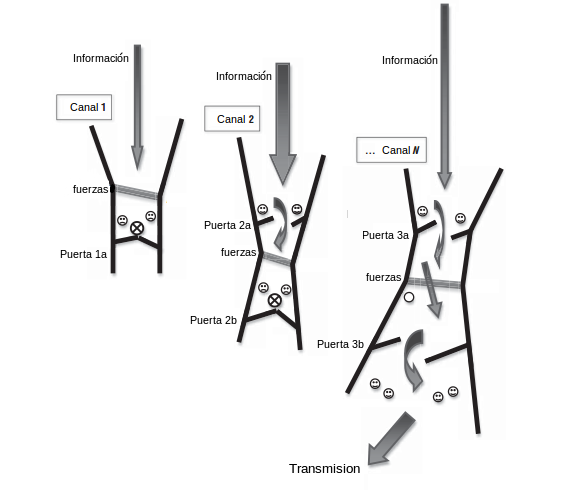
\includegraphics[width=0.6\textwidth]{imgs/gatekeeper.png}
  \caption{Representación del proceso de gatekeeper \cite{wahl2008handbook}}
  \label{fig:gatekeeper}
\end{figure}

La figura \ref{fig:gatekeeper} ilustra el proceso de \emph{gatekeeping} donde se muestran tres canales, muchos elementos de información y diversas fuerzas facilitan o dificultan el flujo de artículos a través de las diversas puertas, mediante la variación en la magnitud y la dirección del canal. Los elementos de información hacen su camino en los canales (que a veces se dividen en secciones) cada uno de los cuales se pueden introducir solamente pasando a través de una puerta. Las fuerzas negativas detienen el progreso de algunos elementos a través de los canales. 
El elemento final presentado como el resultado del proceso no sólo es el resultado de la selección, sino también de muchas otras fuerzas, ya que pasa a través de los diversos canales, secciones y puertas. Algunos procesos importantes están ocultos: Es el \emph{gatekeeper} quien controla si la información pasa a través del canal y el resultado final. Cabe señalar que los \emph{gatekeeper} toman muchas formas (ejemplo: personas, códigos profesionales de conducta, políticas de la empresa, los algoritmos informáticos, etc.) y todos toman decisiones, pero con distintos grados de autonomía. La autonomía varía desde idiosincrasias de una persona a conjuntos de reglas inquebrantables interpretados por algún algoritmo de un computador.

Las flechas varían en tamaño para indicar cómo los artículos cambian a medida que pasan a través de las diversas puertas o barreras. El elemento listo para ser transmitido es el resultado de muchas influencias y no siempre se parece al artículo original.

\section{Visiones referente al \emph{gatekeeping}}

Existen diversos análisis y críticas respecto al efecto y real impacto del proceso de \emph{gatekeeping} en la generación de una noticia.

White\cite{white} se refiere al proceso como ``muy subjetivo'' puesto que las diversas etapas dependen de juicios de valor basados en el conjunto propio de experiencias, actitudes y expectativas del \emph{gatekeeper}. En investigaciones posteriores White sostiene que la selectividad de los y las periodistas es la principal fuente de ``sesgo'' de las noticias gatillado, entre otras cosas, por la necesidad de reducir una multitud de acontecimientos ocurridos en el mundo real a un número modesto, en un tiempo reducido. 
%( 1950, p.386 )
%\footnote{White, D. M. (1950). The gate keeper: A case study in the selection of news. Journalism Quarterly, 27, 383–390}

 Breed en su investigación sobre el control social en las salas de redacción \cite{breed1955social} identifica a los y las editoras de los periódicos como los \emph{gatekeeper} de facto que operan a través de medios indirectos para asegurar que sólo las noticias en consonancia con la política de la organización sean las generadas. Breed agrega ``Las políticas de noticias podrían modificar o enterrar un evento y de esta manera denegar una información importante a la ciudadanía''.

%Although not a “gatekeeping” study as such, Warren Breed’s (1955) research on social control in the newsroom is a close contemporary of White’s and often mentioned together. In “Social control in the newsroom: A functional analysis,” Breed—also a former newspaper reporter— interviewed a sample of newsmen at medium-sized newspapers to determine how they discerned the appropriate way to handle their story selection. Breed, in a sense, identified newspaper pub-
%lishers as the de facto gatekeepers who operate through indirect means to ensure that only news consistent with organizational policy gets through. The relevant gatekeeping issue for Breed was that “policy news may be slanted or buried so that some important information is denied the citizenry” (p. 193).

Breed muestra cómo el \emph{gatekeeper} más importante puede no ser necesariamente quien esta relacionado más directamente con la selección ya que puede residir en otro lugar, dentro de los niveles más influyentes de la organización. Si la noticia es lo que el periodista dice que es, la subjetividad del \emph{gatekeeper} problematiza profundamente el proceso de información. Reese y Ballinger en \cite{13213947} argumentan que la razón radica en la expectativa de que actúe adecuadamente en nombre de la comunidad, \emph{el gatekeeper} ``ve a ella (a pesar de que nunca sea consciente de ello) que la comunidad oirá como un hecho único aquellos eventos que el periodista , como representante de su cultura, cree que es verdad''. Al igual que White, Breed señala que el proceso \emph{gatekeeping} podría funcionar cumpliendo las expectativas de la comunidad a través de los códigos periodísticos y otras orientaciones, fuera de la influencia indebida de las y los editores. 

%De acuerdo con estos puntos de vista, mientras los \emph{gatekeeper} se mantengan fieles representantes de la cultura, la sociedad no tiene por qué temer sus decisiones.

%Breed’s contribution was to show how the most important gatekeeper may not be the one who is most immediately involved in the selection, but may reside elsewhere within more influential levels of the organization. If news is what the journalist says it is, the subjectivity of the gatekeeper would seem to profoundly problematize the news process, and yet the field was slow to follow up on this key insight. Reese and Ballinger (2001) argue that the reason lay in the expectation that acting adequately on behalf of the community, the gatekeeper “sees to it (even though he may never be consciously aware of it) that the community shall hear as a fact only those events which the newsman, as the representative of his culture, believes to be true” (White, 1950, p. 390). Like White, Breed implied (as did subsequent interpretations by field synthesizers) that the gatekeeping process could work to the satisfaction of the community via journalistic codes and other guidance, were the undue influence of publishers to be curtailed. According to these views, then, as long as gatekeepers remained faithful cultural representatives, the society need not fear their decisions.

 En \cite{gans1979deciding} Gans identifica las fuentes de poder dentro de la organización periodística y los incentivos que tienen las y los periodistas para cumplir con las normas del grupo y seguir las consideraciones prácticas. Gans señala que la construcción de la noticia no está principalmente en el periodista o en el editor o editora, sino en el proceso por el cual todas las partes, las rutinas y las disposiciones de la organización se dedican a la creación de noticias. Reduciendo la responsabilidad directa respecto a la distorsión de individual de cada periodista.

Para Gans, el proceso de \emph{gatekeeping} es el proceso de solución de los problemas relacionados con el envasado del flujo diario de los acontecimientos, en un producto comercial para el público. Para solucionarlo, los periodistas utilizan ``consideraciones'' para ayudar en el proceso, que debe ser aplicables sin demasiada deliberación, éstas deben ayudar a evitar la incertidumbre excesiva, ser flexibles, fácilmente racionalizadas o explicables a los demás y eficientes, garantizando los mejores resultados con el menor esfuerzo. 

%La ecuación de prensa se basa en la eficiencia y el poder, que están estrechamente conectados.

Lewin \cite{lewin1951field} plantea que las y los individuos deben entenderse en el contexto de cuatro sistemas: un microsistema (contexto inmediato), mesosistema (nexo de contextos inmediatos), exosistema (instituciones externas) y macrosistema (cultura o sistema social). Estos cuatro niveles aplicados a la redacción de una noticia incluyen el nivel individual de cada periodista, el nivel de las rutinas o prácticas de periodismo, el nivel de organización, el nivel de los medios de comunicación y el nivel del sistema social. Lewin sostiene además que en todos los niveles existen diversas fuerzas que determinan cuales elementos se convierten en noticias y cuales no, limitando la autonomía de los \emph{gatekeeper} y dando forma a las noticias de manera consistente.

%A pesar de que no existen investigaciones sobre la naturaleza de estas fuerzas, aparentent varían dependiendo del nivel considerado. A nivel individual, por ejemplo, la investigación ha demostrado que no todos la toma de decisiones es impulsado por la reflexión consciente - que puede dar como resultado la misma facilidad de factores subconscientes, tales como una disponibilidad o heurística de la representatividad ( Nisbett y Ross, 1980 ). En el nivel de sistema social, por su parte , instituciones sociales crean " limitaciones y oportunidades a los que los medios de comunicación y los actores responden " ( Hallin y Mancini, 2004 , p. 296 ). Estas limitaciones y oportunidades que emergen basan en el desarrollo contemporáneo de las instituciones económicas , políticas y medios de comunicación. Contenido de las noticias es similar en un sistema social, porque los actores responden racionalmente a las mismas limitaciones y oportunidades. En la medida en que el entorno institucional puede producir más de un camino racional , podríamos esperar variaciones incluso entre actores racionales.

Lippman en \cite{lippmann1922public} señala taxativamente que ``el papel de la prensa es el de ser en cierto modo servidor y guardián de las instituciones'' y sugiere que las fuerzas planteadas por Lewin se relacionan con este ``rol'' que juegan los procesos de comunicación y los medios. Según Laswell en \cite{Lasswell2007Structure} este proceso realiza tres funciones: 
\begin{enumerate}
\item Vigilancia del entorno, revelando amenazas y oportunidades que afecten a la posición de valor de la comunidad y de las partes que la componen.
\item Correlación de los componentes de la sociedad en cuanto a dar una respuesta al entorno. 
\item Transmisión del legado social. 
\end{enumerate}
De una forma esquemática ha sido descrito este triple papel de esta otra manera: vigilancia, foro para la discusión y escuela.\cite{informacionsociedad} 

Smith \cite{tedsmith} explica precisamente una de estas tres funciones capitales, la de vigilancia del entono mediante la metáfora del \emph{perro guardián} \footnote{ ``...la tarea del \emph{perro guardián} suponía que cada periódico atacaría y defendería desde una posición determinada, y que del conflicto entre todos, surgiría la verdad (...) Hoy en día, por el contrario, la prensa abarca muy numerosos medios de noticias, tanto impresos como electrónicos. En esta categoría se incluye un escogido y selecto puñado de diarios y semanarios, los servicios cablegráficos, las noticias de redes radiofónicos y, sobretodo, las principales cadenas de televisión. En virtud de sus dimensiones y prominencia, son estos pocos medios de élite los que establecen el tono de los programas de cobertura para la mayor parte de la prensa''} señalando además que las y los periodistas, en cuanto críticos y críticas sociales y políticas, no desempeñan correctamente la labor encomendada a causa de carencias estructurales en estos cuatro aspectos: 

\begin{enumerate}
\item El ejercicio periodístico es básicamente una actividad de escaso rigor intelectual y con marcada tendencia a la simplificación. 
\item Las y los periodistas suelen carecer de conocimientos técnicos adecuados para la mayor parte de las cuestiones complejas de la vida actual.
\item El trabajo periodístico se ejecuta sin la reflexión y el sosiego que son deseables en una adecuada labor crítica. 
\item Es evidente la falta de una actitud juiciosa y equilibrada en la mayor parte de las y los periodistas, que renuncian a hacer un balance de los datos positivos y negativos para reducirse únicamente a una esquemática y simplificadora enumeración de defectos aparentes sin analizar las causas.
\end{enumerate}

Jean-François en \cite{revel1990conocimiento} crítica la tendencia a priori que inducen los distintos medios de prensa en las distintas noticias \footnote{``...la generación de noticias debe resultar de la información correctamente establecida, y no dirigir la elección de esa información a impulsos de un prejuicio selectivo, que metamorfosea la despiadada ferocidad para con unos en indulgencia y sin límites con otros (...) lo que predomina desgraciadamente en muchos periódicos de nuestro entorno sociocultural es el dirigismo apriorista en contra del poder, la predisposición condenatoria contra los actos emanados de las instituciones gubernamentales''}. Real, Agudiez, Príncipe en \cite{ESMPESMP0707110189A} afirman que actualmente existe un descontento y desilusión ciudadana con los medios de prensa pues éstos últimos no cumplieron con su parte del contrato social (la de velar por la transparencia y la difusión de ésta información). 

%El diario on–line Periodista Digital justifica las razones que han motivado el repudio de las audiencias: (...) los ciudadanos están rechazando a los viejos medios de comunicación, a los que considera comprados y mediatizados. Como consecuencia, esos medios tradicionales pierden cada día credibilidad y audiencia'. De hecho, las investigaciones sociológicas revelan que los consumidores de información están perdiendo la confianza en los periodistas y en los medios a pasos agigantados, porque los consideran al servicio no de la ciudadanía sino del poder y de sus intereses políticos y económicos".

Con una visión contraria Lorenzo Gomis en \cite{gomis1991teor} desarrolla la siguiente idea: los medios de comunicación y los periodistas no sienten interés por los problemas derivados de las posibles repercusiones de sus mensajes, pues no son ellos quienes los generan intencionalmente, sólo los comunican y los efectos de ambas acciones son incomparables \footnote{ Gomis lo explica de la siguiente manera: ``...La mayor influencia que se ejerce en los medios no es a través de los comentarios, sino de los mismos hechos. Y por lo tanto influye quien aporta el hecho, ya sea el interesado en el hecho que le favorece, o ya sea el interesado que perjudica a su adversario. Los medios son en definitiva la escena donde se luchan los productores de hechos para influir en la gente, mientras que los que controlan el medio sólo se interesan relativamente en esa pugna (...) Los más interesados en influir en los medios no son ni los que los poseen ni los que trabajan en ellos. Curiosa situación''}. Para este autor el accionar de los \emph{gatekeeper} no tiene motivaciones otras que no sean técnicas: ``Los seleccionadores o gatekeepers no ponderan la influencia potencial de los hechos en cuanto a sus efectos políticos o sociales, sino que consideran únicamente su condición técnica de noticia y, en caso de duda, es sumamente probable que la noticia quedará sin publicar''.

A finales de la década de los noventa surgió una alternativa a esta visión de los medios de prensa como una entidad que resguardaba de forma neutral los intereses de las y los ciudadanos, que implica a los mismos ciudadanos y ciudadanas, esto posibilitado -entre otras cosas- por la irrupción de Internet y las profundas transformaciones que supone en la información periodística y las vías de acceso a la información.

Las nuevas tecnologías brindan diferentes oportunidades para la incorporación de las inquietudes de las y los ciudadanos en los discursos dominantes de los medios mediante su participación directa en la producción informativa. Un nuevo escenario donde los pasivos y silenciosos ciudadanos se convierten en potenciales productores de información.

La adaptación de los medios de comunicación a este nuevo escenario, prevé una comunicación bidireccional entre medio y audiencia. En ese sentido, los medios de comunicación intentan consolidar mecanismos de participación en sus medios digitales. No obstante, tal y como señala Hermida en \cite{doi17512781003640703} en una investigación que examina las oportunidades que la audiencia tiene de participar en el proceso periodístico (participación, acceso, selección, edición y distribución) identifica que los medios de comunicación suelen ofrecer herramientas de participación similares entre sí y raras veces permiten que participe del \emph{gatekeeping} \footnote{``Nuestro estudio indica que la selección, o filtro, es el proceso de \emph{gatekeeping} más cerrado para los usuarios, y creemos que seguirá siéndolo'' \cite{doi17512781003640703}}. %pagina21

Shayne Bowman y Chris Willis presentan en su informe ``\emph{We Media}'' \cite{wethemedia} las valiosas ventajas de incorporar a las y los ciudadanos en la producción de información:
\begin{enumerate}
\item La posibilidad de pedir sugerencias y correcciones al público.
\item La posibilidad para las lectoras y lectores de que hagan comentarios.
\item La función de un filtro de noticias para noticias encontradas en la web a través de enlaces.
\item El control de exactitud en la información publicada.
\item El enriquecimiento de fuentes e ideas para periodistas gracias a las sugerencias e historias presentadas por las y los lectores.
\end{enumerate}
%(2003) 

Existe una gran cantidad de situaciones en las que las y los ciudadanos han colaborado con el envío de informaciones, imágenes y vídeos sobre un acontecimiento. Contribuyendo a comunicar un suceso desde su propia perspectiva. 
A ese fenómeno se le reconoce como periodismo ciudadano, periodismo de fuente abierta o periodismo en red, que son sinónimos de lo que Bowman y Willis denominan periodismo participativo en Internet. En \cite{wethemedia} lo definen como ``el acto de la ciudadanía que juegan un papel activo en el proceso de colectar, reportar, analizar y diseminar información'', que con frecuencia ocurre en un medio social y colaborativo. %(Bowman y Willis, 2003, p. 9).

En este proceso hay una comunidad de internautas que se reúnen para producir de forma colaborativa. En este caso, no existen límites geográficos, lo que cuenta es el conocimiento, el trabajo creativo y el deseo de colaborar. Esa comunidad de usuarios también se dedica a filtrar contenidos y recomendarlos a sus contactos en la Red. A este proceso Bruns en \cite{quteprints189} denomina \emph{gatewatching}. Que a diferencia del proceso de \emph{gatekeeping} no se busca seleccionar la información, sino de dar facilidades y atajos de lectura.

Los formatos más comunes para la participación en los medios de comunicación incluyen: Blogs de ciudadanos y ciudadanas, envío de fotografías y vídeos, envío de textos, entrevistas colectivas, comentarios, ranking de contenidos elaborados de acuerdo con los votos de usuarios, foros, blogs de periodistas, encuestas y comentarios en redes sociales como Facebook y Twitter \cite{doi17512781003640703}. %(Hermida, 2010).

Arriagada y Navia en \cite{intermedio2013} plantean que la irrupción de la tecnología no solo amplia las posibilidades de producción y acceso de la ciudadanía sino también modifica las relaciones de poder e influencia entre los medios, las audiencias y los grupos políticos, empoderando a las y los ciudadanos permitiendo el desarrollo de interacciones entre la clase política y la gente de forma independiente del quehacer de los medios \footnote{ Arriagada y Navia lo explican de la siguiente manera: ``Si históricamente los medios podían ser considerados como el cuarto poder, en tanto constituían una institución de la sociedad que podía vigilar el comportamiento de la clase gobernante, ahora los propios medios son a su vez vigilados por grupos que, a través de redes sociales online, participan activamente en los debates públicos, y que a menudo presentan niveles de desconfianza relativamente altos hacia las instituciones. En las redes sociales online, estos niveles de desconfianza pueden alcanzar también a los medios. Es más: en la medida que la gente percibe a los medios como parte de la institucionalidad o como representantes de las élites, los crecientes niveles de desconfianza en las instituciones también pueden alcanzarlos.'' }.
\newpage

\section{Twitter y su relación con el periodismo}

Además de red social, Twitter se ha convertido en un sistema de noticias compartidas en línea, que se basa en mensajes cortos, rápidos y frecuentes. Hermida \cite{hermida2010twittering}
%(2010) 
describe este sistema como un medio ambiente que muestra la información en un espacio ocupado por la o el usuario.
En este sistema, las y los usuarios reciben la información en la periferia de su conciencia, es decir, Twitter no requiere la misma atención cognitiva que un e-mail, por ejemplo. Se refiere a una especie de medio ambiente periodístico que ofrece diversos medios para recopilar, comunicar y compartir noticias e información. 

%En el trabajo periodístico, las redes sociales con plataforma de microblogging, como Twitter, favorecen tanto la difusión instantánea de la información corta (Hermida, 2010) como la movilidad (Silva, 2009). Conforme Silva (2009), Twitter forma parte de los moblogs, que también
%son utilizados como herramientas periodísticas. A la estructura de tecnologías móviles conectadas a Internet por wireless (móviles, smartphones, portátiles, tablets, etc.) que se suele usar durante la cobertura de un evento o suceso, Silva (2009, p. 260) la denomina como un ambiente móvil de producción, “que se vincula directamente al moblog periodístico ampliando las condiciones de movilidad del
%trabajo de campo”.

Debido al acceso a Twitter desde teléfonos móviles existe una nueva estructura de movilidad al periodismo, tanto en la producción como la difusión de la información, ya que la conectividad de los dispositivos móviles permite la instauración de la instantaneidad de la noticia. Siendo así, la movilidad reconfigura el trabajo de edición de blogs y la generación de contenidos periodísticos en las redes sociales. 
%(Silva, 2009).

Por su carácter instantáneo, Twitter sirve como plataforma para la realización de la cobertura periodística de eventos, en la cual se elabora un tipo de crónica de última hora o flash \footnote{El flash corresponde a una información de última hora, de elevada importancia y gran impacto informativo. Suele ser un texto conciso en que se priorizan los aspectos más relevantes del acontecimiento. De acuerdo con Salaverría el flash es solo un arranque de una cadena de informaciones, que resultará en un texto más completo que responda a las seis preguntas clásicas de toda noticia. El flash se ha ido convirtiendo en notas informativas cortas, limitadas a 140 caracteres (límite establecido por los servicios de mensajería instantánea y Twitter).\cite{salaverria2005redaccion}}, pero en orden cronológico inverso. 

Un guía oficial de Twitter para redacciones periodísticas fue lanzado en junio de 2011, en ella se señala: ``Twitter es una herramienta de todos los periodistas pueden utilizar para encontrar las fuentes más rápido, contar historias mejor y construir una mayor audiencia para su trabajo'' \cite{tweetsJournalist}.

					
	\chapter{Estado del Arte}\label{chap:estadodelarte}
	 \label{sec:estado_arte}

\section{Estudios relacionados}

\subsection{Clasificación de tweets y usuarios de Twitter}

Debido a la gran cantidad de usuarias y usuarios que forman hoy en día la red social de Twitter, la clasificación tanto de cuentas como de contenidos se ha convertido en una creciente materia de estudio para la comunidad científica. En el siguiente apartado se revisan los trabajos realizados referentes a ésta temática.

\subsubsection{Clasificación de usuarios}
   
     Pennacchiotti y Popescu en \cite{PennacchiottiP11} desarrollan una clasificación del perfil de las cuentas considerando principalmente cuatro aspectos diferentes:

    \begin{enumerate}
        \item \emph{Perfil del usuario}: Información básica de la cuenta como el nombre de usuario, la locación, una pequeña biografía además del número de seguidores y seguidoras, el número de personas a las que sigue  y el número de tweets. 
        
        \item \emph{Comportamiento para escribir tweets}:  Conjunto de métricas de las interacciones
        existente entre la red social y el usuario o usuaria: el número promedio de tweets por minuto, número de respuestas, entre otras. 
        
        \item \emph{Contenido lingüístico de los tweets}: Encapsula los temas principales de interés del usuario, así como su uso de léxico, este análisis mediante el uso de \emph{palabras prototípicas} \footnote{ El análisis se realiza mediante el uso de las cuales son expresiones típicas de las personas pertenecientes a una clase específica, así como frases relacionadas a intereses típicos de dicha clase} permite la clasificación de los usuarios y usuarias según su estilo de escritura tales como textos oficiales, blogs, conversaciones o traducciones.
       
        \item \emph{Información de Twitter}: Estas características exploran las relaciones sociales establecidas por
        la o el usuario con los demás que él o ella siguen, a quien le responde o que personas re-tweetea.          Pennacchiotti y Popescu indican que existe la idea intuitiva de que las personas pertenecientes a una clase son más propensos a seguir las cuentas de ciertas personas y a responder a ellas (por ejemplo, las jóvenes pueden tender a responder a la cuenta de Justin Bieber).
       
    \end{enumerate}

	        Respecto al análisis del \emph{Perfil del usuario} Pennacchiotti y Popescu tras analizar un corpus de
	        14 millones de cuentas, identifican que sólo el 48\% provee una biografía corta y 80\% una ubicación, de cuya información se intentaron determinar el género del usuario o usuaria y su etnicidad pero los resultados obtenidos fueron de muy baja calidad. 
	        
	        Mediante una muestra 15000 cuentas de forma aleatoria y un conjunto de editores y editoras a quienes se pidió identificar la enticidad y el género a partir de la imagen del avatar de Twitter. Se obtiene que menos del 50\% de las imágenes se correlaciona de manera clara con alguna etnia mientras que el 57\% se correspondía con algún género. Se identifica también que las imágenes podían ser engañosas: en el 20\% de los casos la imagen no corresponde al dueño o dueña de la cuenta sino de una celebridad o de otra persona.
	        
	         Con esta información estadística el estudio concluye que los campos del perfil del usuario no contienen suficiente información ni de buena calidad para ser utilizada para una clasificación.
	        %En trabajo anteriores Cheng en \cite{Cheng:2010:YYT:1871437.1871535} estableció que sólo el 26\% de los usuariosde Twitter reportan su ubicación como una ciudad específica, el resto provee locaciones generales (estados o paises) o lugares imaginarios. 
	        
	        
	        %En \cite{JavaEtAl:07} han ratificado percepciones intuitivas como: Cuando los usuarios postean rara vez pero tienen una gran cantidad de seguidores tienden a ser un buscador de información. Mientras que los usuarios que poseen URL's en sus propios tweets son proveedores de información. Rao en \cite{Rao:2010:CLU:1871985.1871993} sugiere que el estudio de estas componentes no es útil para la mayoria de las tareas de clasificación y que queda incluida en los rasgos lingüísticos.
	        
	        
	        Referente al \emph{Contenido lingüístico de los tweets} se realiza un análisis de los hashtag prototípicos, basados en la hipótesis de que si los usuarios o usuarias de una clase están interesados en los mismos temas, los temas más populares de esta clase se pueden encontrar mediante la recopilación de estadísticas sobre hashtags usados. A modo de síntesis se representa a un usuario mediante el conjunto de palabras de sus tweets y mediante éstas se intenta clasificar a dicho usuario.
	               
	         También se realiza un análisis de sentimientos a los distintos tweets, pues frente a un tema en particular dos clases pueden expresar distintos sentimientos. Por ejemplo: dos grupos políticos pueden expresar opiniones positivas o negativas de una figura pública dependiendo generalmentee si es del mismo sector político a ellos.  Para este proposito, se recoge un conjunto de palabras para las clases observadas en este estudio sobre las que el usuario particular tiene una opinión global que en su mayoría no es compartida por otra clase diferente.

    Las clases específicas estudiadas se refieren a: afiliación política, clasificación de si es o no seguidor de Starbucks y si los usuarios  y usuarias pertenecen o no a la etnia afroamericana. 
    
    %Los resultados obtenidos indican que para los dos primeras clases es posible conseguir un buen resultado con una considerable precisión, mientras que para el tercero es más compleja la tarea.

    Para determinar la afiliación política se concluye que las mejores características para su determinación son
    lingüísticas y de perfil. Siendo desconsiderable el aporte que entregan a esta determinación la información de Twitter y el comportamiento en "tweetear".

    `Para determinar si un usuario o usuaria pertenece a la clase \emph{seguidor o seguidora potencial de Starbucks} se identifica que  la \emph{información del perfil} y \emph{análisis lingüístico} son las  características más útiles para este objetivo.

    Se concluye además que la relación entre las y los seguidores y amigas y amigos es también una carácteristica relevante por sí sola para determinar la clase de seguidores o seguidoras, pues sugiere que los aficionados de Starbucks son los que siguen a los demás más que seguirse entre sí pues en su mayoría son los solicitantes de información (probablemente gente en busca de ofertas y cupones).

    Si bien el uso del léxico determina en este experimento con bastante precisión a la etnia afro-americana por sus variadas expresiones, cabe destacar que dichas expresiones ligúisticas han sido ampliamente adoptadas por otros grupos haciendo visible que esta característica posee una clara limitante en su aplicación. Los mejores resultados para determinar la etnia de un usuario es mediante la combinación del léxico y si siguen a celebridades a fines. Se encontró también que a tarea de clasificación puede ser ayudada por información del perfil.
  
 \subsubsection{Ranking de enlaces compartidos en Twitter}
  
  En \cite{Dong:2010:TEI:1772690.1772725} Dong utiliza como fuente de información fresca los contenidos y enlaces compartidos en Twitter para búsquedas web en tiempo real. Dong identifica que en vista de la investigación de  Hughes en \cite{hughes2009twitter} donde concluye que ante un evento inesperado, los tweets contienen más información relevante que en una situación normal (y tienen un enfoque más de \emph{broadcasting}), es posible considerar Twitter como una buena fuente de información en tiempo real en base a cuatro oportunidades:
  
  \begin{itemize}
	\item Los enlaces compartidos pueden corresponder a noticias o no (permitiendo recoger información sobre los enlaces que no son noticias y mejorar los resultados de la búsqueda).
	\item Los enlaces difundidos son publicados en base a las distintas prioridades personales de las y los usuarios, lo que aporta un interesante grado de diversidad.
	\item La red de Twitter permite realizar mediciones de autoridad a las y los creadores de tweets.
	\item Los tweets cuentan con metadatos relacionados que permiten clasificarlos e inferir en base a su relevancia.
  \end{itemize}
  
 Se consideran filtros en el procesamiento de enlaces referente al spam \emph{ Corresponden a enlaces propagados en Twitter referente a un producto o marca sin contenido relevante} basados en heurísticas a fines (como filtrar enlaces twitteadas por el mismo usuario más de dos veces o solo twitteadas por un mismo usuario).
 
 Referentes a los enlaces y los tweets que los contenían se consideran las siguientes carácterísticas:
  %Puesto que el sistema de Twitter se separa en dos componentes muy distintos, estos dos componentes que son: un sistema de publicación y otro de subscripción. El sistema de publicación permite detectar nuevas URL's mientras que el sistema de subscripción permite recoger información sobre la calidad de estas nuevas URL's.
  
\begin{itemize}
	\item \textbf{Características textuales}: Se considera que las palabras que acompañan a una URL en un tweet pueden entregar información relevante sobre ésta. Principalmente se realiza un conteo de estas palabras y la cantidad de repeticiones existentes para todos los tweets analizados, generándose un conjunto de pares de palabras y URL's relevantes (Similar al análisis del \emph{Contenido lingüistico de los tweets} considerado en el estudio analizado anteriormente \cite{PennacchiottiP11}).
	
	\item \textbf{Características de redes sociales}: Se aplica el concepto de autoridad a los usuarios de Twitter, vinculados mediante las relaciones de re-tweet entre ellos.
	
	\item \textbf{Otras características}: Se define un conjunto de diez características adicionales, muchas de las cuales consideran el ranking establecido en base a la autoridad de los usuarios. Estas se dividen en tres grupos:
		\begin{itemize}
		\item{Referentes al promedio del conjunto de usuarios que publicaron la URL}: número promedio de \emph{followers} de las y los usuarios, número promedio de tweets de las y los usuarios, numero promedio de las y los usuarios que retweetean cantidad de tweets que contienen la URL, promedio de usuarias y usuarios que responden los tweets que contienen la URL, promedio del número de usuarias y usuarios a las que siguen, promedio del ranking de autodidad (definido anteriormente).
		\item{Referentes al usuario que inicialmente twitteó la URL}: Se asume autoridad para el primer emisor de la URL en base a algunos criterios como número de followers, número de tweets, número de usuarios que realizaron retweet, número de respuestas, número de personas a las que sigue.
		\item{Referentes al usuario que posee mayor ranking de autoridad} Las características observadas son número de followers, número de tweets, número de usuarios que realizaron retweet, número de respuestas, número de personas a las que sigue y el ranking de autoridad.
		\end{itemize}
\end{itemize}
	
	El ranking se basa en una máquina de aprendizaje de ranking (MLR) que considera las características anteriores con distintas ponderaciones de importancia calificándolas con un factor en una escala de [0,100] (de forma descendente, las más importantes son: La característica de repetición de la URL en los distintos tweeets y su relación con las palabras relacionadas, número de seguidoras y seguidores del usuario con mayor grado de autoridad, número de usuarias y usuarios que re-tweetan la URL al usuario con mayor grado de autoridad, número promedio de usuarios y usuarias que re-tweetean los tweets que contienen la URL y número promedio de usuarios y usuarias que siguen a quienes han twitteado la URL). Los resultados se clasificaron en base a una tupla (query,URL,$t_query$) con grados de relevancia y se constrataron con la opinión de cinco expertos en cinco grados de clasificación: perfecto, excelente, bueno, justo y malo. Se agrega además un sistema de etiquetas de tiempo debido al interés especial de esta dimensión del problema, donde los tweets fueron clasificados en dos grandes categorías: sin sensibilidad de tiempo y con senbilidad de tiempo con las subcategorías: \emph{reciente}, \emph{de alguna manera reciente}, \emph{de alguna manera fuera de fecha} y \emph{totalmente fuera de fecha}.
	
	Si los documentos cuentan son de la categoría: \emph{sin sensibilidad de tiempo}, \emph{reciente} o \emph{de alguna manera reciente} al momento de su clasificación preservan su clasificación, en cambio, cuando son \emph{sensibles al tiempo} se utiliza un sistema de descenso de categoría:
	
	\begin{itemize}
		\item \emph{Descenso de un grado}: Si el resultado es \emph{de alguna manera fuera de fecha} se realiza un descuento de un grado (por ejemplo de excelente a bueno).
		\item \emph{Descenso de dos grados}: Si el resultado es \emph{totalmente fuera de fecha} se realiza un descuento de dos grados (por ejemplo de excelente a malo).
	\end{itemize}
	
	Los resultados obtenidos fueron contrastados con expertos bajo el criterio de que sólo evaluaran una query como "con contenidos relevantes de última hora" si el sistema arrojaba al menos un documento creado en las últimas 24 horas con contenido relevante. Se obtuvo que el 91,7\% de las consultas fueron clasificados de esta manera y que una gran cantidad de URL's poseen la calidad de enlaces frescos, lo que hace concluir que casi no existen documentos obsoletos en las URL's de Twitter. 
	
	Se identifica también que el porcentaje de edades de los enlaces clasificados como \emph{perfectas} o \emph{excelentes} es más alta comparativamente que los enlaces \emph{regulares}, mientras que las clasificadas como \emph{justo} y \emph{mala} son más bajas que las URLs \emph{regulares}, demostrando de esta manera que las características de Twitter pueden mejorar el rendimiento de un sistema de \emph{ranking} sensible al tiempo.  
	
	Finalmente se concluye que los enlaces propagados en Twitter son útiles para mejorar potencialmente la clasificación de consultas de búsqueda sensibles al tiempo.
	
\subsubsection{Mecanismo de Ranking en Twitter como foro}

	 En \cite{DasSarma:2010:RMT:1718487.1718491} se presenta un análisis de un sistema de ranking que podría ser perfectamente aplicado a Twitter por sus características, sugiriendo una arquitectura genérica de un sistema de clasificación para diversos items (tweets, post u otro) con la intención de conseguir la mejor clasificación posible con el menor esfuerzo implicado.

Las características deseadas para el sistema de ranking propuesto son:

	\begin{itemize}
		\item \emph{Precisión del Ranking}: El ranking debe ser preciso aún cuando no sea posible re-evaluar nuevamente todos los items implicados.
		
		\item \emph{Revisión del ancho de banda}: El ranking debe converger al orden correcto, dentro del nivel de precisión deseado rápidamente con una pequeña cantidad de retroalimentación por artículo.
		
		\item \emph{Baja Latencia}: Los usuarios y usuarias no deben esperar mucho tiempo para recibir un estimado de sus puntuaciones o clasificaciones actualizadas.
		
		\item \emph{Equidad}: Los items deben ser tratados igualmente con respecto a la clasificación y la revisión.
	\end{itemize}

	Debido a que la distribución de probabilidad con la cual son evaluados los diversos elementos, su evaluación depende principalmente del orden en que son presentados, se intenta contrarrestar este efecto mediante el diseño de formas explicitas de evaluación en este trabajo. Bajo esta misma perspectiva, se elige
	el método de evaluación comparativo entre dos elementos a modo de torneo, el cual funciona de la siguiente manera: cuando el usuario o usuaria envía un nuevo elemento (tweet, comentario o post) se le muestra un par de otros items (seleccionados dependiendo la distribución de torneo sorteada al azar) entre los cuales selecciona el mejor, dichas clasificaciones son recogidas y evaluadas (estas evaluaciones cuentan con una mejor estimación de rango entre más evaluaciones poseen dichos elementos).
	
	Se concluye que el sistema de \emph{ranking} planteado posee mejor rendimiento -evaluado en base a las carácterísticas deseadas- que un sistema de calificación individual (como el sistema de clasificación por estrellas de plataformas como Netflix).
	
\subsubsection{Twitter para la recomedación de noticias}

	Muchos de los sistemas actuales de recomendación, se basan en las preferencias personales de los usuarios, en \cite{Phelan:2009:UTR:1639714.1639794} utiliza Twitter y fuentes RSS para este cometido.
	
	El sistema se compone de tres grandes componentes:
	\begin{itemize}
		\item \textit{Componente Web}: Encargada de reunir la información disponible del usuario en RSS y en Twitter para recoger las preferencias de la usuaria o usuario.
		\item \textit{Index Lucene\footnote{Lucene es una biblioteca de búsqueda de texto completo extremadamente rica y poderosa escrita en Java}}: Responsable de la indexación y la minería de la información obtenida.
		\item \textit{Recomendación}: Encargado de generar una lista clasificada de historias RSS basado en la co-ocurrencia de términos populares dentro de los post y gustos expresados en Twitter.
	\end{itemize}
	
	La indexación se genera principalmente al transformar las palabras contenidas en los últimos tweets del usuario en una matriz de co-ocurrencia $M$ ($M_{ij}$ representa la cantidad de ocurrencias que posee la palabra $j$ en
	el tweet $i$), las co-ocurrencias mayores se relacionan con el conjuntos de artículos que las contienen, tras sumar esta cantidad se le asigna un puntaje basado en la sumatoria de co-ocurrencias evaluadas. De esta forma, se crea un ranking de temas y artículos a sugerir (ordenados entre estos mismos según su grado de relevancia). 
	
	Por otra parte el usuario puede elegir tres estrategias distintas de recomendación: 
	
	\begin{itemize}
		\item \textit{Ranking Público}: Basado en el análisis de los tweets públicos del timeline del usuario.
		\item \textit{Ranking de las y los amigos}: Basado en el análisis de los tweets públicos de los timelines de los amigos y amigas del usuario.
		\item \textit{Ranking de Contenido}: No utiliza Twitter, sólo considera las 100 mayores ocurrencias de palabras del análisis de las RSS.
	\end{itemize}
   
   Se evalúa la aceptación de las recomendaciones realizadas por este sistema mediante el criterio de un pequeño grupo de 10 participantes, en un período de 5 días y se cuantifica la cantidad de clicks recibidos por noticia recomendada por el sistema. Cada participante configuró el sistema con su información correspondiente.

	Al analizar los resultados se obtiene una clara diferencia en el comportamiento de las y los usuarios cuando se comparan las estrategias basadas en Twitter a la basada en el contenido predeterminado. Se observa, por ejemplo, que para la primera prueba se recibe una media 8,3 y 10,4 \emph{clicks} por cada usuario en comparación con sólo el 5,8 \emph{clicks} por usuario en la estrategia basada en el contenido; expresando un relativo aumento de entre el 30\% y el 45\% para las estrategia basada en Twitter.

	Se observa también que el \emph{ranking} de mayor uso de las recomendaciones basadas es el \emph{ranking de las y los amigos} en comparación a las recomendaciones del \emph{ranking público}, resultado que se contradice con un cuestionario posterior realizado, donde un 67\% de las y los usuarios indican su preferencia por \emph{ranking público} mientras que sólo el 22\% señala su preferencia por el \emph{ranking de las y los amigos}. Ninguno de los participantes se muestra partidario de la estrategia de \emph{ranking de contenido} y un 11\% no saben cual estrategia prefieren.

\subsubsection{Clasificación de tweets orientada al usuario: Un enfoque de filtrado para microblogs}

%En  se plantea la relevancia de un filtrado de contenido en Twitter, ya que debido a su enorme volumen de información carece de valor sin no es presentada de manera adecuada. 

Ibrahim y Bruce en \cite{conf/cikm/UysalC11} plantean que la acción de re-tweetear para clasificar a los usuarios posee un gran valor: re-tweetar incluye leer el tweet, decidir que vale la pena compartir y luego actuar sobre ella, por lo cual es posible considerar el re-tweet como una señal explícita de que la usuaria o usuario considera el tweet como información relevante. Basado en esta apreciación, se busca dar respuesta a la interrogante  ¿Es posible clasificar a los usuarios basado en si re-tweetean un tweet específico?

El objetivo de este trabajo es clasificar la cuenta de un usuario para mostrar los tweets entrantes en un orden descendente en función de su probabilidad de ser retweeteado por el mismo. Una clasificación efectiva ayudará al usuario a encontrar los tweets potencialmente más interesantes. Como experimento preliminar, se utiliza un árbol de decisión (J48) (implementado en WEKA) para determinar la precisión con la que se puede clasificar los tweets como re-tweetable o no para un usuario específico. Se entrena el clasificador se utilizan cuatro grupos de rasgos:

\begin{itemize}
	\item \textit{Basado en el autor}: Se refiere a características deducidas a partir del perfil del usuario, relacionadas a qué tan activo es el usuario o usuaria y la autoridad que posee.: ¿Es el usuario un autor de élite \footnote{\emph{élite} local si su cantidad de seguidores esta en el rango de 10K-50K followers, \emph{élite global} si su cantidad de followers es mayor a 50K y \emph{usuario ordinario} si el usuario tiene de 10 a 1000 seguidores o personas a las que sigue, escribe entre 1 a 200 tweets por semana y ha twitteado más de 10 veces.} ?, cantidad de followers, cantidad de personas a las que sigue, cantidad de tweets,  edad del perfil \footnote{cantidad de días desde la creación de la cuenta}, tasa de tweets, cantidad de favoritos, ¿tiene descripción?, ¿su idioma es el inglés?. 
	
	\item \textit{Basado en los tweets}: Se refiere a características sintácticas del tweet, algunas de éstas dan implicaciones sobre que tan bien está escrito el tweet: la categoría, la audiencia y la popularidad del tweet.: La puntuación TF-IDF\footnote{TF-IDF es una estadística numérica que se pretende reflejar la importancia de una palabra es un documento, colección o corpus}), ¿contiene hashtag? ¿contiene urls?¿Menciona a otros usuarios? ¿utiliza comillas para citar? ¿escribe el mismo carácter tres veces seguidas (por ejemplo: hoolaaa)?¿utiliza emoticonos?, la cantidad de re-tweet del tweet y el largo promedio de los tweets.
	
	\item \textit{Basado en el contenido}: Se refiere a las características relativas al contenido del tweet: novedad del tweet (distancia coseno de términos de los otros tweets que aparecen en el timeline en la última semana) y lo inesperado del tweet (distancia mínima de la distancia coseno de términos con los demás tweets del autor).
	
	\item \textit{Basado en el usuario}: Características relacionadas a la cuenta del usuario: Del tweet re-tweteado ¿sigue el usuario al autor? ¿utiliza el hashtag del tópico relacionado en otros tweets? ¿se comparten enlaces con el tweet? ¿se menciona al usuario en el tweet en cuestión?
\end{itemize}

Para el conjunto de entrenamiento se realizan dos clases: los tweets re-tweteados y los que no son re-tweeteados. Los resultados obtenidos señalan que ningún grupo de características arrojó resultados satisfactorios por si solos, entre las cuales la mejor característica de todas es la tasa de tweets (cantidad de tweets por semana). De las características basadas en los tweets las más valiosas fueron: si el tweet fue re-tweteado y la puntuación tf-idf. De las características basadas en  el usuario se considera útiles las características: "¿es el autor del tweet una persona a la que el usuario sigue?","¿se compartieron enlaces con el usuario?", "¿se utilizó el hashtag del tópico relacionado en otros tweets?" y "¿se menciona al usuario en el tweet en cuestión?".

\subsubsection{TURank: Clasificación del usuarios de Twitter basado en el análisis de un grafo usuario-tweet}

 En \cite{Yamaguchi:2010:TTU:1991336.1991364} se aborda el problema de identificar los usuarios con autoridad en una red de microblogging como es Twitter. Se entiende por un usuario con autoridad aquellos usuarios que frecuentemente suben información a la red, que es considerada relevante y es propagada de forma rápida y amplia.
 
 Debido a la gran cantidad de información que se encuentra en esta red social es preciso identificar los usuarios con autoridad que dinamizan y aportan con información relevante, su identificación podría tener múltiples impactos en el manejo y categorización de la información. Muchos trabajos enfocan su análisis en la estructura de vínculos de seguidores que mantienen los usuarios, sin embargo, la mayoría de las y los usuarios siguen de vuelta al usuario que comenzó a seguirlos por un acto de cortesía formal, por lo cual se considera poco relevante. En este trabajo se plantea un algoritmo que considera la puntuación de autoridad de los usuarios de Twitter considerando un grafo de relaciones sociales además del análisis del flujo de tweets entre los usuarios (mediante el re-tweet).

En Twitter, un usuario sigue a otro, si es probable que el usuario transmita información útil incluso sin garantías. En muchos casos, los seguidores no dejan de seguirlo incluso si resulta que no transmite  más información útil. Esto ocurre porque los usuarios no recuerdan a todos las usuarias y los usuarios a los que están siguiendo y debido al gran número de cuentas a las que el usuario sigue (de 100 a más de 1000 en muchos casos). Incluso si un usuario tiene una gran cantidad de seguidores no implica que estos sean frecuentemente re-tweetados.

En cuanto a la propagación de la información, cabe señalar que los re-tweets tienen distintas características dependiendo del objetivo que esta acción tenga, si es un re-tweet conversacional tiene sólo re-tweets de los implicados en dicha conversación, muy por el contrario si es un re-tweet de difusión, este tiene un  gran número de re-tweet y se propagan ampliamente. Por lo anterior, no es suficiente sólo contabilizar la cantidad de re-tweets para medir la autoridad de una usuaria o usuario, ya que los re-tweets conversacionales son menos relevantes para la puntuación de autoridad en cuestión. 

%Se consideran además los re-tweet realizados por usuarios con autoridad, pues es probable que estos retweets son más útiles que retweets de usuarios que no son autoridad.

Se utiliza un tipo de grafo direccional llamado \emph{esquema de transferencia de autoridad} donde se representan el dominio del discurso y los flujos respectivos de autoridad donde cada nodo representa todo el conjunto de elementos de destinos y las aristas todo el conjunto de relaciones o trasferencias que puede ocurrir entre ellos. Este gráfico es evaluado mediante \emph{ObjectRank} \footnote{ObjectRank es una extensión de PageRank\cite{ilprints422} para medir la importancia de los objetos en una base de datos teniendo en cuenta el tipo de aristas del grafo así como el tipo de nodo}.

La evaluación de los distintos usuarios y usuarias se basa en tres observaciones:

\begin{itemize}
	\item Una usuaria o usuario seguido por muchas autoridades probablemente es también una autoridad.
	\item Un tweet re-tweeteado por alguna autoridad probablemente sea un tweet útil.
	\item Una usuaria o usuario que posee muchos tweets útiles es probablemente una autoridad.
\end{itemize} 

Basado en estas observaciones fue construido un grafo donde los nodos representan usuarios y tweets mientras que las aristas representan las relaciones entre usuarios y tweets. Este grafo \emph{usuario-tweet} permite comprender cómo se propaga la información entre los usuarios mediante el re-tweet. Posteriormente se realiza un análisis de enlaces y se calcula la autoridad de los usuarios utilizando \emph{ObjectRank}. Las pruebas realizadas fueron contrastadas por un conjunto de expertos, y se obtuvo como conclusión que el número de followers y la cantidad de re-tweet no son suficientes para determinar si un usuario posee o no autoridad. El cuantificador de re-tweet tiende a extraer a los usuarios que utilizan el re-tweet para las conversaciones con el fin de especificar al usuario al cual se dirigen, en estos casos los tweets no trasmiten información útil.

Se demuestra que a pesar de su estructura simple, el grafo planteado describe las relaciones usuario-tweet lo suficientemente bien, representando adecuadamente las cadenas de re-tweet y múltiples re-tweets realizados por el mismo usuario o usuaria. Por otra parte, el ranking planteado es un eficaz sistema de puntuación para evaluar la autoridad de los usuarios de Twitter ya que evalúa a las usuarias y usuarios que no son seguidos por muchos usuarias y usuarios, pero sus tweets son re-tweeteados muchas veces, con una mayor posición mientras que a las usuarias y usuarios cuyos tweets no se re-tweetean, incluso si tienen un gran número de seguidores, se les asigna una peor la posición en el \emph{ranking}. Por último, a aquellas usuarias y usuarios en los cuales la mayoría de sus tweets son conversaciones, son evaluados como completamente inútiles por el algoritmo. 


\subsection{Geolocalización de usuarios} \label{sebsec:geoestadoarte}

 Cheng en \cite{Cheng:2010:YYT:1871437.1871535} identifica que la función de geolocalización en Twitter no es una función muy utilizada por las y los usuarios tras el análisis de una muestra aleatoria de más de un millón de usuarios, en la cual sólo el 21 \% señala el campo \emph{ubicación} del usuario como un nombre granular de una ciudad (por ejemplo: Los Angeles, CA) y sólo 5 \% señala una ubicación tan granular como coordenadas de latitud / longitud (por ejemplo: "29.3712 , 95.2104" ), el resto son demasiado generales (por ejemplo: California o España), no indican nada o uno sin sentido (por ejemplo: país de las maravillas). Como medio complementario para esta función, Twitter cuenta con la función de etiquetas geográficas ahora asociada a cada tweet. Pero a similitud del caso anterior, se observa que menos del 0,42 \% de todos los tweets realmente utilizan esta funcionalidad.

McGee en \cite{McGee:2011:GST:2063576.2063959} investiga la relación entre la fuerza del vínculo social entre un par de usuarios y la distancia entre dicho par con un conjunto de 6 millones de usuarios geolocalizados. En este estudio se observa que en una distribución bimodal en Twitter, con un pico de 10 kilómetros de las personas que viven cerca, y otro pico alrededor de 6.430 kilómetros, lo que valida el uso de Twitter tanto como una red social (con amigos geográficamente cercanos) y una plataforma de medios sociales (con conexiones muy distantes). También se observa que las y los usuarios con mayor fuerza en su vínculo (la amistad recíproca) tienen más probabilidades de vivir cerca entre sí que las usuarias y usuarios con vínculos débiles.

Cheng propone un marco de trabajo para la localización de usuario, que cumpla con las siguientes características:
\begin{itemize}
 \item Generalizable a través de las redes sociales.
 \item Robusto ante el ruido propio de los tweets.
 \item Confiable y preciso.
 \item Que trabaje únicamente con datos de dominio público por parte del usuario sin necesidad de análisis de otros datos de privacidad sensible (IP, usuario/clave, etc.).
\end{itemize}

El marco de trabajo propuesto se basa en la noción que los tweets incluyen algunos contenidos de ubicación específica, como nombres específicos de lugares o palabras que se refieren a ciertos lugares además de otras denominaciones locales para los mismos (por ejemplo: "Valpo" para referirse a Valparaíso), y que con dicha información es posible cubrir la falta de una geolocalización para los usuarios. La estimación de la localización basándose en el contenido es una tarea difícil puesto que los tweets son inherentemente ruidosos, a menudo con expresiones coloquiales y vocabulario no estándar. No es obvio en lo absoluto que existan señales claras de ubicación incrustados en los tweets de algún usuario. Una usuaria o usuario puede tener intereses que abarcan múltiples ubicaciones y tener más de una ubicación física.

Este estudio acotado a los usuarios dentro del territorio continental de Estados Unidos. El primer filtro realizado se realiza con las ubicaciones del tipo: 'NombreCiudad', 'NombreCiudad, NombreEstado', 'NombreCiudad, AbreviaciónEstado' (considerando todas las ciudades válidas que figuran en el censo 2000 en EEUU). Para los casos en que existían dos ciudades con el mismo nombre, para determinar la ambigüedad, sólo se tienen en cuenta si poseen información adicional respecto al estado en el cual se ubican. Tras aplicar este filtro se encontró que sólo el 12\% de los usuarios de la muestra fueron identificados. La segunda metodología implementada busca determinar la ubicación en base al contenido de los tweets de una usuaria o usuario, caracterizándolo por la distribución probabilista de sus palabras. Los resultados obtenidos con este enfoque es que sólo el 10.12\% de los usuarios pueden ser localizados a 160 kms. de sus ubicaciones reales (con una distancia de error promedio de 2.853 kms.). Se concluye que este enfoque no aporta resultados de calidad debido a:

\begin{itemize}
    \item La mayoría de las palabras se distribuyen de manera compatible con la población a través de las diferentes ciudades, lo que significa que la mayoría de las palabras ofrecen muy poco potencial para distinguir la ubicación de un usuario.
    \item La mayoría de las ciudades, sobre todo con un población pequeña, tiene un conjunto escaso de palabras en sus tweets, lo que significa que la distribución de palabras por ciudades para estas ciudades, están subespecificada, lo que conduce a grandes errores de estimación.
\end{itemize}

La tercera metodología determina la posición geográfica mediante la identificación de palabras locales en los tweets de los usuarios, basada en la noción que existen palabras que son más utilizadas en un ámbito geográfico que otros. Dichas palabras características son conocidas como palabras  \"locales" y atribuidas a un territorio específico, si éstas son aisladas son capaces de distinguir a los usuarios situados en una ciudad y no en otra. 

El trabajo concluye que existe una gran posibilidad de clasificación considerando y aislando estas palabras debido a su potencial y establece un método para su tratamiento. 

Las metodologías anteriores solo utilizaban como recurso de información los tweets, también en este trabajo se intenta obtener información adicional para localizar una persona basado en las relaciones entre usuarios en la red social. El vecindario de un usuario se determina mediante un vecindario difuso. Considerando a dos usuarios con una relación fuerte, cuando ambos usuarios se siguen mutuamente. Finalmente con la combinación de las metodologías se logra una metodología de posicionamiento geográfico basado en la información de Twitter, el análisis lingüístico de sus tweets y el análisis de sus relaciones sociales con una precisión de 54.26\% y una distancia de error promedio de 760 kilómetros.

Basado en la tercera metodología planteada por  \cite{Cheng:2010:YYT:1871437.1871535}  Graells y Poblete en \cite{GraellsGarridoP13} desarrollan una técnica de posicionamiento geográfico para usuarios en territorio Chileno con intenciones de corroborar si la población virtual en Twitter es representativa respecto a su ubicación a la población física. Se utiliza un modelo de espacio vectorial, que dado el contenido de un tweet, permite (a través de un clasificador construido sobre modelos de lenguaje) establecer su ubicación geográfica. 

Mediante un clasificador TD-IF y asumiendo que existen hashtags locales que se refieren a una ubicación concreta, es posible deducir la ubicación de un tweet con las palabras que co-ocurren junto a estos hashtags. Finalmente se concluye que los participantes en Twitter son representativos de la población física, es decir también responden al centralismo del país.

 %El enfoque basado en el contenido se basa en dos refinamientos clave: ( i ) un componente de clasificación para la identificación automática de palabras en tweets con un fuerte geo - ámbito local, y ( ii ) un modelo de suavizado barrio basado en celosía para refinar estimación de la localización de un usuario. Hemos visto cómo la ubicación estimador puede colocar el 51\% de los usuarios de Twitter a 100 millas de su ubicación real .

%Utilizando el conjunto de ensayo descrito en la Sección 3, seleccionamos al azar 500 usuarios, y rastreamos sus relaciones sociales. 354 usuarios de los 500 usuarios satisfacen nuestra condición con al menos 10 a 20 amigos conectados fuertes, donde definimos un fuerte amigo conectada de un usuario como alguien que es a la vez siguiendo y siguió por el usuario. Para cada uno de los 354 usuarios, nos arrastramos fuertes amigos conectados de los usuarios, y sus últimos 500 tweets. En total, tenemos 3.137.233 tweets de 6.502 usuarios que son fuertes amigos conectados del 354users.Recall que para cada uno de los 354 usuarios, tenemos la ubicación del usuario en forma de coordenadas de latitud / longitud. Con este conjunto de 354 usuarios y sus últimos tweets de 1000, aplicamos el mejor enfoque impulsado por el contenido identificado en los experimentos anteriores: Palabras locales Filtrado + Barrio Smoothing. Nos parece que este planteamiento impulsado por el contenido (sin refinamiento social), se traduce en una precisión de 54.26\% y una distancia de error promedio de 472,26 millas.




\section{Herramientas y plataformas relacionadas}

\subsection{Geofeedia}

Geofeedia \cite{geofeedia} es un servicio pionero en el control de origen de los medios de comunicación social mediante geolocalización, permite el monitoreo y  realizar análisis a datos provenientes de las redes sociales, complementando la tradicional búsqueda de \emph{keywords} que tipicamente pierden información de la actividad social relacionada, ayudando a reducir el desorden de los medios sociales en tiempo real, mejorando los descubrimientos escondidos de la información geolocalizada. Geofeedia realiza búsquedas en las redes sociales: Twitter, Instagram, YouTube, Picasa, y Flickr.

Posee una interfaz intuitiva y fácil de usar además de un conjunto de herramientas para facilitar las búsquedas. Geofeedia permite obtener stream de datos de redes sociales provenientes de una zona geográfica en específico, mediante la mención textual del lugar o la delimitación de una región en un mapa interactivo.

Los diversos feeds se pueden categorizar y "olvidar" usuarios (no recibir feed de dicho usuario). Los resultados de la búsqueda se pueden filtrar por fecha, por palabras claves, por tipo de medio social y por autor, entre muchos otros. La plataforma además permite variadas herramientas de análisis como identificar la tendencia de palabras claves, la actividad basada en el tiempo, frases influyentes, las fuentes de los medios sociales.

Los datos se pueden exportar a través de la API con todas las funciones de Geofeedia en formatos CSV ATOM, GeoRSS, JSON, KML.

\begin{figure}[H]
	\centering
	\begin{minipage}[t]{.45\textwidth}
		\begin{center}
			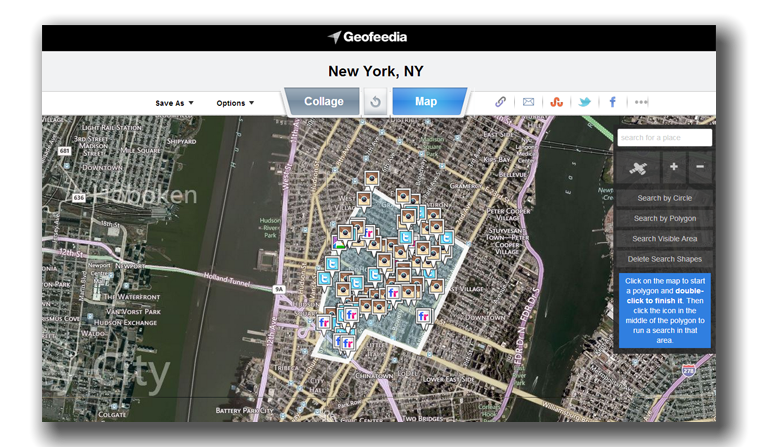
\epsfig{file=imgs/geofeedia1.png, width=2.5in} 
			  \caption{Imagen del mapa interactivo de geofeedia donde en una zona delimitada por el usuario se reciben todos los feeds de los medios sociales.}
			  \label{fig:geofeedia1}
		\end{center}
	\end{minipage}
	\hfill
	\begin{minipage}[t]{.45\textwidth}
		\begin{center}
			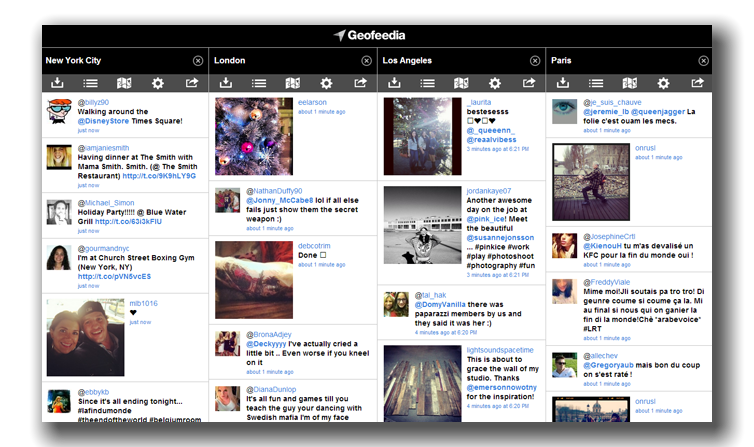
\epsfig{file=imgs/geofeedia2.png, width=2.5in} 
			\caption{Imagen del panel de noticias de geofeedia, donde cada columna recoge los feeds para ubicaciones geográficas distintas.}
			\label{fig:geofeedia2}
		\end{center}
	\end{minipage}
	\hfill
\end{figure}

\subsection{Paper.li}\label{subsec:paperli}

Paper.li \cite{paperli} es una creación de la startup suiza Small-Rivers con sede en Lausanne. Es una herramienta que permite generar una especie de periódico personalizado en base a las publicaciones en redes sociales de los contactos (en dichas redes) del usuario. Actualmente Paper.li permite el acceso a fuentes como Twitter, Facebook, Google, YouTube y los canales RSS para la recolección de información.

Permite fáciles combinaciones de las distintas fuentes de contenido, la priorización temática, la aplicación de filtros de contenidos, configurar las fuentes de información y personalizar el aspecto del periódico personal.

El funcionamiento de Paper.li se basa en el hecho de que muchos usuarios de Twitter confían más en el criterio de selección de sus redes sociales para identificar enlaces a noticias importantes que en las compilaciones que realizan los diarios tradicionales. Paper.li recoge los enlaces a noticias, fotos y vídeos de una cuenta en Twitter y otras redes sociales;  realiza una selección de estos vínculos (a partir de un análisis realizado con “herramientas de análisis semántico de texto”), crea una página diaria editada con aspecto a una página de los periódicos tradicionales que vemos en Internet, donde los enlaces y el contenido aparecen divididos en secciones contextuales.

Los creadores de Paper.li (mediante el blog oficial del medio) han declarado que la motivación inicial para crear este medio “no es por la sobrecarga de información es por la ausencia de un filtro“. Es importante señalar que Paper.li no cumple exactamente con la tarea de entregar las noticias de forma urgente debido a su intervalo de actualización diario, Paper.li más bien, reporta el eco de ellas en las redes sociales, la reproducción de contenidos más frecuentes, los tópicos más consultados o lo más recomendados.

\begin{figure}[H]
	\centering
	\begin{minipage}[t]{.45\textwidth}
		\begin{center}
			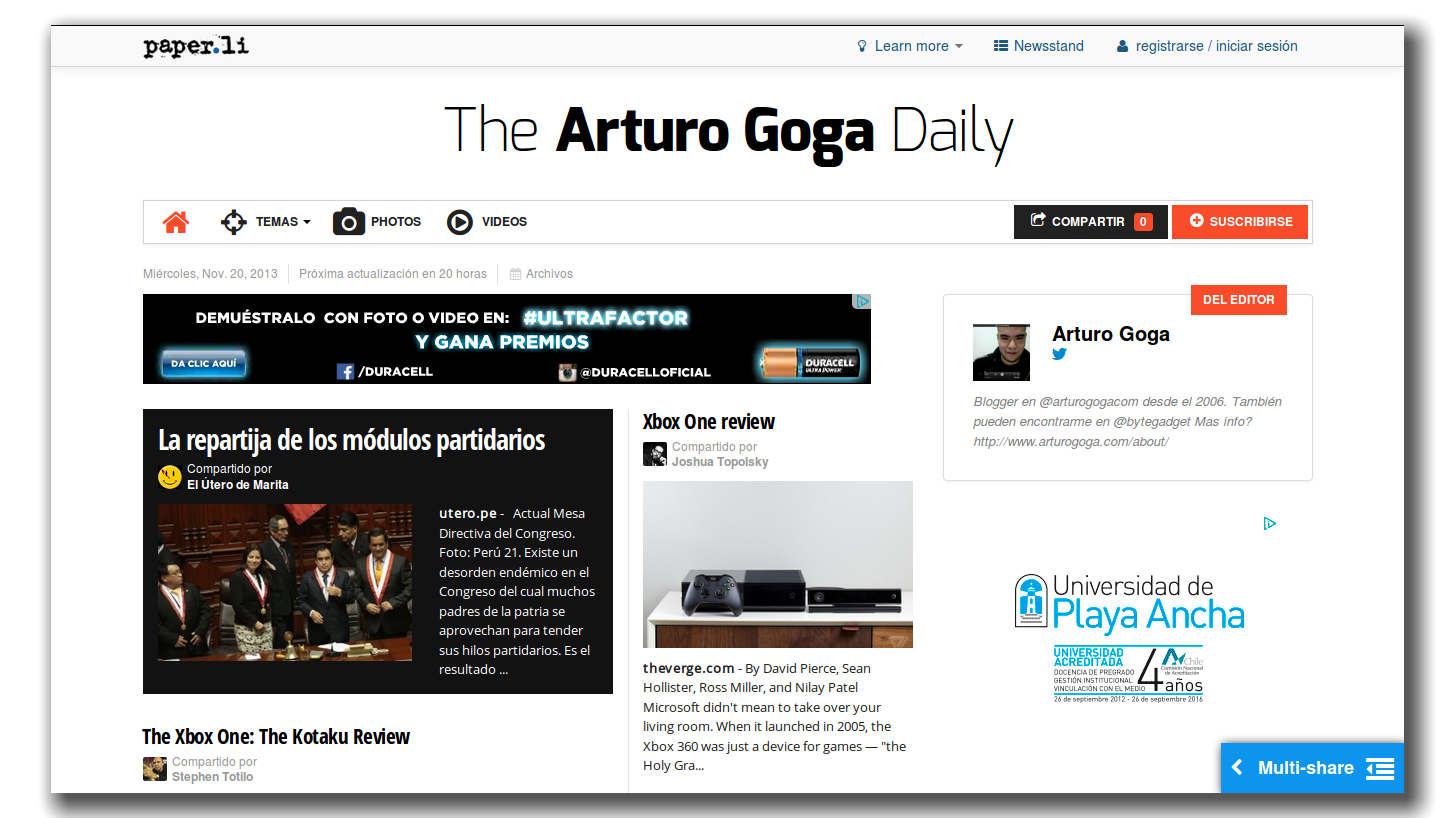
\epsfig{file=imgs/paperli1.png, width=2.5in} 
			\caption{Vista principal del periodico Paper.li de un usuario de la plataforma}
			\label{fig:paperli1}
		\end{center}
	\end{minipage}
	\hfill
	\begin{minipage}[t]{.45\textwidth}
		\begin{center}
			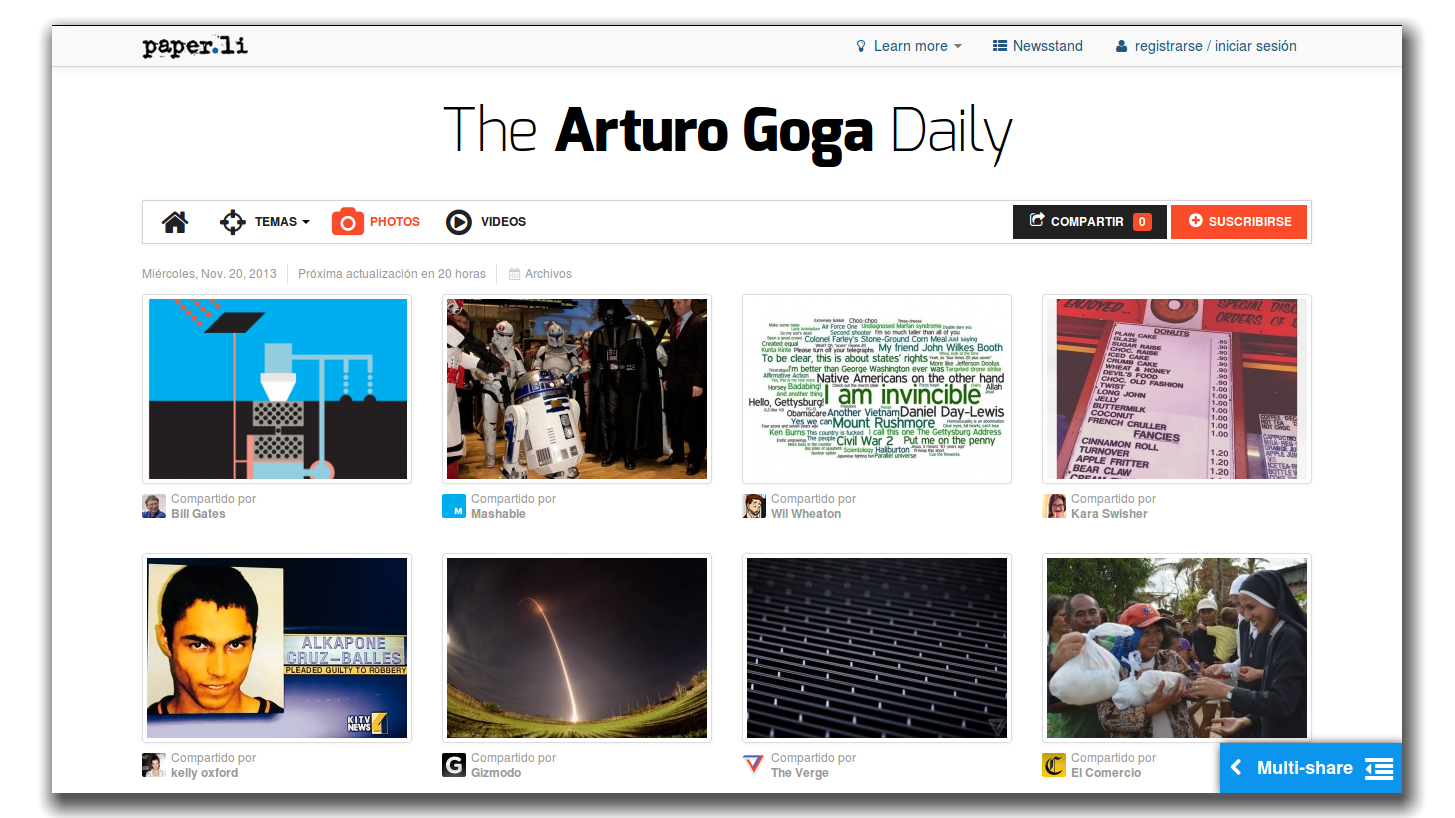
\epsfig{file=imgs/paperli2.png, width=2.5in} 
			\caption{Vista de fotografías del periodico Paper.li de un usuario de la plataforma}
			\label{fig:paperli2}
		\end{center}
	\end{minipage}
	\hfill
\end{figure}


\subsection{The Tweeted Times}

The Tweeted Times \cite{tweetedtimes} es una aplicación web lanzada en 2010 y desarrollada por Flipboard, Inc. permite generar en base a los \emph{feeds} recibidos en la cuenta de twitter, una especie de periódico de noticias con las temáticas más importantes, de forma similar a Paper.li \ref{subsec:paperli} pero sólo enfocado en Twitter y con la potencialidad de que se actualiza cada una hora.

The Tweeted Times posee otras potencialidades como su capacidad de personalización en la selección de los contenidos.
Además de la cuenta del mismo usuario, es posible crear periódicos con listas particulares de Twitter, con perfiles de usuarios, y hasta de una búsqueda de un hashtag o de usuarios.

The Tweeted Times usa un algoritmo particular para poder organizar las publicaciones de acuerdo con su correspondiente relevancia. El algoritmo se basa principalmente en la repercusión de dichas publicaciones en Twitter (cantidad de retweet, número de marcaciones como publicación favorita).

A cada enlace compartido se le asigna el valor de un \emph{ranking} relacionado con la cantidad de replicaciones por amigos y por amigos de amigos y menciona por cual de los contactos fue aportado el enlace. Permite explorar los periódicos de otros contactos en Twitter y también periódicos de otros usuarios destacados de la plataforma.

\begin{figure}[H]
	\centering
	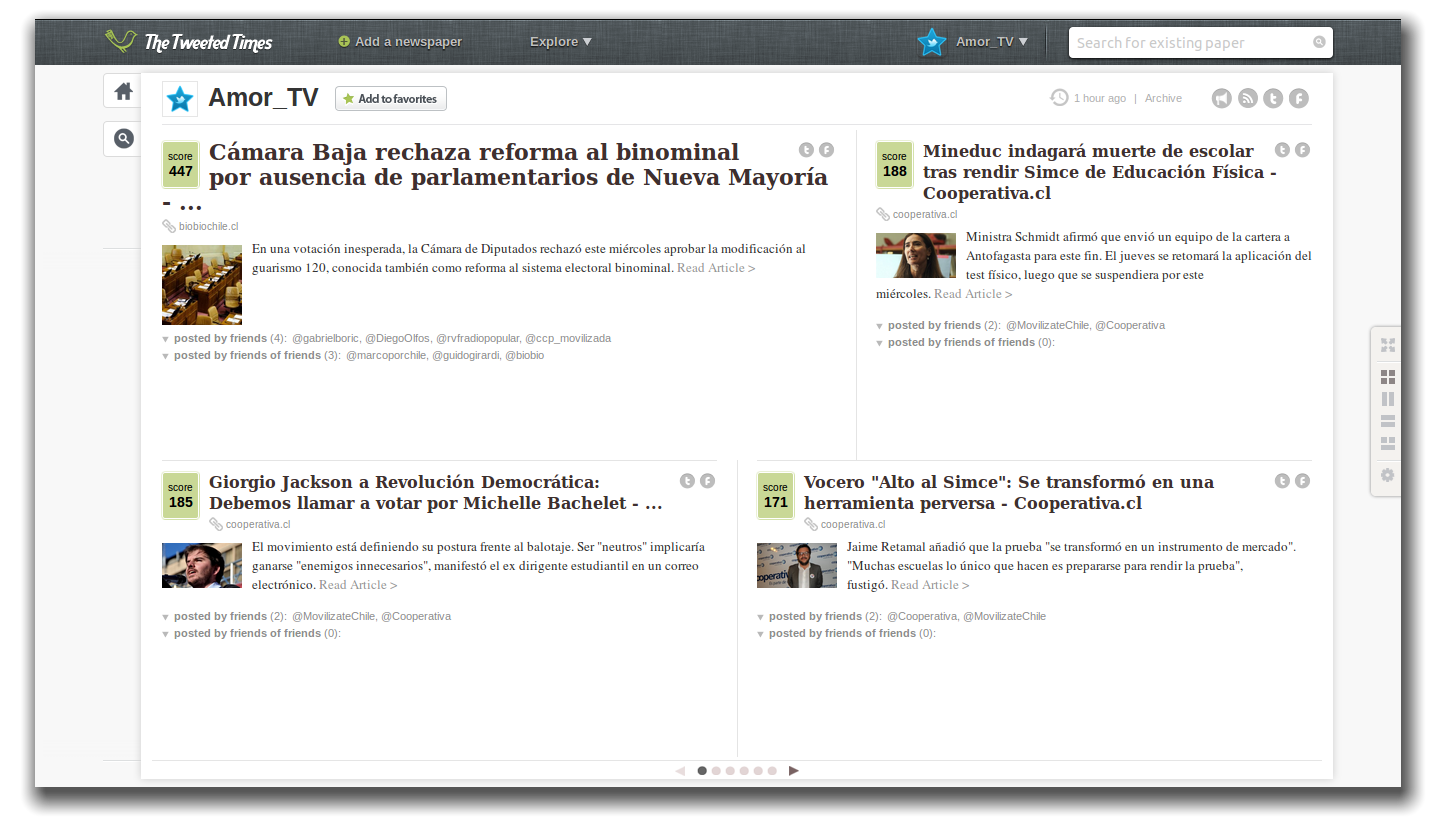
\includegraphics[width=0.8\textwidth]{imgs/tweettimes.png}
	\caption{Vista principal de un periodico creado en The Tweeted Times}
	\label{fig:tweetedTime}
\end{figure}

\subsection{FlipBoard}

Flipboard \cite{flipboard} es una aplicación lanzada en julio de 2010 que permite reunir las noticias del mundo y las novedades de las redes sociales en una revista diseñada para dispositivos móviles. El usuario puede elegir algunas temáticas y Flipboard crea una revista digital, en la cual se pueden ``hojear" las noticias de interés, así como las historias y fotos que los contactos del usuario compartan. Flipboard posee además una función que permite guardar artículos para verlos posteriormente o recopilarlos en ``revistas" propias de Flipboard.

%Flipboard promociona sus pontencialidades de la siguiente manera: ``Muévete a través de las noticias desde tu Twitter y publicaciones como la BBC, USA Today y The Verge. Entérate de todo, desde las fotos y mensajes compartidos por tus amigos en Facebook e Instagram, hasta los videos de YouTube y las novedades de la cultura pop de la revista Rolling Stone. Encuentra inspiración para tus viajes, moda y vida en sitios como la National Geographic, Elle España, Oprah y Cool Hunting. O crea tus propias revistas sobre cualquier tema, desde culinaria hasta Química". 
%https://play.google.com/store/apps/details?id=flipboard.app&hl=es_419

Flipboard actualmente permite la conexión con 12 redes sociales entre las que se incluyen Twitter, Facebook, Instagram, Google+, YouTube, Google Reader, LinkedIn, Flickr, 500px, Sina Weibo y Renren, en las cuales es posible realizar búsquedas mediante temas, hashtag, blogs y personas. Hoy en día existen 15 diferentes versiones de Flipboard entre países de América, Europa y Asia.

Flipboard también pone a disposición de sus usuarios contenidos seleccionados donde se incluyen las revistas y blog recomendados, fotografías y secciones especiales a noticias del día y temas de interés.

\begin{figure}[H]
	\centering
	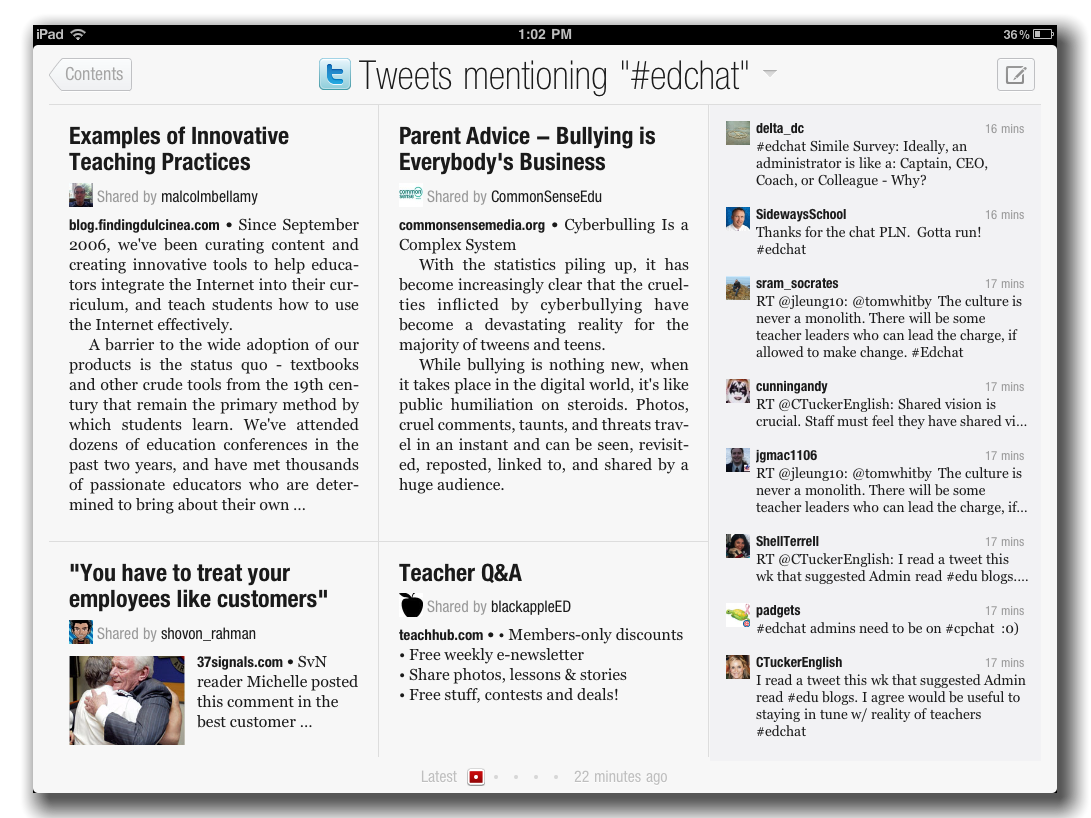
\includegraphics[width=0.8\textwidth]{imgs/flipboard3.PNG}
	\caption{Vista del formato de revista en Flipboard para visualizar los feeds de Twitter, donde se resaltan los tweet que han tenido mayor repercusión en la red y los enlaces compartidos}
	\label{fig:flipboard1}
\end{figure}

\subsection{Summify}

Summify\cite{summify} consistía en un servicio gratuito que permitía informarse de la actualidad por medio de recopilaciones diarias de las noticias que más circulaban entre el círculo de contactos de Twitter y Facebook, la cuenta de Google Reader o feeds RSS del usuario. Summify cesó sus funciones el 22 de junio de 2012 por decisión de Twitter a solo cinco meses de comprarlo. Summify entregaba su servicio de distintas formas: mediante la web para revisar las recopilaciones, vía correo electrónico, mediante la notificación por DM de Twitter cuando existe una nueva disponible y mediante la aplicación móvil.

La principal motivación para esta aplicación era expresada mediante su video promocional: En un inicio mantenerse al tanto de las actividades sociales es muy gratificante, pero luego, fácilmente, se puede convertir en una actividad agobiante y poco productiva por la gran cantidad de contactos y las diversas redes sociales existentes. Summify se presentaba como una alternativa productiva para mantener satisfactoriamente los vinculos sociales en la red.

Summify permitía la configuración de la cantidad de recopilación se deseaba recibir el usuario (de una a cuatro diarias) y a la hora de recopilación de la primera de éstas (las restantes se realizaban en consecusión en horas), era posible especificar la cantidad de artículos que poseían dichas recopilaciones (de dos a quince artículos), además de la privacidad de dichas recopilaciones (públicas o privadas). Su algoritmo se encargaba de recopilar los enlaces a artículos que aparecen en las cuentas del usuario en Twitter y Facebook y los filtraba en base a cuanto han sido compartidos, marcados con “Me gusta” o re-tweeteados, prestando atención a las personas con las que el usuario interactua más. También el algoritmo consideraba que tanto se ha compartido un enlace a nivel global, pero según indicaban en su blog de documentación, tenía menos relevancia que las interacciones del usuario con sus contactos. Otra cualidad del algoritmo que se utilizaba es que aprendía en base al uso dado por el usuario, analizando las tendencias y preferencias de uso, observando si se pinchaban más historias de un usuario en particular, en las de un dominio en concreto, en las que contienen unas palabras claves concretas dentro del título o cúal es la fuente de feeds más utilizada.

Cada recopilación poseía su propia página individual y mostraba las noticias seleccionadas una debajo de la otra. Junto a ellas, se visualizaban algunos de los usuarios que las habian compartido y al posicionar el puntero por encima de los avatares, el mensaje en el cual compartieron el artículo. Todas las recopilaciones se conservaban y eran posible acceder a ellas desde el perfil del usuario.

En el caso de que algunos de los contactos del usuario en Twitter y Facebook también estén usando Summify, era posible acceder a sus recopilaciones (en el caso de que éstas fuesen públicas). Era posible también navegar por los perfiles y recopilaciones de los usuarios que se siguen, que siguen al propio usuario y, además, de los que se considera que influencian al usuario y a los que influencian al usuario (es decir, que aparecen más veces en los resúmenes del usuario o en los que aparecemos más veces el propio usuario).


\begin{figure}[H]
  \centering
    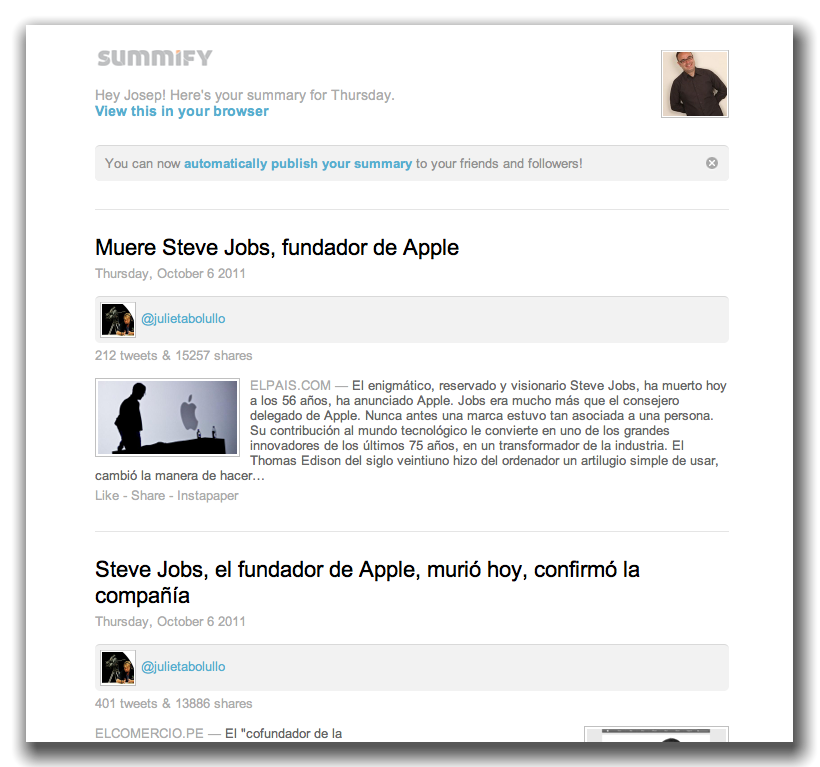
\includegraphics[width=0.8\textwidth]{imgs/summify.png}
  \caption{Vista de la recopilación de Summify}
  \label{fig:summify}
\end{figure}

\subsection{TwitterFall}

Twitterfall \cite{twitterfall} es un cliente web basado para Twitter que permite realizar búsquedas avanzadas y seguimiento de temas de tendencia. Fue construida el 2009 por Tom Brearley y David Somers, dos estudiantes de ciencias de la computación de 19 años en la Universidad de York y despúes de tres años de funcionamiento ha sido denominado como ``el google para la tweet-osfera".

El nombre de la plataforma se relaciona con la forma de su interfaz, ya que se presenta como una cascada de tweets que van cayendo hacia abajo de la pantalla a medida que existen nuevas actualizaciones en tiempo real tal como se pued ver en la figura \ref{fig:twitterfall}. La velocidad de este flujo puede ser personalizada mediante un simple ajuste.

Las potencialidades de TwitterFall radican en sus herramientas de búsqueda, entre las cuales se encuentran:
\begin{itemize}
	\item Realizar búsquedas mediante palabras claves o trendic topic.
	\item Focalizar búsquedas geolocalizadamente.
	\item Se puede realizar filtrados por idioma y excluir re-tweet.
	\item Permite almacenar las búsquedas favoritas.
\end{itemize}

TwitterFall permite también iniciar sesión en Twitter desde su interfaz y utilizarlo como clinte regular de Twitter y utilizarlo para responder mensajes, realizar re-tweet, seguir a nuevas personas, etc. otorga además interesantes características como pre-visualizaciones en ventanas flotantes sobre el enlace contenidos en tweets (sin necesidad de ser redirido a ellos), o  tras posicionar el puntero sobre un tweet se obtiene información sobre su ubicación y sus seguidores.

%TwitterFall también permite una gran cantidad de opcionees de presentación, como la personalización del tamaño de la fuente, el color, acelerar o disminuir la velocidad de refresco de la cascada de tweets. 

\begin{figure}[H]
	\centering
	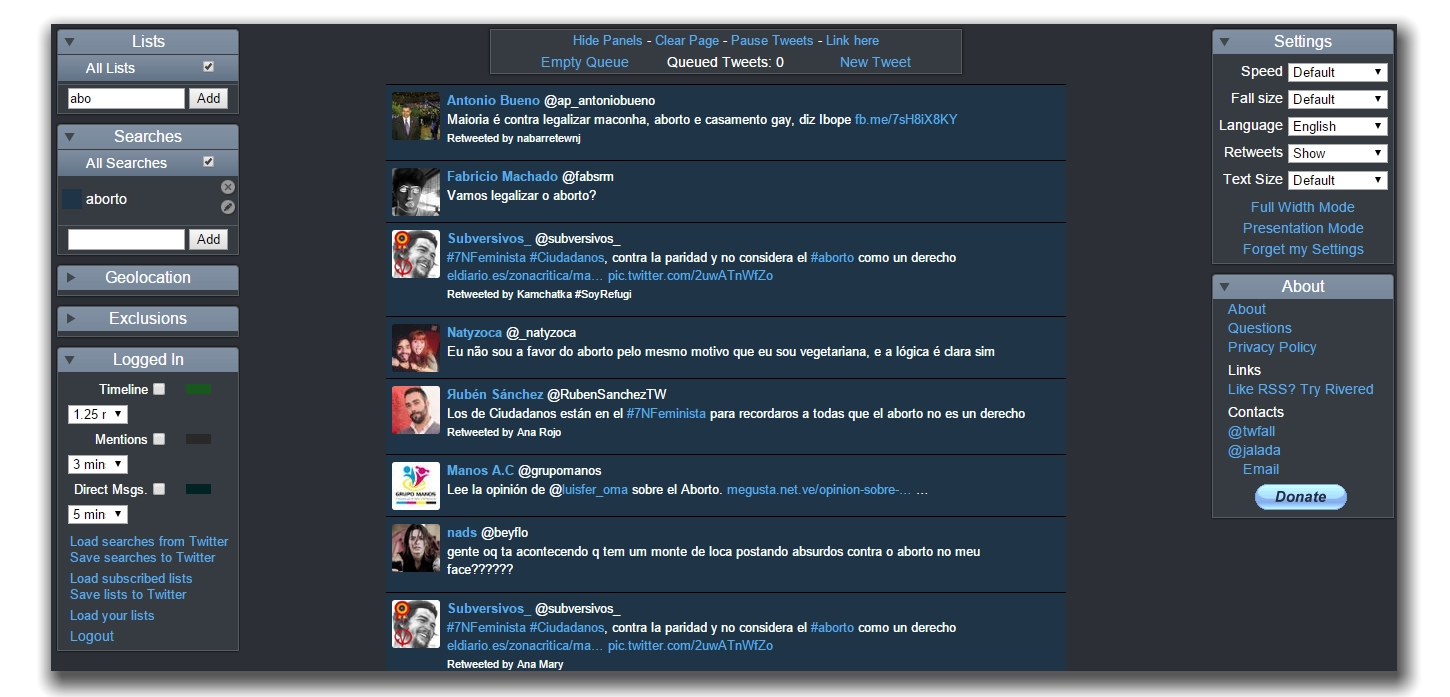
\includegraphics[width=0.8\textwidth]{imgs/twitterfall.jpg}
	\caption{Vista de la recopilación de Twitterfall}
	\label{fig:twitterfall}
\end{figure}

\subsection{Storyful}

\begin{figure}[h]
	\centering
	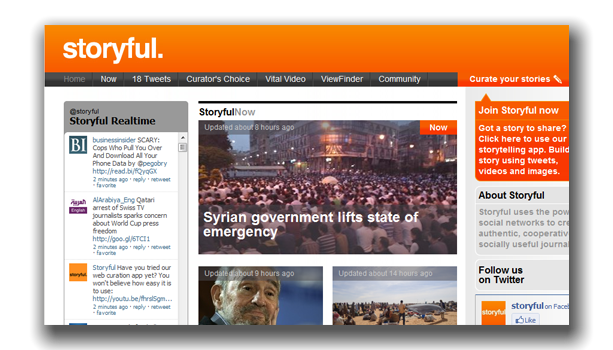
\includegraphics[width=0.8\textwidth]{imgs/storyful.png}
	\caption{Vista principal de Storyful}
	\label{fig:storyful}
\end{figure}

Fundada en Dublín con sólo tres empleados, Storyful \cite{storyful} tiene su razón de ser en idear una manera de administrar las enormes cantidades de contenido que se comparten en las redes sociales por millones de usuarios en todo el planeta, aplicando procesos y tecnología eficaz para ayudar a filtrar ``noticias de ruido". 

%Definiendo su servicio como ``Storyful es la primera agencia de noticias de la era de los medios sociales. Ayudamos a las salas de redacción a encontrar el contenido más valioso en la web social." \footnote{\url{http://storyful.com/about/}}. 

A finales del 2011 Storyful formó una alianza con YouTube para encontrar y la validar los vídeos que surgieron a partir de las protestas crecientes en Egipto.

Storyful pretende dotar de herramientas a todos los medios de prensa que las demanden, tal como declaran mediante su página web ``Desde 2010, Storyful ha estado construyendo y perfeccionando la primera sala de prensa verdaderamente social. Hemos perfeccionado nuestras técnicas, herramientas y servicios, en colaboración con algunas de las marcas más importantes de noticias en el mundo, incluyendo ABC News, Reuters y el New York Times, y plataformas sociales como YouTube.

Storyful ha desarrollado lo que llaman como ``algoritmo humano" que consiste en un conjunto de procesos algorítmicos y humanos que posee gran aceptación hoy en el mercado de las noticias obtenidas de medios sociales. 
%uestra ambición es ayudar a cada organización de noticias a construir su propia sala de redacción social. Queremos equipar a todos los periodistas con las habilidades y herramientas necesarias para aceptar el cambio. Queremos ayudar a los editores y locutores construir productos que realizan las audiencias y ganar dinero. "

Para los nuevos medios sociales Storyful plantea que los periodistas deben pensar en su papel en un mundo cambiante, comenzando a utilizar nuevas herramientas inteligentes y rápida, complementándolas con los conocimientos profesionales y de oficio de los periodistas. Separando el proceso en tres etapas: descubrimiento de hechos noticiosos, verificación y entrega o presentación de los contenidos.

Storyful asegura que la única manera de verificar una información y restringir correctamente su ruido es unirse a la conversación sostenida en los medios sociales desde donde surgen los hechos noticiosos aprovechando las oportunidades que ofrecen hoy en día las tecnologías actuales, pero no sólo escuchar en ellos, sino participar directamente, de forma abierta y honesta con las voces más cercanamente relacionadas con el hecho. Esta es una clave del algoritmo humano "La mayoría de las organizaciones de noticias se busque en observadores pasivos. Pero eso no es suficiente. La única manera de desbloquear el poder de la Algoritmo humano es ser una parte de ella"\footnote{\url{http://storyful.com/about/}}.

Señalan que el valor de la información al relacionarse en los grupos de redes sociales es increíble, apasionante y de rápida evolución, pudiendo explicitar relaciones con otros hechos noticios aparentemente invisibles, que finalmente enriquecen la noticia y la completan, permitiendo contacto y conversaciones abiertas, informadas y sinceras con los lugareños del mismo sector o con acádemicos de la zona, con información que de otro modo dificilmente fuese recolectada.

Storyful plantea que fue diseñado para ``vivir dentro de las comunidades de medios sociales, no para observar desde una distancia segura". Para lo cual cuenta con jueces en terreno que establecen vínculos sociales y contactos con personas del entorno para acreditar desde estas relaciones, la veracidad de la información, complementando el proceso de verificación establecido para un hecho en específico.

El proceso de verificación es la piedra angular del proceso, puesto que muchas veces en las redes sociales se hacen circular deliberadamente informaciones incorrectas, generando desinformación y percepciones erradas. En dicho proceso aplican las siguientes preguntas para generar un cierto nivel de fidelidad de la información aportada por un cargador en Youtube:

\begin{itemize}
	\item ¿Dónde se ha registrado esta cuenta y en que se ha basado el autor para emitir su juicio de la historia?
	\item ¿Existen otras cuentas en Twitter, Facebook, blogs o sitios web relacionados a este autor ? ¿Qué información tienen para indicar la ubicación reciente, la actividad, la fiabilidad y/o el sesgo?
	\item ¿Hace cuánto tiempo existen esas cuentas? ¿Qué tan activas son?
	\item ¿La narración del contenido se escribe en jerga o dialecto identificable en la narración de la publicación?.
	\item ¿Podemos encontrar información WHOIS\footnote{Es un protocolo de petición y respuesta ampliamente utilizado en bases de datos para el registro de usuarios o asignaciones de algun recurso de Internet, como el nombre del dominio o el bloque de dirección IP} para algún sitio web afiliado ?
	\item ¿El cargador aparece en los directorios locales ? ¿Qué indican sus círculos sociales en línea que están cerca de esta historia / ubicación?
	\item ¿Tiende el cargador a 'copiar' contenidos de otras cuentas de Youtube , o carga únicamente contenido generado por el usuario?
	\item ¿Los videos de la cuenta del cargador tienen una calidad consistente?
	\item ¿La descripción del video es consistente y señalan un lugar específico ? ¿Corresponde la fecha? ¿Tiene la extensión de archivo como AVI o MP4 en el título del video?
	\item ¿Storyful esta familiarizado con esta cuenta? ¿su contenido ha sido fiable en el pasado?
\end{itemize}

Storyful comparte sus conocimientos y técnicas de forma abierta desde el blog de su plataforma los cuales se revisan a continuación debido a su posible aplicabilidad como directrices en este trabajo:

\begin{itemize}
	\item{\textbf{Hacer listas: Cómo afinar sus antenas Twitter}} \cite{storyfulblog}
	
	Una herramienta fundamental para el funcionamiento de Storyful, son las listas temáticas de Twitter. Debido al amplio flujo de información en la era de los medios sociales, las listas funcionan como el filtro perfecto de noticias en vivo, permitiendo afinar el lugar de observación, un objeto o un evento y silenciar algunas conversaciones no útiles que tienen lugar simultáneamente.
	
	Manejan simultáneamente cientos de listas de Twitter que cubren todos los países del mundo y todos los temas imaginables es complejo. 
	
	Para la administración de estas listas se utiliza la herramienta \emph{Tweetdeck}\cite{tweetdeck}, donde a cada terminal se le cargan cerca de 20 a 30 listas para ser visualizadas por un periodista. \emph{Tweetdeck} es utilizado (a pesar de sus limitantes en el número de listas que permite por usuario) por las facilidades de gestión que aporta como la agrupación y orden dinámico de las listas por temáticas similares, clasificación e inclusión de nuevos elementos (como usuarios o tópicos) mediante mecanismos interactivos.
	
	%Listas de Twitter ayudan a trazar sus miembros y canalizar su información en "tiempo real" , el debate y la verificación. 
	
	\item {\textbf{Verificación de videos}} \cite{storyfulblogvideos}
	
	\begin{itemize}
		\item Revisión de la historia y la ubicación del cargador para ver si ha compartido contenido útil y creíble en el pasado.
		\item Uso de las imágenes Google Street View para ayudar a verificar los lugares en un video.
		\item Consulta de otras fuentes de noticias o contenido de usuario validado para confirmar eventos ocurridos en el video.
		\item Examinar características claves del video como el clima y el paisaje de fondo para ver si coinciden con los hechos conocidos en terreno.
		\item Traducción de toda palabra que sale en el vídeo a modo de contexto adicional.
		\item Supervisar el tráfico de las redes sociales para ver quién está compartiendo el contenido y qué preguntas se les pide al respecto.
		\item Desarrollar y mantener relaciones con las personas dentro de la comunidad alrededor de la historia.
	\end{itemize}
	
\end{itemize}

\subsection{Wikipulse}

Wikipulse es un medio de prensa \cite{Futterer:arXiv1308.1166} basado en el hecho de que la basta comunidad de editores de Wikipedia muchas veces logran actualizar este portal y anunciar un hecho, mucho antes que los medios de prensa convencionales. Wikipulse recoge las más recientes ediciones y las presenta en un formato ordenado y simple.

Existen estudios \cite{wikipediaEditor:Online} que verifican que existen muchos editores en Wikipedia que se encargan de actualizar lo más pronto posible diversos los artículos, motivados por la mejora en su reputación como publicadores que esto implica, dichas actualizaciones llegan incluso a hacerse públicas en un tiempo promedio de dos horas inferior al reporte de noticieros como CNN o \emph{Reuters online} \cite{beckerWikipedia}.

Wikipulse realiza su trabajo en tres principales tareas:
\begin{enumerate}
	\item Encontrar artículos relevantes en Wikipedia
	\item Reformar los artículos en formato de noticias
	\item Mostrarlos en una página web
\end{enumerate}

El núcleo como tal de Wikipulse esta compuesto por dos componentes: Wikipedia actúa como fuente principal de artículos de noticias mediante artículos editados o publicados por al comunidad de Wikipedia, y la segunda componente esta compuesta por la generación de noticias de Wikipulse de forma automática obtenidos desde Wikipedia agrupados en las distintas categorías (eventos corrientes, deporte, etc.).

Para el criterio de selección además del criterio obvio de los artículos editados más recientemente en Wikipedia, se emplea un algoritmo planteado en un trabajo reciente en \cite{journals/corr/abs-1204-3375} se observa que en la edición de un artículo se genera una red basada en vínculos de ``editores-compartidos": dos artículos diferentes tienen un vínculo entre ellos si el mismo editor modifica ambos

La selección de los autores ``correctos" garantiza artículos de interés periodístico por el mantenimiento de una lista cada vez mayor de editores frecuentes que se centran en el artículo-tipo de prensa. La comprobación de si los hechos del artículo son verídicos ocurre de forma gratuita a través del principio de los muchos globos oculares de Wikipedia (muchos usuarios ven y corroboran si la información es verídica, si no lo es, la editan).

En el segundo paso se formatean los artículos de Wikipedia a un estilo más periodístico, usando técnicas automática de generación abstracta. El paso final consiste en mostrar las artículos en un formato periódico de manera online.

El sistema se encuentra conformado por cuatro capas: Wikipedia, La capa de extracción, la capa de selección de noticias y la página de presentación.\\
\textbf{Algoritmo de selección de noticias} \\
El algoritmo se basa en tres grandes etapas: 

\begin{enumerate}
	\item \textbf{Creación del Conjunto de trabajo}:
	El algoritmo es ejecutado periódicamente y en cada ejecución procesa un conjunto de noticias, las cuales son llamadas \emph{conjunto de trabajo}. Este \emph{conjunto de trabajo} contiene el conjunto de páginas recientemente editadas en Wikipedia. Cada una de estás páginas es pasada posteriormente por las otras componentes del algoritmo.
	En primer lugar la página de metadatos, el título y la totalidad de los autores y todas sus categorías son guardadas en una base de datos de un grafo de autores, permitiendo posteriormente a otras partes del algoritmo realizar consultas sobre esta información.
	El proceso de almacenamiento asegura que la base de datos es actualizada y expandida con cada ejecución del algoritmo aun cuando no existen nuevas noticias son generadas.	
	\item \textbf{Selección de Noticias}:
	El proceso de selección busca páginas de Wikipedia que podrían llegar a ser noticias posteriormente. Esto es mediante la generación. Esto se realiza mediante la generación de un ranking \emph{r} por cada página, éstos son comparados con un valor de umbral \emph{t}. Cada rank esta basado en consultas a la base de datos, ponderadas por un peso \emph{w} que especifica la importancia de ese rank en el resultado final. Una página genera una noticia cuando se cumple que:
	
	\begin{equation*}
	\sum_{i=1}^{n} {r_i \cdot w_i} > t_i
	\end{equation*}  
	
	Cada rank diferente que es generado por cada página son explicados a continuación. La mayor parte de ranks son ratios computados en orden para tener un conjunto predecible de números como resultado.
	\begin{itemize}
		\item Autor-con-Noticia
		el rank Autor-con-noticia aumenta la importancia de las páginas autores generadores-de-noticias(autores que ya han generado noticias). Y se calcula como la cantidad de autores que editan la página p partido por todos los autores generadores de noticias.
		
		\item Autores-comunes
		Calcula la popularidad de una página p mediante sus autores. Calculando el ratio de todos los autores editando la pagina p por todos los autores de la base de datos.
		
		\item Dominio-experto
		El rank dominio-experto identifica páginas importantes mediante el conteo del conjunto de expertos que editan la página. Un experto del dominio es aquel autor en Wikipedia que edita páginas en la misma categoría que la página que se esta evaluando.
		
		\item Cambios-recientes
		Este rank mide la actividad de edición en la página en comparación con todas las otras páginas del conjunto de trabajo.
		\item Relevancia
		La relevancia utiliza una evaluación de un webservice externo para determinar la popularidad de una página de Wikipedia.	
	\end{itemize}
	\item \textbf{Creación de noticias}:
	El proceso de creación de noticias crea noticias a partir de las páginas. Esto se hace mediante el análisis y la agregación de las ediciones de una página en una gran bloque de texto, que se envía a continuación a un webservice llamado \emph{summry.com} que las resume en un artículo de noticias cortas. Este articulo de noticia es guardado en la base de datos, y se presenta a través de la interfaz web.
	Para agregar una edición, esta es elegida en base a tres criterios:
	\begin{itemize}
		\item La edición debe ser hecha por un editor top.
		\item La edición debe ser hecha por un experto del dominio.
		\item La edición es más larga que 50 caracteres.
	\end{itemize}
	Un editor top es aquel autor que esta dentro de los ``editores top" lista que incluye los autores y expertos de dominio que tienen más ediciones para una categoría dada.
\end{enumerate}

\textbf{Capa de extracción}\\
Es la capa encargada de mediante una conexión a la API de Wikipedia permite el acceso a las páginas modificadas y sus datos
respectivos.
Esta capa utiliza algunas herramientas externas:
\begin{itemize}
	\item smmry.com una API abierta que permite resumir textos de páginas con un número excesivo de oraciones. (Disponible en http://smmry.com/api ).
	\item stats.grok.se un subproyecto de Wikipedia el cual mantiene estadísticas de las diversas páginas de Wikipedia.
\end{itemize} 

\textbf{Análisis de los datos} \\
El análisis de datos se realizó con intenciones de medir el rendimiento del seleccionador de noticias, de esta forma se decidió compararlo con algunas fuentes de información tradicionales como (CNN, Reuters, etc.) La idea principal es comprobar si las noticias seleccionadas por Wikipulse también fueron registrados como noticias por los medios de comunicación convencionales (dentro de un límite determinado de tiempo). Para dicha medición se utilizaron los siguientes criterios:

\begin{itemize}
	\item Precisión y relevancia
	Medida del solapamiento entre las noticias de Wikipulse y las reporteadas por los medios tradicionales en algun tiempo dado.
	\item Frescura/rapidez
	Criterio que mide el tiempo relativo respecto al solapamiento de las noticias entre Wikipulse y los medios convencionales. Este indica si Wikipulse es más rápido o mas lento en términos de reporte.
\end{itemize}

Para comparar los resultados de Wikipulse se compararon los reportes con un medio convencional mediante el acceso a su RSS y así obtener el momento de inicio en la difusión de la noticia. Para comparar si se trataban del mismo contenido, se realizó un proceso de \emph{match} entre ambos recursos de la siguiente manera: Las historias individuales obtenidas de ambos \emph{feeds} son procesados para obtener una lista de palabras. Los distintos artículos de ambos feed son comparados mediante el \emph{match} de las palabras claves. El cuantificador se calcula mediante una fracción entre el número total de match encontrados partido por el número total de \emph{keywords} en cada uno de los artículos. Empíricamente se encontró que un cuantificador superior a 0.33 generalmente indicaba un \emph{match} fuerte.

	
	%\input{estadoDelArte.tex}	
	\chapter{Definición de la solución}\label{chap:contexto}
	Existe un creciente desconfianza por parte de la ciudadanía respecto a la repercusiones reales del proceso de \emph{gatekeeping} en las noticias publicadas por los medios de prensa tradicionales.

La irrupción de Internet y las redes sociales en la vida cotidiana han modificado variados esquemas de comunicación y formas de relación
entre las personas, entre ellos, los medios de prensa y la forma que tienen las y los ciudadanos para informarse de los eventos que ocurren en su entorno. Tambini en  \footnote{http://wallblog.co.uk/2013/03/05/how-twitter-won-the-social-media-battle-for-journalism/\#ixzz2kBQ2RFcQ } señala ``El papel de \emph{gatekeeper} de los medios de prensa tradicionales se ha debilitado y las personas construyen su propia estructura editorial eligiendo que siguen en los medios de comunicación basados en la recomendación. Las redes sociales también difieren en el sentido de que tienen un compromiso con la universalidad y apertura, que es más importante para ellos que los periódicos estén ahí" 

Twitter debido a las múltiples características que posee referente a su capacidad de propagación, acceso y espontaneidad se presenta como una importante red social que hoy revoluciona la industria periodística mundial, obligando a las grandes cadenas a integrarles dentro de su proceso periodística. Hughes, un corresponsal muy influyente y famoso de la BBC, dice: ``Los medios sociales permiten que consiga mucho más acerca de la historia. Hay periodistas y otras personas en el mismo lugar del suceso que reportan los eventos en tiempo real, de manera que cuando una historia en realidad aparece en la televisión, a menudo ya la he visto través de los medios sociales". Hughes declara, que al igual que una gran cantidad de periodistas, recolecta inicialmente una gran cantidad de noticias desde Twitter. Otros informes dicen que la cifra de periodistas recibiendo historias y eventos de Twitter es de aproximadamente 50\%. Hughes dice que el 80\% de su recopilación de noticias la obtiene en Twitter y sólo el 20\% de otras fuentes \cite{RePEc:ehl:lserod:59881}.

Considerando el interés creciente de adquirir información de eventos noticiosos desde sus fuentes directas evitando los procesos de \emph{gatekeeper} sumado a las potencialidades que posee Twitter referente a esta misma temática se busca diseñar e implementar una herramienta que permita comunicar los reportes en Twitter de un determinando evento, privilegiando aquellos reportes con menor cantidad de intermediadores y posibles \emph{gatekeeper}, siendo estos, las y los observadores y las y los reportadores directos del suceso.

\section{Objetivos}

\subsection{Objetivo principal}

\begin{itemize}
\item Desarrollar un algoritmo computacional que permita recoger tweets que reporten un evento, priorizando 
los tweets geolocalizados cercano al lugar de ocurrencia del evento, para generar un relato temporal
referente a dicho evento que será presentado mediante una interfaz web.
\end{itemize}

\subsection{Objetivos Secundarios}
\begin{itemize}
\item Analizar trabajos previos y herramientas creadas con anterioridad para encontrar la forma adecuada y más conveniente de proceder a la construcción de esta herramienta.
\item Dotar al público interesado en informarse sobre eventos noticiosos de una herramienta de reporte de eventos que minimiza el filtrado y tratamiento editorial de contenidos.
\item Desarrollar una interfaz web que sea clara y fácil de usar por el usuario.
\end{itemize}

	\chapter{Propuesta}\label{chap:propuesta_cap}
	\section{Arquitectura de la solución}
	La Arquitectura de la solución se compone de los siguientes macroprocesos conceptuales: 

\begin{itemize}
	\item Captura de datos: Captación de usuarios y captación de tweets.
	\item Almacenamiento.
	\item Procesamiento de tweets: Extracción de datos e Indexación de datos.
	\item Presentación de los datos.
\end{itemize}


	
	\begin{figure}[H]
	\centering
\begin{tikzpicture}[node distance = 2cm, auto,
database/.style={
	cylinder,
	cylinder uses custom fill,
	cylinder body fill=yellow!50,
	cylinder end fill=yellow!50,
	shape border rotate=90,
	aspect=0.25,
	minimum height=4em,
	draw
}
]
% Place nodes
%\node [] (i1) {t};
\node [draw, fill=gray!20 ,cloud, cloud puffs = 10, minimum width=1cm, minimum height=0.75cm, node distance=3cm](i1){Twitter};
\node [block, below left of=i1, node distance=3.5cm] (i2) {\textsf{Captura de usuarios}};
\node [block, below right of=i1, node distance=3.5cm] (i3) {\textsf{Captura de tweets}};
\node [database, below of=i1, node distance=5cm] (i4) {\textsf{Base de datos}};
\node [block, below left of=i4, node distance=2.5cm] (i5) {\textsf{Extracci{\'o}n de datos}};
\node [state, right of=i5, node distance=4cm] (i6) {\textsf{Ingreso t{\'o}pico}};
\node [block, below of=i5, node distance=2.5cm] (i7) {\textsf{Indexaci{\'o}n de datos}};
\node [block, right of=i7, node distance=4cm, minimum width=2.5cm] (i8) {\textsf{Presentaci{\'o}n t{\'o}pico}};

\begin{scope}[on background layer]
\node[rectangle,draw,minimum width=6cm] [fit = (i2) (i3),fill=yellow!20,rounded corners, draw=black!50, dashed, label=right:Captura de datos] (bx4) {};
\end{scope}

\begin{scope}[on background layer]
\node[rectangle,draw,minimum width=3.5cm] [fit = (i5) (i7),fill=yellow!20,rounded corners, draw=black!50, dashed, label=below:Procesamiento de tweets] (bx4) {};
\end{scope}

\begin{scope}[on background layer]
\node[rectangle,draw,minimum width=3cm] [fit = (i4),fill=yellow!20,rounded corners, draw=black!50, dashed, label=right:Almacenamiento] (bx4) {};
\end{scope}

\begin{scope}[on background layer]
\node[rectangle,draw,minimum width=3cm] [fit = (i6)(i8),fill=yellow!20,rounded corners, draw=black!50, dashed, label=below:Presentacion de datos] (bx4) {};
\end{scope}

%\node [decision, below of=i2, node distance=3cm] (i3) {\textsf{keyIn}($\mathbf{dt}$)};
%\node [state, below of=i3, node distance=3cm] (i4) {Se descarta t};
%\node [state, right of=i4, node distance=4cm] (i5) {saveLink(t)};

% Draw edges
\path [line] (i1) -- (i2);
\path [line] (i2) -- (i1);
\path [line] (i1) -- (i3);
\path [line] (i3) -- (i1);
\path [line] (i2) -- (i4);
\path [line] (i3) -- (i4);
\path [line] (i4) -- (i5);
\path [line] (i5) -- (i4);
\path [line] (i5) -- (i7);
\path [line] (i6) -- (i5);
\path [line] (i7) -- (i8);
%\path [line] (i2) -- node [near start] {dt}(i3);
%\path [line] (i3) -- node [near start] {no}(i4);
%\path [line] (i3) -| node [near start] {si}(i5);
\end{tikzpicture}
\caption{Diagrama conceptual de la arquitectura de la solución} \label{fig:dia-arquitectura-sw}
\end{figure}
	
\section{Plataformas y herramientas utilizadas}

	Las plataformas y herramientas utilizadas para desarrollar el prototipo fueron las siguientes:

\begin{itemize}
	\item \textbf{Python}
		
		Python es un lenguaje interpretado de programación orientado a objetos con una sintaxis muy clara. Incorpora módulos, excepciones, interpretación dinámica y tipos de datos dinámicos de muy alto nivel, posee además variadas interfaces para muchas llamadas de sistema y bibliotecas así como de sistemas de ventanas y es extensible en C o C++. 
		
		%Según su propia página web \cite{pythonWeb} \emph{Python combina una notable potencia con una sintaxis muy clara. Tiene variadas interfaces para muchas llamadas de sistema y bibliotecas así como de sistemas de ventanas y es extensible en C o C++}. Otra cualidad notable de Python es que es portátil y se ejecuta en la gran mayoría de variantes de UNIX, Mac y Windows.
		
		Python cuenta actualmente con una gran comunidad que genera y mantiene una robusta documentación lo que lo vuelve más accesible al aprendizaje. El lenguaje viene con una biblioteca estándar que cubre áreas como procesamiento de strings (expresiones regulares, unicode, diferencia de archivos), procotolos de internet (HTTP y FTP entre otros), ingeniería de software y las interfaces del sistema operativo (llamadas al sistema operativo y sistemas de archivos). Python cuenta también con una gran variedad de extesiones desarrolladas por terceros \cite{pythonPypiWeb}, algunas de las cuales fueron ocupadas en este trabajo.
		
	\item \textbf{Librerías de Python utilizadas}
		\begin{itemize}
			\item \textbf{LMXL}\label{itm:lxml}
			
			LMXL \cite{lxmlWebsite}  es un conjunto de herramientas que vinculan las librerías C libxslt2 y libxslt para su uso en Python, combinando la velocidad y la exhaustividad de las funciones para el análisis de XML de estas librerías con la simplicidad de Python.	Implementa los siguientes protocolos: \textit{XML 1.0},\textit{HTML 4}, \textit{XML namespaces}, \textit{XML Schema 1.0}, \textit{XPath 1.0},\textit{ XInclude 1.0}, \textit{XSLT 1.0}, \textit{EXSLT}, \textit{XML catalogs}, \textit{canonical XML}, \textit{RelaxNG}, \textit{xml:id}, \textit{xml:base}.		
			
			Posee una basta documentación debido a que implementa ElementTree API \cite{elementTree}. La librería se encuentra bajo licencia BSD. Mientras que las librerías que extiende libxml2 y libxslt2 permiten su uso bajo licencia MIT.
			
			\item \textbf{TextBlob}
			
			TextBlob \url{textblobWebsite} es una librería de Python para el procesamiento textual, posee una API simple para profundizar en las tareas  del procesamiento del lenguaje natural (NPL en inglés) como etiquetar partes de un discurso, análisis emocional y traducciones. La librería posee una basta documentación y su licencia de uso permite el acceso, edición y uso de manera gratuita.
			
			\item \textbf{Levenshtein}
			
			La extensión de Levenshtein \cite{pythonLeven} para Python es una extensión desarrollada en C que permite el fácil desarrollo de operaciones como: 
			\begin{itemize}
				\item Calcular la distancia de Levenshtein.
				\item Calcular la similitud de strings.
				\item Calcular la similitud de conjunto de strings.
			\end{itemize}
			
			Esta extensión posee licencia GNU.
		\end{itemize}

		
		\item \textbf{MySQL}
		
		MySQL \cite{mysqlWeb} es un sistema de gestión de bases de datos relacionales, multihebra y multiusuario con más de seis millones de instalaciones. MySQL AB desarrolla MySQL como software libre en un esquema dual bajo licencia GNU GPL y licencia de pago para productos privativos. MySQL destaca por su gran adaptación a diferentes entornos de desarrollo permitiendo su interacción con los lenguajes de programación más utilizados como PHP, Perl, Python y JAVA. 
		
		MySQL posee las características distintivas de otros motores de bases de datos:
		\begin{itemize}
			\item Permite escoger entre múltiples motores de almacenamiento para cada tabla (entre los que se encuentra MyISAM, Merge, InnoDB, Memoryheap y muchos más).
			\item Permite la agrupación de  transacciones para mejorar el número de transacciones por segundo.
		\end{itemize}
		
		Mysql actualmente es usado por muchos sitios web populares como Wikipedia, Google, Facebook, Twitter, Flickr y Youtube. 
		
	\item \textbf{Pycharm}
	
		Pycharm \cite{pycharmWeb} es una IDE utilizada para programar en Python. Esta IDE provee análisis de código, un \emph{debugger} gráfico, una unidad integrada para pruebas e integración con sistemas de control de versión además de soporte web para desarrollar con el framework Django. Algunas empresas que utilizan Pycharm son: Ebay, Groupon, Linkedin, Twitter, Spotify y HP. Pycharm cuenta con una licencia Profesional libre para proyectos de código libre y para fines educacionales, cuenta también con una edición \emph{community}.

	\item \textbf{Django}
	
	Django \cite{djangoWeb} es un framework de alto nivel de desarrollo web en Python que fomenta el desarrollo rápido y el diseño limpio y prágmatico. Django es gratuito y de código abierto y se basa en el patrón de arquitectura MVC.
	
	El objetivo principal de Django es facilitad el desarrollo de sitios web complejos con bases de datos. Django potencia la reutilización y conexión de componentes, el rápido desarrollo y el principio de no repetir código. Django ofrece también una herramienta administrativa opcional que mediante una interfaz web comúnmente utilizada por los administradores del sistema web para crear, modificar y leer los datos de la plataforma web en cuestión. 
	
	Las componentes de Django se basan principalmente en un modelo MVC, tratándose de un mapeador objeto-relacional que media entre los modelos de datos (definidos como clases de Python) y una base de datos relacional (llamado \emph{modelo}), un sistema para el procesamiento de las peticiones HTTOP con un sistema de plantillas web (llamados \emph{vistas}) y una despachador basado en expresiones regulares de URL (llamado \emph{Controlador}).
	
	Django soporta oficialmente cuatro bases de datos backend: PostgreSQL, MySQL, SQLite y Oracle.
	
	El framework también incluye:
	
	\begin{itemize}
		\item Un servidor web ligero y autónomo para el desarrollo y pruebas.
		\item Un formulario de serialización y un sistema de validación el cual puede traducir entre los formularios HTML y los valores esperables para el almacenamiento en la base de datos.
		\item Un sistema de plantillas que utiliza el concepto de herencia.
		\item Un sistema de internacionalización, incluyendo traducciones de propios componentes de Django en una variedad de idiomas.
	\end{itemize}
	
	Algunos sitios conocidos que utilizan Django son: Pinterest, Instagram, Mozilla y The Washington Times y cuenta actualmente con una activa comunidad de decena de miles de usuarios y colaboradores en todo el mundo.
	
	\item \textbf{Mysql Workbench}
	
	MysqlWorkbench \cite{mysqlWorkbenchWeb} es una herramienta visual de diseño de bases de datos que integra el desarrollo de SQL, administración, diseño, creación y mantenimiento de bases de datos en un único entorno de desarrollo integrado para MySQL.
	
	MySQL Workbench proporciona herramientas visuales para crear, ejecutar, y optimizar consultas SQL. El editor de SQL proporciona color resaltado de sintaxis, auto-completado, la reutilización de fragmentos de SQL y el historial de ejecución de SQL. El panel de conexiones de base de datos permite a los desarrolladores para gestionar fácilmente las conexiones de base de datos estándar, incluyendo Tela MySQL. El Examinador de objetos proporciona acceso instantáneo a esquema y objetos de base de datos.
	
	\item \textbf{Api de twitter}
	
	Twitter mediante sus API \cite{twitterWeb} habilita para que desarrolladores puedan escribir y leer en Twitter. Para el acceso y manipulación de datos de Twitter existen dos API disponibles: Rest API y Streaming API. La Rest API permite crear nuevos tweets, conocer información sobre el autor de un tweets entre otras acciones relacionadas a tweets o usuarios particulares. La Streaming API entrega un flujo constante de información en tiempo real.
	
	La Rest API de Twitter identifica aplicaciones mediante OAuth, posee una limitación de 150 solicitudes por hora cuya repercusión afecta directamente el desempeño de los distintos algoritmos de captura de datos. Debido a que no existe una necesidad de instantaneidad prioritaria y por el volumen acotado de datos a manejar en este trabajo se utilizó la Rest API de Twitter. Para fácil uso se utiliza la librería Python Twitter \cite{pythonTwitterCode} \cite{pythonTwitterGithub} que provee una interfaz en Python para la API de Twitter. 
	
	
	\end{itemize}

\section{Implementación del prototipo}
\section{Características del servidor}

El servidor utilizado para realizar este prototipo corresponde al servidor de prueba
de Django y la máquina utilizada posee las siguientes características:

\begin{table}[H]
	\centering
	\begin{tabular}{| l | c |}
		\hline
		Característica   				& Descripción\\ \hline 
		Sistema Operativo    			& Ubuntu Versión 12.0(quantal) 64-bit \\ \hline
		Procesador    				& Intel Core 2 Duo CPU T5870 2GHz x 2 \\ \hline
		Memoria     	& 1.9Gb \\ \hline
		Velocidad descarga de la red\footnote{Velocidad tomada el 24/10/2015 10:16hrs.}		& 15 Mbps \\ \hline
		Velodicad subida de la red\footnote{Velocidad tomada el 24/10/2015 10:16hrs.}     	& 1.26 Mbps \\ \hline
	\end{tabular}
	\caption {Características servidor}
	\label{table:cantidad_followers_por_usuario}
\end{table}

\section{Modelo de Datos}

\begin{figure}[H]
  \centering
    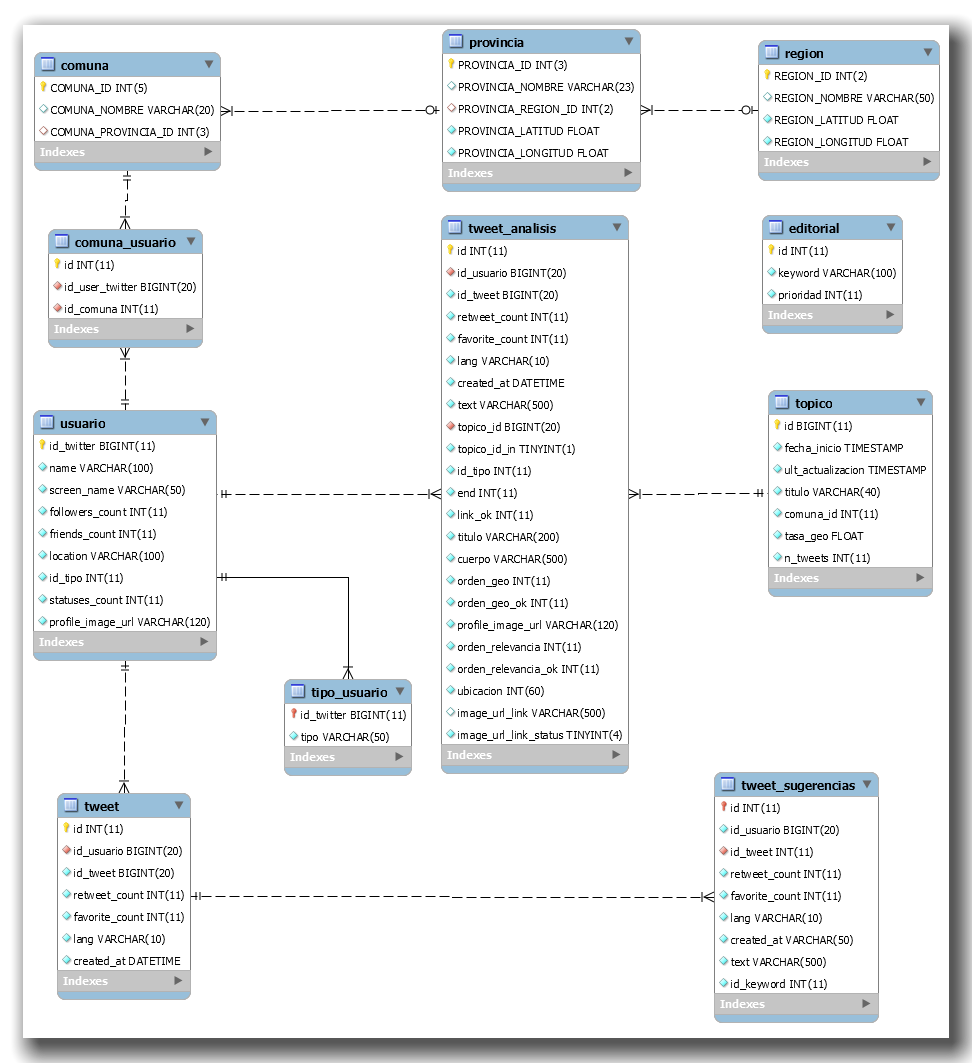
\includegraphics[width=\textwidth]{imgs/modelo_bd.png}
  \caption{Modelo de base de datos}
  \label{fig:modelo_bd}
\end{figure}


\subsection{Análisis de la línea editorial del medio objetivo}
	Para tener una directriz respecto a qué tópicos de noticias son cubiertos por el medio de prensa objetivo, se realiza un análisis de los tweets de dicho medio.
El proceso se realiza mediante el conteo de la frecuencia de las palabras contenidas en los corpus de los distintos tweets, sin considerar las palabras vacías o stopword\footnote{Stopwords o palabras vacías es el nombre que reciben las palabras sin significado como artículos, pronombres, preposiciones, etc. que son filtradas antes o después del procesamiento de datos en lenguaje natural (texto)} presentes.

\begin{algorithm}
	\caption{Obtención de las palabras más frecuentes del timeline de un conjunto de tweets}\label{ciudadesLeven}
	\begin{algorithmic}[1]
		\Function{getKeywordMedio}{tweets}
		\For{tweet in tweets}
		\For{tweet in tweets}
		\For{palabra in tweet}
		\If{stopwords.not\_in\_array(palabra)}
		\State palabras.push(palabra)
		\State frecPalabras[palabra]++
		\EndIf
		\EndFor
		\EndFor
		\EndFor
		\State return frecPalabras.ordenar()
		\EndFunction
	\end{algorithmic}
\end{algorithm}


%La cuenta de Twitter de AmorTv (\@amor\_tv) al momento de realizar la extracción con más de mil tweets de los cuales se obtuvieron los siguientes resultados:

\begin{table}[H]
	\begin{center}
		\begin{tabular}{| c | c |}
			\hline
			Posición & Palabra \\ \hline
			1 & Estudiantes \\ \hline
			2 & Valparaíso \\ \hline
			3 & Universidad \\ \hline
			4 & Toma \\ \hline
			5 & Sede \\ \hline
			6 & Represión \\ \hline
			7 & Marcha \\ \hline
			8 & Chile \\ \hline
			9 & Concepción \\ \hline
			10 & Casa Central \\ \hline
			11 & Usm  \\ \hline
			12 & Utfsm \\ \hline
			13 & Paro \\ \hline
			14 & Nacional \\ \hline
			15 & Carabineros \\ \hline
			16 & Movimiento \\ \hline
			17 & Pucv \\ \hline
			18 & Asamblea \\ \hline
			19 & Trabajadores \\ \hline
			20 & Secundarios \\ \hline
		\end{tabular}
		\caption{Tabla que muestra en orden descendente las keyword con mayor frecuencia
			en el análisis del timeline de Twitter de Amor TV}
		\label{tab:xyz}
	\end{center}
\end{table}

Se obtiene que las palabras con mayor frecuencia tienen relación con temáticas estudiantiles, manifestaciones, movimientos sociales y los lugares donde estos ocurren, que va acorde a la descripción del medio \cite{amorTV}.

%Tras el posterior análisis con los editores y miembros de amor\_tv sobre las keyword
%que con su conocimiento experto podían considerar, al momento de buscar un evento 
%noticioso agregaron las siguientes:

%	\begin{table}[h]
%	\begin{center}
%	   \begin{tabular}{| c | c |}
%		 \hline
%		   Posición & Palabra \hline
%		   1 & Trabajadores & 
%		   2 & Social & 
%		   3 & Sexismo & 
%		   4 & Santa Maria & 
%		   5 & Protesta & 
%		   6 & Movimiento & 
%		   7 & Movilización & 17 & - \\ \hline
%		   8 & Mapuche & 18 & - \\ \hline
%		   9 & Estudiantil & 19 & - \\ \hline
%		   10 & Ecológico & 20 & - \\ \hline
%		   11 & Confech  \\ \hline
%		   12 & Comunidad \\ \hline
%		   13 & Comunitario \\ \hline
%		   14 & Indígena \\ \hline
%		   15 & Autogestión \\ \hline
%		   16 Medioambiente - \\ \hline
%		\end{tabular}
%		\caption{Tabla que muestra en orden descendente las keyword con mayor frecuencia
%				en el análisis del timeline de Twitter de \@amor\_tv}
%		\label{tab:xyz}
%		 \end{center}
%	 \end{table}

%Las keyword consideradas que representan a mayor cabalidad los eventos noticiosos que
%caracterizan al medio de comunicación de prensa AmorTv, obtenidas de los análisis
%anteriores agregando variaciones de algunas palabras, son representadas gráficamente
%mediante el siguiente wordcloud:

%\begin{figure}[H]
%  \centering
%    \includegraphics[width=0.99\textwidth]{wordcloud.png}
%  \caption{WordCloud de las keyword mas representativas de los eventos noticiosos
%  característicos de AmorTv}
%  \label{fig:storyful}
%\end{figure}

\newpage

\subsection{Geolocalización de usuarios}\label{sec:geo}
\label{subsec:geo1}
	El método implementado utiliza el concepto de la distancia de Levenshtein\footnote{La distancia de Levenshtein corresponde a la cantidad de cambios necesarios en un string para transformarlo en un string objetivo.} para determinar si el texto proporcionado por el usuario como ubicación corresponde o no a una comuna existente en Chile. La información relativa a las actuales comunas, provincias y regiones de acuerdo al Decreto Exento Nº 817, del Ministerio del Interior, publicado en el Diario Oficial del 26 de Marzo de 2010 \cite{listaCodigosProvincias}. La posición GPS de cada una de las provincias se obtuvo mediante la ubicación proporcionada en \cite{dicesmapas}.

\begin{algorithm}
	\caption{Reconocimiento de ubicación del usuario mediante Levenshtein}\label{ciudadesLeven2}
	\begin{algorithmic}[1]
		\Function{getDistanciaLeven}{usuarios}
		\For{usuario in usuarios}
		\State usuario.ubicacion = limpiarPuntuacion(usuario.ubicacion)\;
		\State usuario.ubicacion = quitarNacionalidad(usuario.ubicacion)\;
		\For{comuna in comunas}
		\State dist = Levenshtein(comuna, usuario.ubicacion)\;
		\If{dist\textless MinimaDistancia}
		\State usuario.comuna = comuna\;
		\EndIf
		\EndFor
		\EndFor
		\EndFunction
	\end{algorithmic}
\end{algorithm}

%\begin{algorithm}
%	\caption{Reconocimiento de ubicación del usuario mediante SQL}\label{ciudadesSql}
%	\begin{algorithmic}[1]
%		\For{comuna in comunas}
%			\State usuariosComuna = getUsersFromBd(comuna)
%			\For{usuario in usuariosComuna}
%				\State usuario.comuna = comuna
%			\EndFor
%		\EndFor	
%	\Function{getUsersFromBd}{comuna}
%		\State sql = 'SELECT usuario WHERE usuario.ubicacion LIKE "\%" + comuna;
%		\State return execute(sql);
%	\EndFunction	
%	\end{algorithmic}
%\end{algorithm}

\subsubsection{Prueba valores distancia Levenshtein para identificar ubicación}

Para obtener cual es la distancia de Levenshtein con mejores resultados se consideró una muestra representativa de 383 usuarios elegidos de manera aleatoria y cuyo campo ubicación fuese distinto a vacío. Los resultados obtenidos fueron los siguientes:

\begin{table}[H]
	\centering
	\begin{tabular}{| c|c|c|c|}
		\hline
		D. Levenshtein & Nº match correctos & Nº match incorrectos  &  Error porcentual \\ \hline
		1   & 157 & 157 & 0,00\% \\ \hline
		2   & 172 & 164 & 2,09\% \\ \hline
		3	& 207 & 189 & 4,70\% \\ \hline
		4	& 223 & 192 & 8,09\% \\ \hline
		5	& 235 & 194 & 10,70\% \\ \hline
	\end{tabular}
	\caption {Tabla comparativa para distintas valores de distancia de Levenshtein}
\end{table}

Podemos observar que a medida que aumentamos la distancia de Levenshtein, va aumentando la cantidad de coincidencias correctas pero también la cantidad de falsas coincidencias que ocurren.

Se consideró que un error menor al 5\% es adecuado, considerando la cantidad de coincidencias correctas que aporta al conjunto. Por lo anterior se concluye que la distancia de Levenshtein a utilizar corresponde a 3. Considerando este parámetro el número de coincidencias entre el campo ubicación y los nombre estándar de las comunas es de 114.016 del total de 650.000 usuarios (correspondiente al 17,54\% de usuarios). Éste porcentaje comparativamente es mayor que el 12\% encontrado en \cite{Cheng:2010:YYT:1871437.1871535} por Cheng mediante su primera metodología explicada en  \ref{sebsec:geoestadoarte}.

Al disponer los distintos usuarios en un mapa utilizando la API de mapas de Google, se obtienen la siguiente visualización:

\begin{figure}[H]
	\centering
	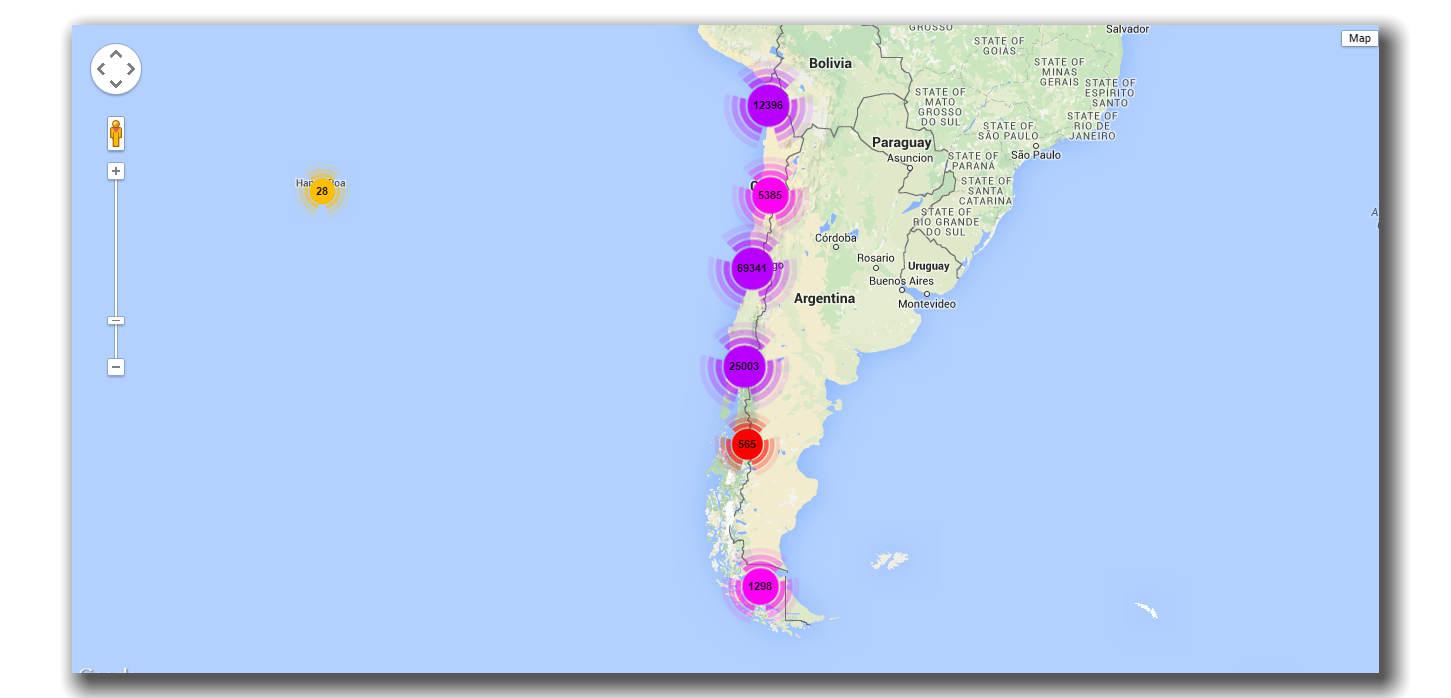
\includegraphics[width=0.9\textwidth]{imgs/mapa_usuarios.png}
	\caption{Mapa con los usuarios por ubicación geográfica}
	\label{fig:mapa_usuarios}
\end{figure}


\newpage
\subsection{Captación de usuarios}

El proceso de captación del conjunto de usuarios esta diseñado con la intención de obtener todas y todos los usuarios residentes en territorio Chileno dado que dicho catastro no existe en ninguna fuente oficial actualizada. El procedimiento se basa en las siguientes dos consideraciones: c
\begin{enumerate}
	\item Los generadores de información poseen una gran base de seguidores \cite{JavaEtAl:07}.
	\item Es habitual que los seguidores de medios de prensa al querer difundir una información le escriban un tweet a algún medio de prensa o figura de autoridad, esperando que este realice un re-tweet, para llegar también a su base de seguidores.
\end{enumerate}

El proceso de construcción de la lista de usuarios se componen de dos grandes etapas, las cuales son explicadas a continuación:

\begin{figure}[H]
	\centering
	\begin{tikzpicture}[node distance = 2cm, auto]
	
	\node [block, node distance=2.5cm, minimum width=9em, text width=8em] (i1) {\textsf{Captura de medios de prensa (MP)}};
	\node [block, below of=i1, node distance=2.5cm, minimum width=9em, text width=8em] (i2) {\textsf{Captura followers de los Medios de prensa(FMP)}};
	
	% Draw edges
	\path [line] (i1) -- (i2);
	
	\end{tikzpicture}
\caption{Diagrama conceptual con las etapas para la captación de usuarios.} \label{fig:etapas-captacion-usuarios}
\end{figure}

\subsubsection{Captura de los medios de prensa (MP)}

Para generar la lista de medios de prensa (MP) se accede a los medios de prensa registrados en las tres asociaciones más grandes de medios de comunicación de Chile:
\begin{itemize}
	\item \textit{ANP (Asociación Nacional de Prensa)} \cite{anpWebsite}: Asociación gremial constituida el 24 de agosto de 1951. Agrupa a los principales diarios y revistas del país.
	\item \textit{ANARCICH (Asociación nacional de Radios Comunitarias y Ciudadanas de Chile)} \cite{anarcichWebsite}: Es el organismo que agrupa a 300 radios comunitarias y ciudadanas de todo el país. 
	\item \textit{ARCHI (Asociación de Radiodifusores de Chile)} \cite{archiWebsite}: Fundada en 1933 es la organización gremial de medios de comunicación social más antigua de Chile.
\end{itemize}	

Ninguna de las asociaciones de medios de prensa considerados anteriormente (ANP, ANARCICH y ARCHI) cuentan con directorios públicos \cite{mediosArchi} \cite{mediosaAnp} \cite{mediosAnarcich} que provean las cuentas oficiales de twitter de los diversos medios. Por lo cual, para recolectar las cuentas de twitter de éstos, se implementa el siguiente algoritmo ejecutado por un ser humano:

\begin{algorithm}[H]
	\caption{Construcción lista de medios}\label{mediosPrensa}
	\begin{algorithmic}[1]
		\Function{getTwitterAccount}{listaMedios}
		\For{medio in listaMedios}
		\State busqueda $\gets$ 'site:twitter.com'+medio.nombre+medio.tipo +'chile'
		\State resultGoogle $\gets$ BusquedaGoogle ( busqueda, $limit=12$)
		\For{result in resultGoogle}
		\If{result.title \&\& result.description se relacionan con medio  }
		\State medio.screenName $\gets$ result.screenName
		\EndIf 
		\EndFor
		\EndFor
		\State return listaMedios
		\EndFunction	
		%	\Function{getUsersFromBd}{comuna}
		%		\State sql = 'SELECT usuario WHERE usuario.ubicacion LIKE "\%" + comuna;
		%		\State return execute(sql);
		%	\EndFunction	
	\end{algorithmic}
\end{algorithm}

Tras aplicar este algoritmo, los resultados obtenidos fueron los siguientes:

\begin{table}[H]
	\centering
	\begin{tabular}{|c|c|c|}
		\hline
		Asociación & Nº asoc. con cuentas & Nº asoc. totales \\ \hline
		ANP & 43 & 93 \\ \hline
		ANARCICH & 23 & 99 \\ \hline
		ARCHI & 9 & 304 \\ \hline
	\end{tabular}
	\caption {Cantidad de miembros de las distintas asociaciones de prensa en Chile con cuentas en Twitter al 5 de junio del 2014.}
\end{table}


\subsubsection{Captura followers de los medios de prensa (FMP)}

Tras obtener la lista de medios de prensa, mediante la API de Twitter se recopilan los seguidores de cada uno de los medios de prensa. El algoritmo continuación realiza esta tarea requiere de realizar pero debe incluir intervalos de pausas para respetar las restricciones de número de solicitudes por hora que impone la API.

\begin{algorithm}[H]
	\caption{Captura de usuarios}\label{capturaUsuarios}
	\begin{algorithmic}[1]
		\Function{GetPop}{mediosPrensa}
		\For{medio in mediosPrensa} 
		\If{GetFriendsInformation(medio, api)}
		\State Sleep(2);
		\Else
		\State Sleep(60*15);
		\State GetFriendsInformation(medio, api)
		\EndIf
		\EndFor
		\EndFunction
		
		\Function{GetFriendsInformation}{user, api}	
		\State TwitterFriends $gets$ api.GetFollowers(screenName=user)
		\If {TwitterFriends.length > 0}
		\For {Friends in TwitterFriends}:
		\State SaveInBd(Friends)
		\EndFor
		\Else
		\State Sleep(60*15);
		\EndIf
		\EndFunction
		
	\end{algorithmic}
\end{algorithm}

Una de las dificultades presentadas en el algoritmo anterior, era que ante usuarios con más de 1,5 millones de seguidores la petición a la API se demoraba un tiempo excesivo (más de 48 horas) y retornaba error por \emph{timeout} de la conexión. Para sortear esta dificultad fue necesario modificar la API Python Twitter directamente, agregando el retorno del cursor aún cuando se agota la conexión con la API y guardando los resultados parciales de las respuestas. El cursor de una llamada en la API es similar a un índice que permite realizar solicitudes de manera segmentada a la API \footnote{ Al día 26/10/2015 no se encontraba disponible la mejora en el \emph{Github} oficial de la librería \cite{pythonTwitterGithub} }. Esta modificación fue realizada en base a las recomendaciones y comentarios disponibles en los grupos de desarrolladores de la librería \cite{pythonTwitterCode} \cite{pythonTwitterGithub}. 


	\begin{algorithm}[H]
			\caption{GetFollowers}\label{getFollowers}
			\begin{algorithmic}[1]
			    \Function{GetFollowers}{self, screen\_name=None, cursor=-1}
			    \State result $\gets$ []
			    \State parameters $\gets$ \{\}
			    \While{True}: \label{getFollowers:line:line4}
				    \State next\_cursor, previous\_cursor, data $\gets$ api.GetFollowersPaged(user\_id, screen\_name, cursor)
				    \State result += [User.NewFromJsonDict(x) for x in data['users']]
				    \If{next\_cursor == 0 or next\_cursor == previous\_cursor}\label{getFollowers:line:line7}
					    \State break
				    \Else
					    \State cursor $\gets$ next\_cursor
				    \EndIf
				    \State sec $\gets$ self.GetSleepTime('/followers/list')
				    \State time.sleep(sec)
			    \EndWhile
				    \State return result
				\EndFunction				
			\end{algorithmic}
		\end{algorithm}

		\begin{algorithm}[H]
			\begin{algorithmic}[1]
				\Function{GetFollowers}{self, screen\_name=None, cursor=-1}:
					\State result $\gets$ []
					\State parameters $\gets$ \{\}
				%\If{screen\_name is not None}:
				%\State parameters['screen\_name'] $\gets$ screen\_name
				%\EndIf
				%\State parameters['include\_user\_entities'] $\gets$ True
				\color{orange}
				\State remaining $\gets$ 15
				\State ratelimited $\gets$ False
				\While{remaining $>$ 1}
					\State remaining $\gets$ remaining-1
					\State parameters['cursor'] $\gets$ cursor
					\color{black}
					\State json $\gets$ api.\_RequestUrl(url, 'GET', data=parameters)
					\State data $\gets$ api.\_ParseAndCheckTwitter(json.content)
					\If{data}
							\State result $+=$ [User.NewFromJsonDict(x) for x in data['users']]
						\If {'next\_cursor' in data}:
							\If {data['next\_cursor'] == 0 \\ OR data['next\_cursor'] == data['previous\_cursor']}
								\State break
							\Else:
								\State cursor $\gets$ data['next\_cursor']
							\EndIf
						\Else:
							\State break
						\EndIf
						\Else
						\color{orange}
							\State ratelimited $\gets$ True
							\State break
					\EndIf
					
				\EndWhile
				\State return (cursor, result, ratelimited)
				\color{black}
				\EndFunction
				
			\end{algorithmic}
			\caption{GetFollowers con mejora}\label{getFollowerModif}
		\end{algorithm}

La modificación relacionadas a la dificultad mencionada anteriormente se pueden observar en el algoritmo \ref{getFollowerModif} donde fueron resaltadas con otro color. Principalmente incorpora un límite de llamadas a la API a 15 llamadas consecutivas de tal manera de reducir el intervalo de respuesta de la llamada, este parámetro fue determinado en base a la restricción de la API de Twitter. Esta modificación permite ir guardando nuevos datos de manera frecuente sin necesidad de esperar hasta completar todos los followers de un usuario. En  la función original las líneas ~\ref{getFollowers:line:line4} y ~\ref{getFollowers:line:line7} mantienen el ciclo de consultas por followers hasta que los cursores indican que no existen más followers por recibir (y sólo cumplida esa condición retorna datos).

El algoritmo se demora en promedio 2,6945531 segundos en descargar los datos de un usuario y almacenarlos en el sistema.

\subsection{Captura de tweets}

El proceso de captura de tweets se realiza obteniendo los 100 últimos tweets de cada uno de los usuarios y usuarias recolectadas en la fase anterior, sin discriminación ni priorización alguna, tal como muestra el siguiente algoritmo:

\begin{algorithm}[H]
	\caption{Algoritmo para la captura de tweets.}\label{getTweets}
	\begin{algorithmic}[1]
		\Function{GetTweets}{}
		\State usuarios $\gets$ getUsersFromBD();
		\For {usuario in usuarios}
		\State GetUserTimeline(id\_user=usuario.id);
		\EndFor
		\State time.sleep(5);
		\EndFunction
		
		\Function{GetUserTimeline}{id\_user}:
		\State statuses $\gets$ api.GetUserTimeline(user\_id=id\_user,count=100);
		\State SaveTweetInBD(statuses);
		
		\If {statuses.error == 34}
		\Comment{La cuenta ya no existe}
		\State return 1;
		\EndIf
		
		\If {statuses.error == 179}
		\Comment{La cuenta es privada}
		\State return 1;
		\EndIf
		
		\If {statuses.error == 88}
		\Comment{Limite de solicitudes excedidas}
		\State time.sleep(5*60);
		\State return
		\EndIf
		\EndFunction
	\end{algorithmic}
\end{algorithm}

El algoritmo planteado principalmente en su primera etapa realiza una búsqueda de los usuarios y sus respectivos estados referentes a si han sido recolectados sus últimos tweets (en cuyo caso se van a buscar los 100 tweets más recientes a partir del último recogido) o no (en cuyo caso se van a buscar los 100 tweets más recientes), posteriormente se almacenan en la base de datos los tweets recibidos. Es importante resaltar que este algoritmo gestiona las distintas pausas necesarias para respetar los límites de la API Twitter y posibles restricciones sobre si la cuenta no existe o es privada. 

El algoritmo se demora en promedio 0,9658139 segundos en descargar los tweets de un usuario y almacenarlos en el sistema.

\subsection{Procesamiento de los tweets}

El procesamiento de los tweets se define en tres procesos:
\begin{enumerate}
	\item{Definición del tópico.}
	\item{Obtención del conjunto de tweets relacionados al tópico.}
	\item{Depuración de conjunto de tweets relacionados al tópico.}
\end{enumerate}

\subsubsection{Definición del tópico}

Un tópico son las palabras claves que definen una búsqueda temática realizada por el administrador del sistema mediante la plataforma web, cada tópico posee los siguientes atributos:
\begin{itemize}
	\item \textit{Fecha de inicio} : Se refiere a la fecha de inicio de emisión de los tweets objetivos que se requiere reunir.
	\item \textit{Fecha última actualización}: Se refiere a la última fecha en la cual se realizó alguna modificación referente al tópico.
	\item \textit{Título}: Se refiere a las palabras claves que definen al tópico. 
	\item \textit{Comuna}: Comuna relacionada al tópico.
	\item \textit{Tasa de contenidos georeferenciados}: Relación entre tweets con relación geográfica y los tweets totales.
	\item \textit{Cantidad de tweets relacionados}: Total de tweets depurados del conjunto de tweets relacionados. 
\end{itemize}

\subsubsection{Obtención del conjunto de tweets relacionados al tópico}

Para obtener el conjunto de tweets relacionados al tópico se realiza una búsqueda en todos los tweets emitidos durante el periodo de interés
y que contengan las palabras claves que definen al tópico. Posteriormente se eliminan los tweets que poseen una similitud 0.85\% en sus textos 
utilizando la librería \emph{difflib}. Esta consulta se demora entre 30 y 130 segundos.

\begin{algorithm}[H]
	\caption{Obtención del conjunto de tweets relacionados al tópico}\label{getTweetsKeyword}
	\begin{algorithmic}[1]
		
		\Function{getTweetKeyword}{keywords,fecha}:
		%\Comment{Query tematica: va a buscar tweets que contengan una cierta keyword y retorna un array con las palabras que la contengan}
		\State tweets $\gets$ getTweetsFromBD(keywords, fecha);
		\State tweets $\gets$ eliminacionTweetsRepetidos(tweets);
		\State return tweets
		\EndFunction
	\end{algorithmic}
\end{algorithm}	



\subsubsection{Depuración de conjunto de tweets relacionados al tópico}

El proceso de depuración del conjunto de tweets obtenidos en el proceso anterior considera dos etapas distintas dependiendo del volumen de los tweets involucrados.

Un gran desafío en la depuración de los tweets, es discernir si un tweet en particular se relaciona o no con la temática del tópico, o por el contrario, si responde a una temática completamente distinta (y fue relacionado con el tópico únicamente por concordancia textual). Por ejemplo, si el tópico se refiere a "la paralización del registro civil", con la keyword 'paro' se busca excluir todos los tweets que se refieran a un "paro cardíaco" o de "la acción de levantarse".

Para aplicar un filtro efectivo se consideran las siguientes premisas:
\begin{itemize}
	\item El administrador del sistema posee poco tiempo (una tarea como eliminar filtros es un trabajo repetitivo y monótono, que requiere varias horas hombres para su desarrollo).
	\item Es fundamental filtrar con precisión los tweets que no corresponden a la temática.
\end{itemize}

Para conjuntos de tweets de menos de 300 tweets se considera que su depuración puede ser realizada de manera manual, debido a que no es un gran conjunto de datos y su análisis manual no demanda tiempo excesivo.

Para conjuntos de 300 tweets o más se considera que su depuración manual es muy extensa y debe ser automatizada. Para su automatización se implementa un clasificador de Bayes-Naive. El clasificador Bayer-Naive utilizado es una implementación de la librería Python Textblob \cite{textblobWebsite}.

Los tamaños de los distintos conjuntos dependiendo del tamaño del conjunto de tweets es el siguiente:

\begin{table}[h]
	\centering
	\begin{tabular}{| c | c | c |}
		\hline
		Nº tweets & Nº Entrenamiento & Nº Validación \\ \hline
		N $\leqslant$ 300	& Manual & Manual \\ \hline
		0 $\leqslant$ N $\leqslant$ 430	& N $*$ 0,2 & N*0,3	\\ \hline
		430 $\leqslant$ N & 200 & 100	\\ \hline
	\end{tabular}
	\caption {Cantidades conjuntos del clasificador utilizado}
\end{table}

Estas cantidades fueron determinadas de manera empírica en base a recomendaciones recogidas en foros y experimentos propios realizados con la librería de tal manera de obtener una precisión de clasificación siempre superior a 85\%.

\begin{algorithm}
	\caption{Clasificador Bayes-Naive para determinar si es miembro o no del tópico.}\label{CrearClasificador}
	\begin{algorithmic}[1]
		\Function{crearClasificador}{}
		\State restoTweets, tweetsValidacion, tweetsEntrenamiento $\gets$ SepararConjuntos(tweets);
		\State clasificador.entrenar(tweetsEntrenamiento)
		\State clasificador.validar(tweetsValidacion)
		
		\For {tweet in restoTweets}
			 \State clasificador.clasificar(tweet);
		\EndFor
		\EndFunction
	\end{algorithmic}
\end{algorithm}

	

La clasificación de los distintos tweets en las categorías \emph{pertenece al tópico} y \emph{no pertenece al tópico} se realiza mediante la función \emph{prob\_classify(tweet).max()} que retorna la etiqueta de la clasificación que posee mayor probabilidad según el clasificador para el tweet en específico \cite{naivebayesdoc}.

\subsubsection{Orden geográfico}

El orden geográfico dota al prototipo de un filtro que privilegia a las fuentes cercanas al lugar indicado como origen del hecho noticioso en desmedro de aquellas que se ubican a mayor distancia geográfica.

El orden geográfico se basa en la posición geográfica del autor de cada tweet analizado  en la sección ~\ref{subsec:geo1}. Inicialmente se obtienen las comunas con menor distancia a la comuna central determinada como origen del tópico y se aumenta progresivamente la distancia hasta clasificar todos los tweets de autores geoposicionados, los tweets sin ubicación son desplazados al final del ranking. 

\begin{algorithm}[H]
	\caption{Orden Geográfico}\label{OrdenGeo}
	\begin{algorithmic}[H]
		\Function{ordenGeografico}{comunaCentral}
		\State d $\gets$ 0
		\State i $\gets$ 0
		\State tweets $\gets$ getTweetsUbicados()
		\While{todosAsignados(tweets) == false}
			\State comunas $\gets$ getComunasFromDistance(d, comunaCentral)
			\For{comuna in comunas}
				\State tweets $\gets$ getTweetsFromComuna(comuna)
				\For{ tweet in tweets}
					 \State tweet.ordenGeo $\gets$ i
					 \State i $\gets$ i + 1
				\EndFor
			\EndFor
			\State d $\gets$ d + 1
		\EndWhile
		\EndFunction	
	\end{algorithmic}
\end{algorithm}


\subsubsection{Orden de relevancia}\label{subsubsec:orden-rel} 	

El objetivo de este \emph{ranking}, es generar un mecanismo que ordene los contenidos en base a su relevancia, entendida como el grado de utilidad de un tweet para informar al usuario respecto al evento en cuestión.

Para su diseño se considera la cantidad de re-tweets con que cuenta el tweet basado en el razonamiento abordado en \cite{conf/cikm/UysalC11} donde se considera que la acción de re-tweet resumen en un solo indicador, la importancia que le atribuyen sus lectores al contenido del tweet y lo replican, porque lo consideran relevante y en el estudio de la intención realizado en \cite{Yamaguchi:2010:TTU:1991336.1991364} referente a que si la intención del re-tweet es difundir (intención buscada por el prototipo, tweets que busquen informar y difundir sobre el tópico), es bastante probable que posea una gran cantidad de re-tweet, no así los tweets conversacionales .
 
 En el diseño también se considera la fecha de emisión del tweet, implementando un sistema de tres clasificaciones basado en el ranking desarrollado en \cite{Dong:2010:TEI:1772690.1772725} con la diferencia que se utilizan tres grados de clasificación y no cinco.

El mecanismo de descenso implementado considera que un tweet esta \emph{fuera de la fecha} cuando la fecha de emisión del tweet es 4 días antes que la fecha de emisión del tweet más reciente del conjunto de tweets y considera que un tweet esta totalmente \emph{fuera de fecha} cuando la fecha de emisión del tweet es 10 o más días antes que la fecha de emisión del tweet más reciente del conjunto. Para los tweets \emph{fuera de fecha} se aplica un descenso de una categoría, mientras que para los tweets \emph{totalmente fuera de fecha} se aplica un descenso de dos categorías.

\begin{algorithm}[H]
	\caption{Orden Relevancia}\label{OrdenRel}
	\begin{algorithmic}[1]
		\Function{ordenRelevancia}{}
		\State maxRT $\gets$ getMaxRT()
		\State minRT $\gets$ getMinRT()
		\State fechaMasReciente $gets$ getFechaMasReciente()
		\State firstClass, secondClass, thirdClass $gets$ dividirConjuntoPorRT(tweets)
		
		\For{ tweet in firstClass}
		\State deltaFecha $\gets$ diff(fechaMasReciente, tweet.fecha)
		
		\If{ deltaFecha $\geqslant$ 4 dias}
			\State tweet.clase $\gets$ tweet.clase - 1
			\ElsIf { deltaFecha $\geqslant$ 10 dias}
				\State tweet.clase $\gets$ tweet.clase - 2
		\EndIf
		
		\EndFor
		
		\For{ tweet in secondClass}
		\State deltaFecha $\gets$ diff(fechaMasReciente, tweet.fecha)
			\If{ deltaFecha $\geqslant$ 4 dias}
				\State tweet.clase $\gets$ tweet.clase - 1
			\EndIf
		\EndFor	
		\EndFunction
	\end{algorithmic}
\end{algorithm}

%\emph{Resultados}
	
%	Para realizar experimentos con este orden se seleccionaron X tweets de forma aleatoria de un topico determinado, estos tweets fueron presentados de forma aleatoria en un formulario de papel en donde por cada tweet se presentaba:
	
%	\begin{itemize}
%		\item Texto del tweet
%		\item Fecha del tweet
%	\end{itemize}
	
%	Las instrucciones del formulario para cada evaluador experto indicaba: \emph{Ordene los siguientes textos de tweets, colocando un numero en la linea ubicada a la derecha de cada texto, según su relevancia (grado de utilidad del tweet para informar al usuario respecto al evento en cuestión) }. Los resultados obtenidos fueron los siguientes:
	
%	\input{result-orden-rel.tex}
		

\subsubsection{Panel de enlaces}

Esta vista fue desarrollada con la intención de crear una sección de \emph{bibliografía multimedia} de un tópico. Mediante un algoritmo que recoge todos los enlaces compartidos mediante los tweets del tópico y los presenta a modo
de grilla.

Esta vista permite en mismo espacio, acceder a enlaces externos que permiten extender la información del tópico aportada por los distintos tweets, así como acceder a enlaces de distintas posturas permitiendo entre otras cosas contraponer la forma en que presentan la información, profundidad, etc.

Los enlaces son ordenados en base a su tweet de origen, del más reciente al menos reciente y luego del que posee más re-tweets al que posee menos.

\begin{algorithm}
	\caption{Obtención de enlaces externos contenidos en los tweets}\label{getURLAlgo}
	\begin{algorithmic}[H]
		\Function{GetUrlsByTweets}{tweets}
		tweets $\gets$ ordenarRelevancia(tweets);
		%\State Obtener lista de tweets del topico ordenados del más reciente al menos reciente, del que posee más re-tweets al que posee menos
		\For{ tweet in tweets}
			\If{hasURL(tweet)}
				\State urls.append(tweet.url)
			\EndIf
		\EndFor
		\For{url in urls}
			\State url.titulo, url.link, url.imagen $\gets$ getInformationURL(url)
		\EndFor 
		\EndFunction

	\end{algorithmic}
\end{algorithm}

Debido a la gran versatilidad del origen que poseen los distintos enlaces compartidos, existen dificultades en su recolección por distintos motivos como: URL incorrectas o inexistentes, textos que no es posible manipular, etc.

Para capturar los datos del enlace, se utilizó la librería lxml \ref{itm:lxml} de Python, navegando por la estructura del documento HTML se extrae el título, en enlace completo y una imagen representativa. Las condiciones mínimas que se aplica a cada uno de estos datos, es que el titulo tenga más de 10 caracteres, que la imagen posea el metatag \emph{image} de Opengraph \cite{openGraphProtocol} y que el enlace no retorne error 404 (página no encontrada).


	
	   

\subsubsection{ON/OFF Medios de prensa}
El botón \emph{ON/OFF Medios de prensa} permite ocultar o mostrar todos los tweets de la lista que hayan sido emitido por una cuenta registrada en el sistema como medio de prensa. Esta funcionalidad fue desarrollada con la intención de contar con la opción voluntaria de visualizar o no, los tweets de las cadenas de prensas, para privilegiar la lectura de tweets generados por personas o entidades sociales.

	
	\chapter{Evaluación y discusión}\label{chap:discusion}
	\section{Vistas del prototipo}	
\begin{itemize}
	\item {Vista nueva búsqueda tópico}: Esta vista presenta una barra de búsqueda para ingresar las palabras claves del tópico, la fecha inicial del tópico y un select box para la ubicación del suceso. 
	\begin{figure}[H]
		\centering
		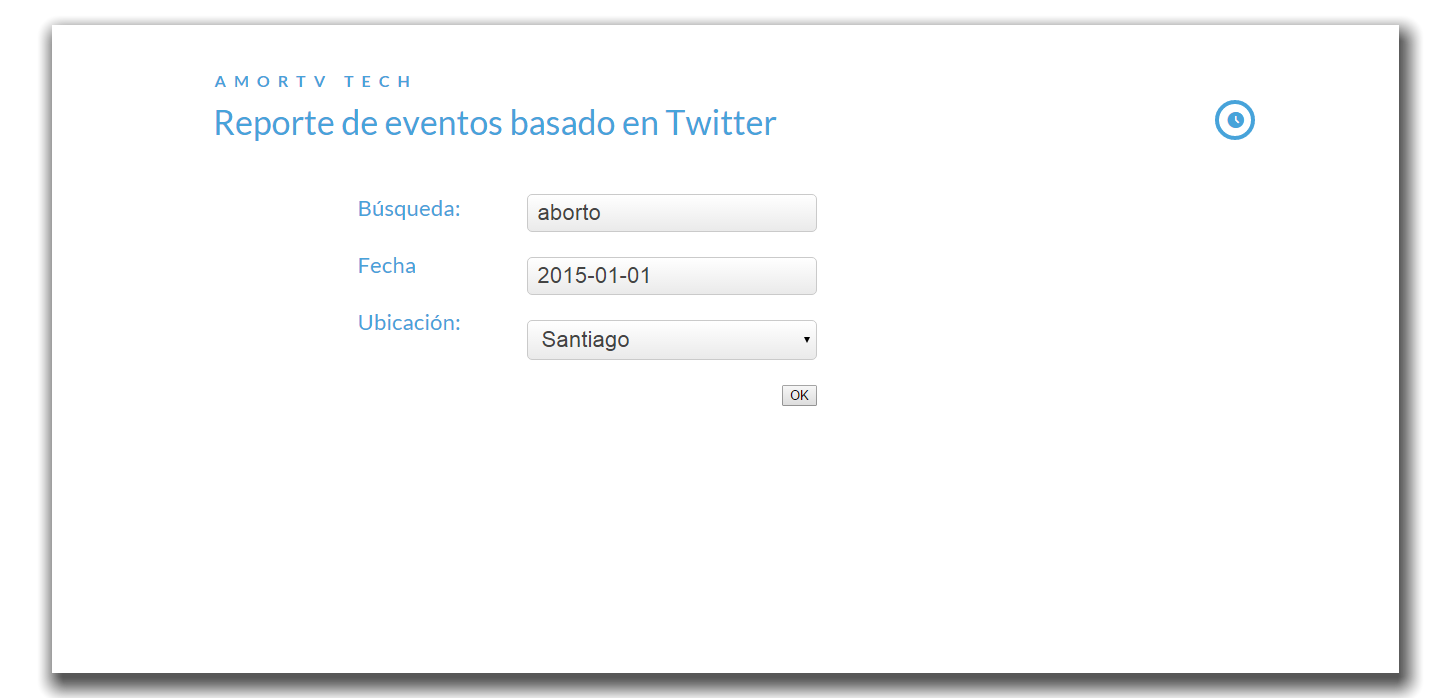
\includegraphics[width=0.9\textwidth]{imgs/vistas_newsearch.PNG}
		\caption{Vista nueva búsqueda tópico}
		\label{fig:vista_newsearch}
	\end{figure}
	
	\item {Vista resultados tweets para nuevo tópico}: Esta vista incluye la cantidad de tweets relacionados al tópico que contabilizó el algoritmo.
	\begin{figure}[H]
		\centering
		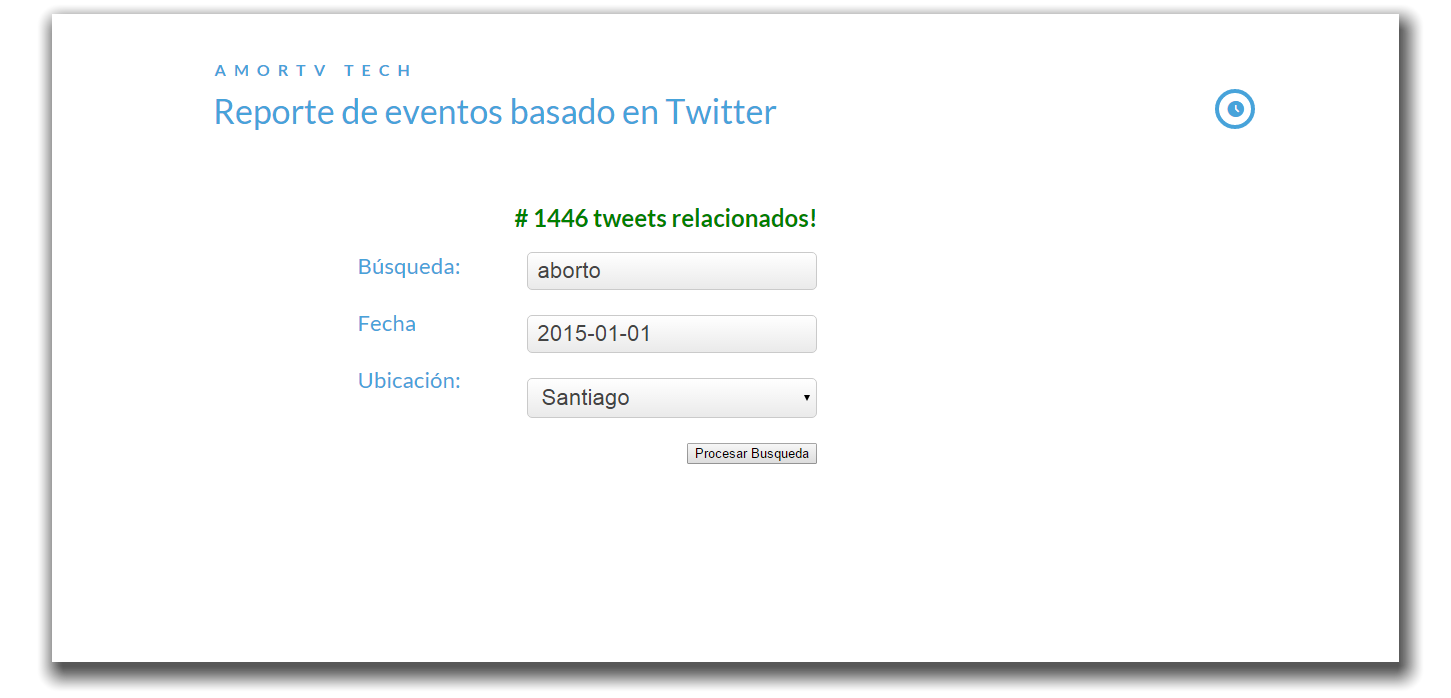
\includegraphics[width=0.9\textwidth]{imgs/vistas_newsearch_results.PNG}
		\caption{Vista resultados tweets para nuevo tópico}
		\label{fig:vista_newsearch_resultados}
	\end{figure}
	\newpage
		\item {Vista tópicos}: Esta vista presenta la lista de los tópicos que han sido buscados previamente, en cada tópico se indica distintas características del tópico: cantidad de tweets, fecha de inicio y ubicación.
		\begin{figure}[H]
			\centering
			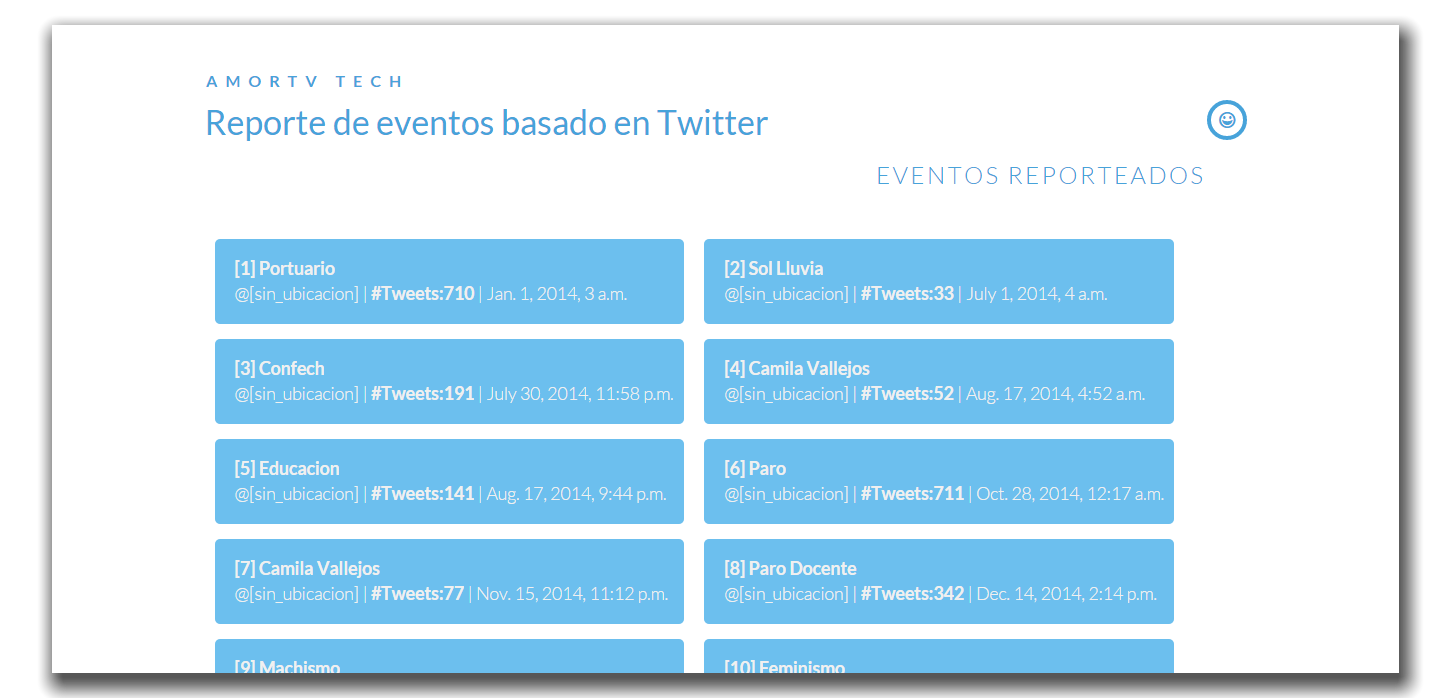
\includegraphics[width=0.9\textwidth]{imgs/vistas_topicos.PNG}
			\caption{Vista de tópicos}
			\label{fig:vista_topicos}
		\end{figure}
	
	\item {Vista orden geográfica}: Esta vista presenta un listado de los tweets relacionados en orden geográfico, en la parte superior de la lista están los tweets emitidos en la ubicación del tópico mientras que en la parte inferior de la lista están los tweets emitidos en la comuna más distante físicamente de la ubicación del tópico.
	\begin{figure}[H]
		\centering
		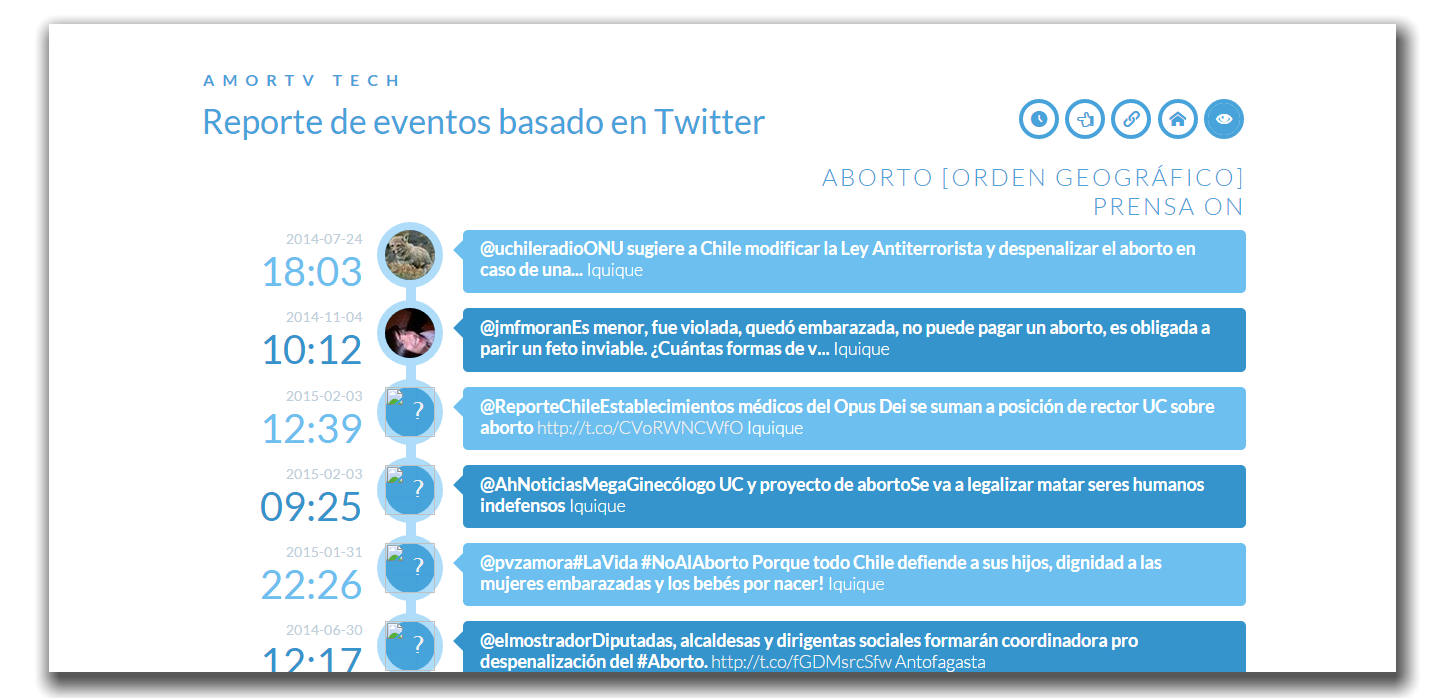
\includegraphics[width=0.9\textwidth]{imgs/vistas_geo.PNG}
		\caption{Vista de orden geográfico}
		\label{fig:vista_geo}
	\end{figure}
	
	\item {Vista orden por relevancia}: Esta vista presenta un listado de los tweets relacionados en orden descendiente por relevancia.
	\begin{figure}[H]
		\centering
		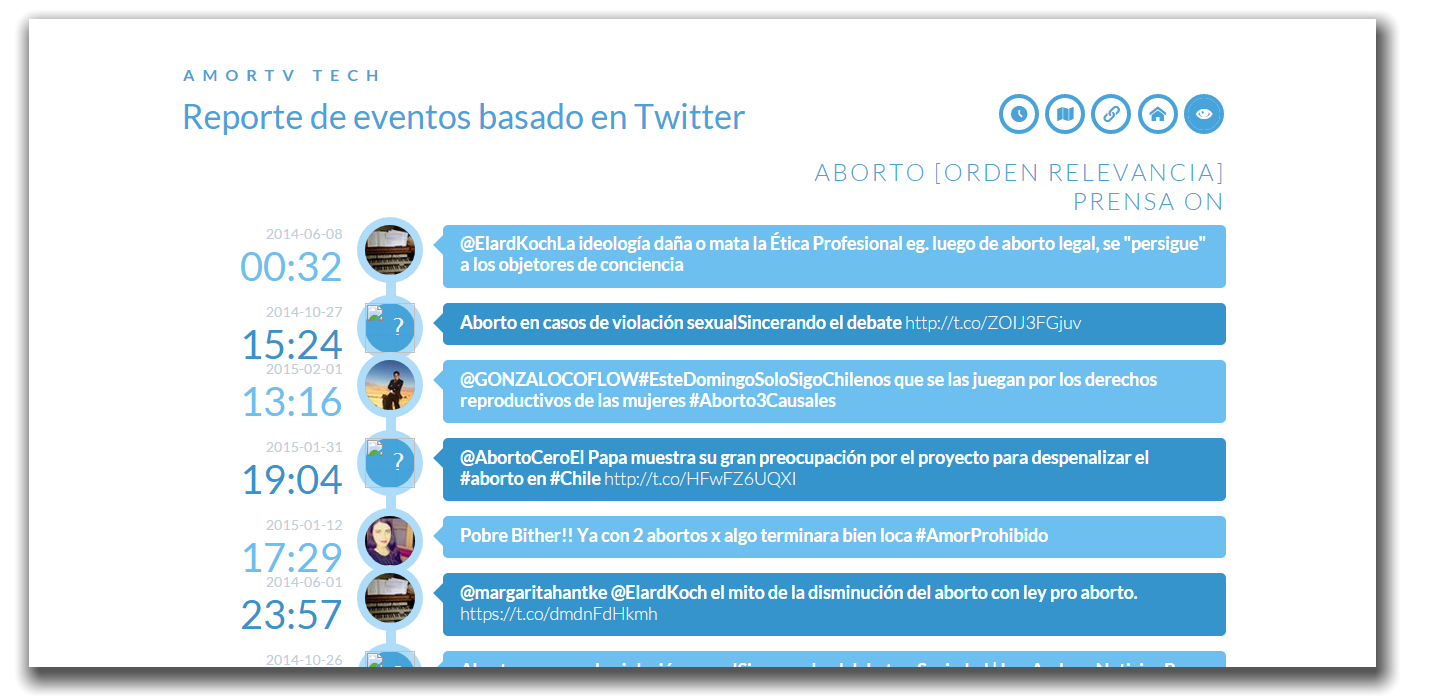
\includegraphics[width=0.9\textwidth]{imgs/vistas_rel.PNG}
		\caption{Vista de orden por relevancia}
		\label{fig:vista_rel}
	\end{figure}
		
	\item {Vista orden temporal}: Esta vista presenta un listado de los tweets relacionados en orden descendiente de fecha de emisión.
	\begin{figure}[H]
		\centering
		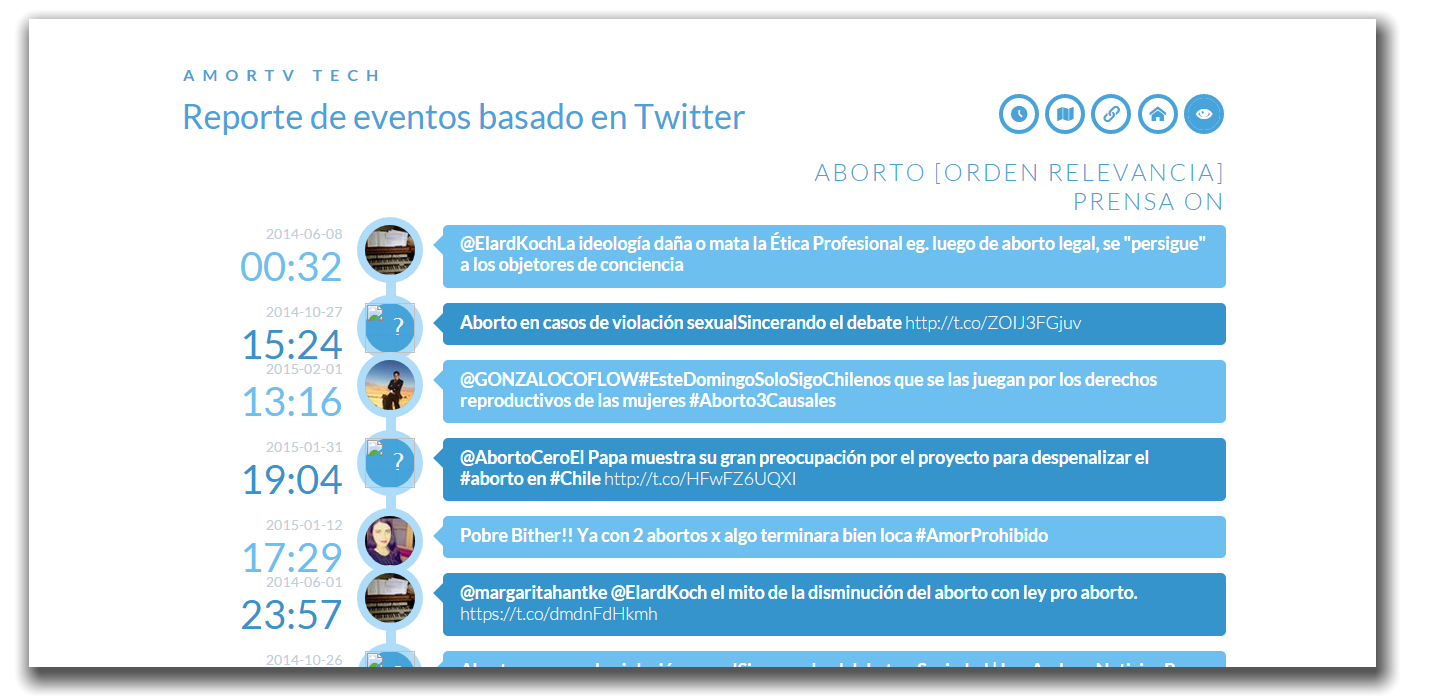
\includegraphics[width=0.9\textwidth]{imgs/vistas_rel.PNG}
		\caption{Vista de orden temporal}
		\label{fig:vista_temp}
	\end{figure}
	
	\item {Vista links}: Esta vista presenta un listado de los enlaces externos contenidos en los distintos tweets relacionados con el tópico, cada una de las casillas presenta una imagen previa del contenido y el titulo del contenido del enlace. Las casillas blancas mostradas en la imagen corresponden a que la imagen previa no pudo ser obtenida.
	\begin{figure}[H]
		\centering
		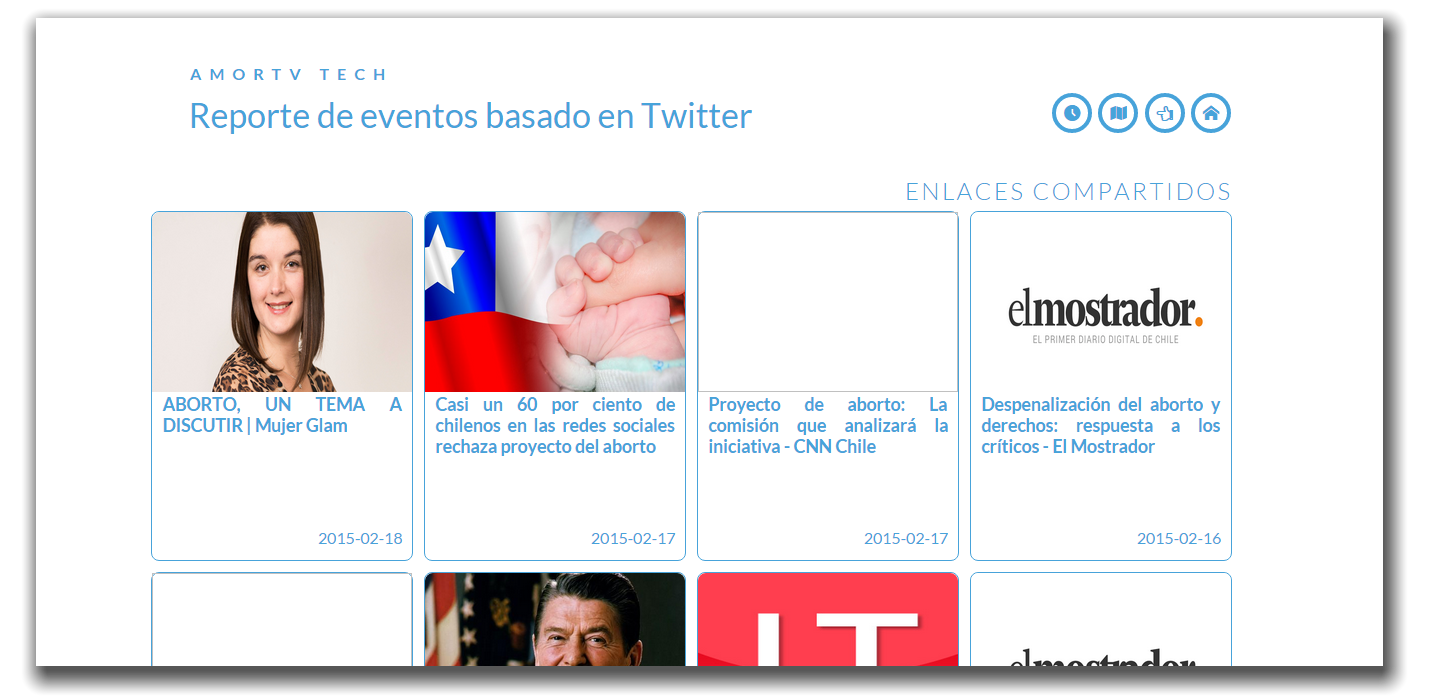
\includegraphics[width=0.9\textwidth]{imgs/vistas_links.PNG}
		\caption{Vista de links}
		\label{fig:vista_links}
	\end{figure}
		
	\item {Botón ON/OFF Prensa}: Este botón oculta o muestra los tweets emitidos por las cuentas identificadas como medio de prensa.
	\begin{figure}[H]
		\centering
		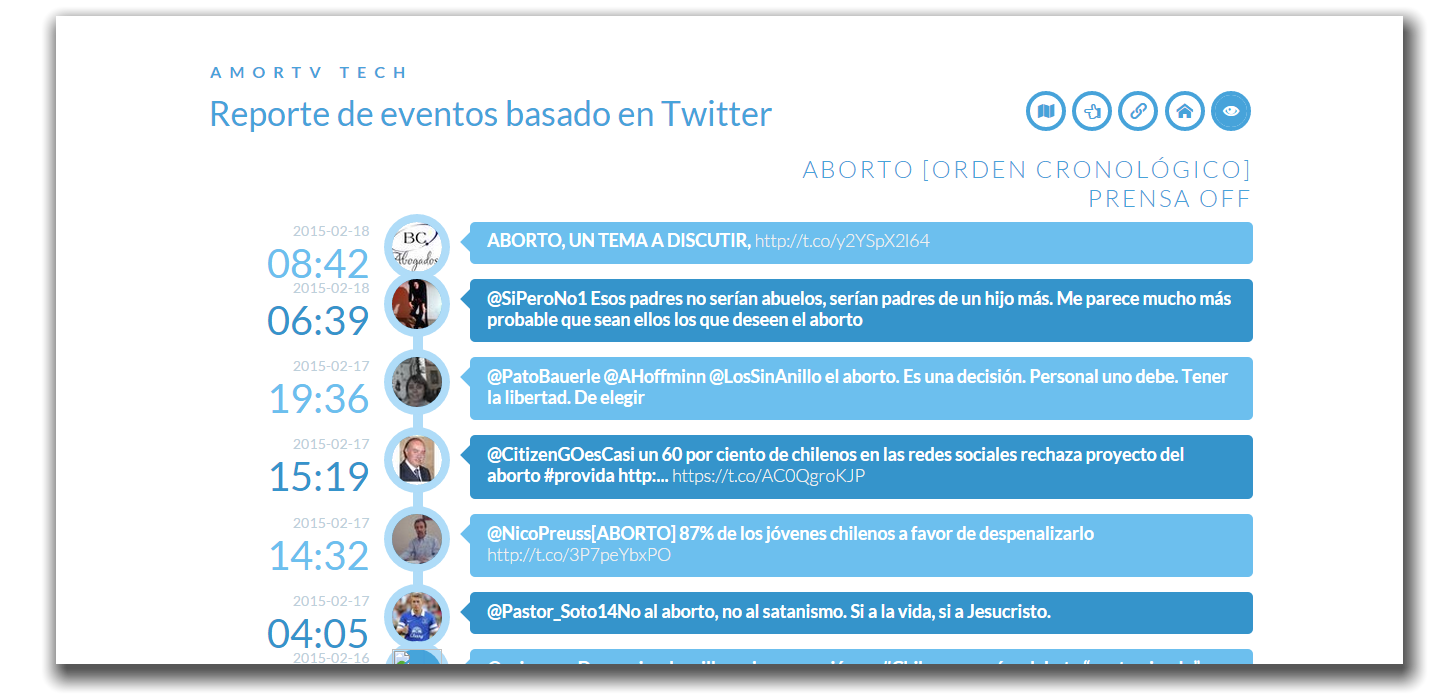
\includegraphics[width=0.9\textwidth]{imgs/vistas_prensa_off.PNG}
		\caption{Vista de tópicos}
		\label{fig:vista_btnprensa_off}
	\end{figure}
	

	
\end{itemize}
		
\section{Caracterización de la población de datos capturados}
En la siguiente sección se presenta una caracterización general de los datos capturados hasta el cierre de esta memoria con intenciones de aportar a los datos estadísticos relativos a Twitter en territorio Chileno.

Las cantidades de datos capturados son los siguientes:

\begin{table}[H]
	\centering
	\begin{tabular}{| l | c |}
		\hline
		Tipo de dato    & Nº\\ \hline
		Usuarios    & 650.000 \\ \hline
		Tweets		& 17.300.000 \\ \hline
	\end{tabular}
	\caption {Cantidad de datos capturados}
\end{table}

Características referentes a Twitter 

\begin{figure}[H]
	\centering
	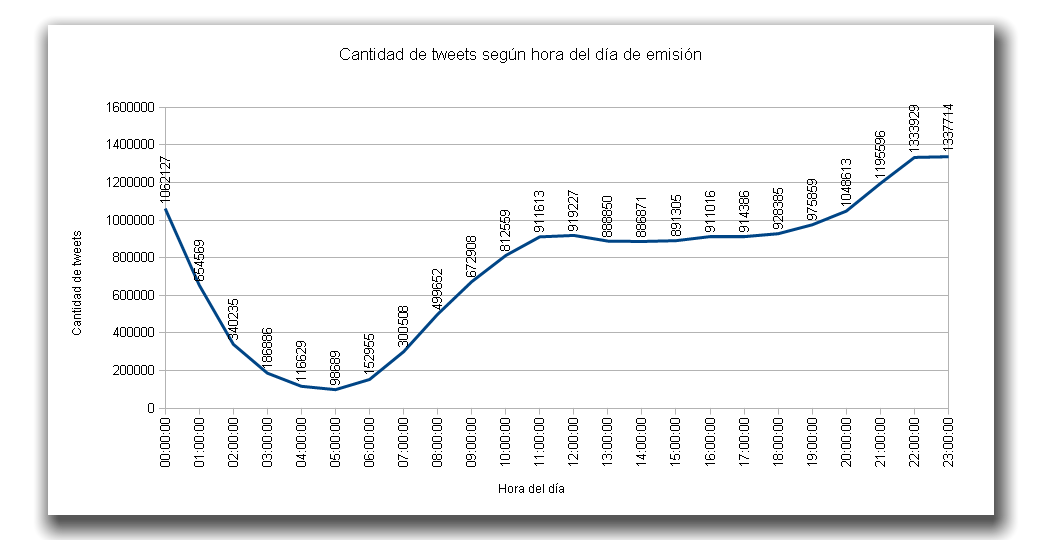
\includegraphics[width=1\textwidth]{imgs/tweets_por_hora_del_dia.png}
	\caption{Distribución de tweets por hora de emisión}
	\label{fig:tweets_por_hora}
\end{figure}

En la figura \ref{fig:tweets_por_hora} se grafica la distribución horaria de la emisión de los tweets captados. Se puede observar que las horas donde se emiten mayor cantidad de tweets comprende el periodo del día que va desde las 20:00 hrs. hasta las 23:00 hrs. mientras que el de menor emisión de tweets comprenden el periodo de horas desde las 3:00 hrs. hasta las 6:00 hrs. Se observa además que existe un periodo relativamente constante en emisión de tweets que se desarrolla desde las 11:00hrs. hasta las 20:00hrs.

La figura \ref{fig:tweets_porcentual_por_hora_por_region} representa la actividad porcentual por horas separado por región, donde se observa que existe un comportamiento similar al descrito anteriormente.

\begin{figure}[H]
	\centering
	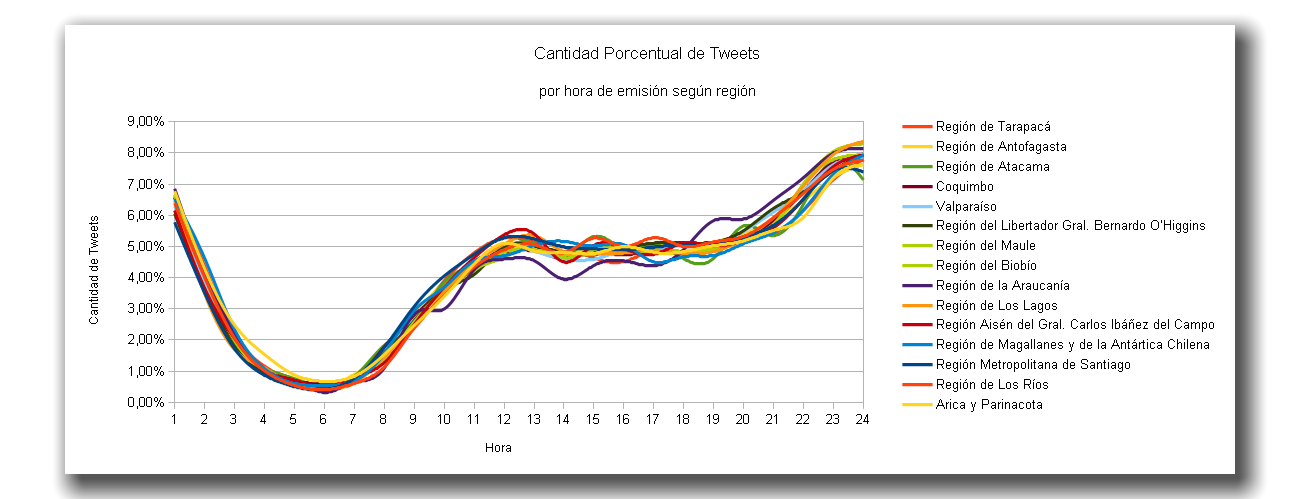
\includegraphics[width=1\textwidth]{imgs/cantidad_porcentual_de_tweets_por_hora_y_regiones.png}
	\caption{Distribución porcentual de tweets por hora de emisión según región}
	\label{fig:tweets_porcentual_por_hora_por_region}
\end{figure}



\textbf{Cantidad de re-tweets por usuario} \\

\begin{table}[H]
	\centering
	\begin{tabular}{| l | c |}
		\hline
		Medida   & Nº\\ \hline 
		Moda    & 0 \\ \hline
		Rango    & 3.424.962 \\ \hline
		Desviación Estándar    & 26.900,05 \\ \hline
		Promedio   & 711,31 \\ \hline
	\end{tabular}
	\caption {Datos cuantitativos respecto a los RT}
	\label{resumen_rt}
\end{table}

La tabla \ref{resumen_rt} nos permite observar que en cuanto al parámetro de RT el conjunto de tweets existe una variabilidad increíble respecto al promedio, lo que sugiere que existen tweets particulares con cantidades extremas de re-tweets. Tras analizar con más detalles los tweets con mayores cantidades de re-tweets se identifica una hecho insólito incluso para las macrocifras de Twitter: el tweet con más re-tweets corresponde a la famosa \emph{selfie} tomada por Ellen DeGeneres en los Oscar 2014 en conjunto a varias estrellas del cine que alcanzó el record en re-tweets con la suma de 2,5 millones de re-tweets.

\begin{figure}[H]
	\centering
	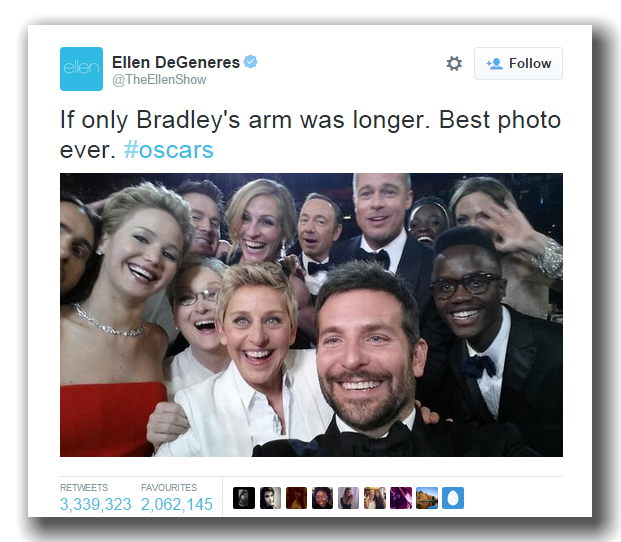
\includegraphics[width=0.5\textwidth]{imgs/ellen_selfie.png}
	\caption{Tweet que generó nuevo record del mensaje más re-tweeteado.}
	\label{fig:ellen_selfie}
\end{figure}

\textbf{Cantidad de favoritos por usuario} \\

\begin{table}[H]
	\centering
	\begin{tabular}{| l | c |}
		\hline
		Medida   				& Nº\\ \hline 
		Moda    				& 0 \\ \hline
		Rango    				& 18423 \\ \hline
		Desviación Estándar    	& 16,28 \\ \hline
		Promedio   				& 0,2602 \\ \hline
	\end{tabular}
	\caption {Datos cuantitativos respecto a los FAV}
\end{table}

De manera similar al caso de los re-tweets, la cantidad de favoritos presenta una desviación estándar más grande que el promedio captado, con la diferencia que el rango es menor. En comparativa con la tabla anterior es posible apreciar una diferencia de al menos tres ordenes de magnitud entre las medias de ambos cuantificadores.\\

\textbf{Cantidad de tweets por usuario} \\

Respecto a la cantidad de tweets se observa que el promedio son 627 tweets por cuenta de usuario como se observa en la siguiente tabla: 

\begin{table}[H]
	\centering
	\begin{tabular}{| l | c |}
		\hline
		Medida   				& Nº\\ \hline 
		Moda    				& 0 \\ \hline
		Rango    				& 718.249 \\ \hline
		Desviación Estándar    	& 4.700,45\\ \hline
		Promedio   				& 627,5728 \\ \hline
	\end{tabular}
	\caption {Cantidad de tweets por usuario}
	\label{resumen_tweets}
\end{table}
\textbf{Cantidad de Seguidores por usuario} \\

\begin{table}[H]
	\centering
	\begin{tabular}{| l | c |}
		\hline
		Medida   				& Nº\\ \hline 
		Moda    				&  1 \\ \hline
		Rango    				& 5.372.178\\ \hline
		Desviación Estándar    	& 16.504,96 \\ \hline
		Promedio   				& 427,64 \\ \hline
	\end{tabular}
	\caption {Cantidad de seguidores por usuario}
	\label{table:followers_por_usuario}
\end{table}

\textbf{Cantidad de Amigos por usuario} \\

\begin{table}[H]
	\centering
	\begin{tabular}{| l | c |}
		\hline
		Medida   				& Nº\\ \hline 
		Moda    				& 40\\ \hline
		Rango    				& 1.393.022\\ \hline
		Desviación Estándar    	& 5.283,16 \\ \hline
		Promedio   				& 364,50\\ \hline
	\end{tabular}
	\caption {Cantidad de amigos por usuario}
	\label{table:friends_por_usuario}
\end{table}

Tras comparar las tablas \ref{table:followers_por_usuario} y la tabla \ref{table:friends_por_usuario} se observa que existe una diferencia muy ajustada en los promedios obtenidos, pero que el valor máximo es superior en el caso de la cantidad de seguidores que en la cantidad de amigos de los usuarios. 

Utilizando las clasificaciones para usuarios realizadas en \cite{conf/cikm/UysalC11} en Chile su distribución es la siguiente:

\begin{table}[H]
	\centering
	\begin{tabular}{| l | c |}
		\hline
		Nombre Categoría  		& Nº\\ \hline 
		Élite Global   			& 784 \\ \hline 
		Élite Local   				& 1.611\\ \hline
		Usuario Corriente			& 624.564\\ \hline
	\end{tabular}
	\caption {Cantidad de usuarios según clasificación realizada en \cite{conf/cikm/UysalC11}}
	\label{table:cantidad_usuarios_por_clasificacion}
\end{table}

Cómo dato adicional a la tabla \ref{table:cantidad_usuarios_por_clasificacion} existen 37.808 que teniendo menos de 1000 followers no cumplen con el criterio de tener menos de 1000 amigos.\\

\textbf{Posicionamiento geográfico de los usuarios}\\

Respecto al posicionamiento de los usuarios con el método revisado en \ref{sec:geo} se obtuvo la siguiente distribución por regiones:

%revisar pagina 20 seccion 4.2.5

\begin{table}[H]
	\centering
	\begin{tabular}{| p{5.5cm} | c | c | c | c |}
		\hline
			\multirow{2}{*}{Región} & \multicolumn{2}{c|}{Usuarios Twitter} & \multicolumn{2}{c|}{Población real} \\ \cline{2-5}
			& Usuarios (M) & Porcentaje & Personas (M) & Porcentaje \\ \hline
			Región de Arica y Parinacota & 1,914 & 1,68 & 185,0 & 1,1 \\ \hline 
			Región de Tarapacá & 4,477 & 3,93 & 314,5 & 1,8 \\ \hline 
			Región de Antofagasta & 6,005 & 5,27 & 575,3 & 3,4 \\ \hline 
			Región de Atacama & 0,974 & 0,85 & 280,5 & 1,6 \\ \hline 
			Región de Coquimbo & 4,411 & 3,87 & 718,7 & 4,2 \\ \hline 
			Región de Valparaíso & 7,111 & 6,24 & 1.759,2 & 10,3 \\ \hline
			Región de O’Higgins & 4,756 & 4,17 & 883,4 & 5,2 \\ \hline 
			Región del Maule & 6,183 & 5,42 & 1.007,8 & 5,9 \\ \hline 
			Región del Biobío & 16,862 & 14,79 & 2.036,4 & 11,9\\ \hline 
			Región de la Araucanía & 0,825 & 0,72 & 970,4 & 5,7 \\ \hline 
			Región de Los Ríos & 2,245 & 1,97 & 379,7 & 2,2 \\ \hline 
			Región de Los Lagos & 4,891 & 4,29 & 836,3 & 4,9 \\ \hline
			Región de Aisén & 0,565 & 0,5 & 104,8 & 0,6 \\ \hline
			Región Magallanes y la Antártica & 1,298 & 1,14 & 158,7 & 0,9 \\ \hline  
			Región Metropolitana de Santiago & 51,499 & 45,17 & 6.883,6 & 40,3\\ \hline 
			Total & 114.016 & 100 & 17.094,3 & 100\\ \hline 
	\end{tabular}
	\caption {Distribución de los usuarios por regiones}
	\label{table:cantidad_usuarios_por_region}
	
\end{table}

En esta tabla es posible observar la concentración de usuarios existente en torno a la región metropolitana con el 45\% de los usuarios totales del país, 5 puntos porcentuales menos con respecto a la población real de Chile. Lo anterior no refleja otra cosa que la concentración del país también se ve reflejada por la cantidad de usuarios de Twitter en Chile.


\section{Resultados}
	Este capítulo del presente trabajo esta enfocado en obtener métricas relativas a los objetivos planteados en el capitulo 2, es por tanto que la obtención de resultados abarcará los siguientes aspectos:
	
	\begin{itemize}
		\item Referencias a noticias
		\item Medición de componentes de opinión  
	\end{itemize}

\subsection{Referencias a noticias}\label{subsec:refnoticias}

	Tal como se define anteriormente, se entiende por noticia "la comunicación de información seleccionada sobre un evento actual que posteriormente es presentado a través de cualquier medio de comunicación existente".\cite{Shirky_2008_Herecomes} Esta sección busca cuantificar el grado de noticias relacionadas por el algoritmo realizado para un tópico.

Consideramos como características relevantes de una noticia los siguientes aspectos:

\begin{itemize}
	\item Que surja respecto a un hecho concreto ocurrido.
	\item Que sea presentada por algún medio de prensa.
	\item Que se encuentre en un margen temporal cercano a la fecha ocurrida del suceso gatillante de la noticia.
\end{itemize}

\subsubsection{Medio de prensa Modelo}

El medio de prensa modelo es considerado es una medio de prensa de referencia en los medios digitales de prensa en el territorio Chileno, este medio modelo es considerado a fin de obtener resultados comparativos.

Para su selección se utilizaron los siguientes criterios:

\begin{itemize}
	\item Foco noticioso.
	\item Segmento socio-económico de su público objetivo.
	\item Cantidad de seguidores en Twitter.
	\item Actividad en Twitter.
\end{itemize}

Basándonos en el estudio \cite{puroperiodismoMenciones} realizado por la Escuela de Periodismo de la Universidad Alberto Hurtado en el sitio web \emph{puro periodismo} que describe: "Corresponden a sitios de noticias generalistas, de publicación constante, ubicados en los primeros lugares del ranking Alexa y considerando seguidores de Twitter y Fans en Facebook."  \footnote{El ranking de Alexa es un ranking de tráfico con potentes herramientas comparativas y de monetización para sitios web realizado por www.alexa.com (filial de Amazon)}

%The 1 month rank is calculated using a combination of average daily visitors and pageviews over the past month. The site with the highest combination of visitors and pageviews is ranked #1

\begin{table}[h]
	\centering
	\begin{tabular}{| c | c | c | c | c | c | c | c|}
		\hline
		Nombre & Cuenta Twitter & Menciones & Seguidores & Siguiendo & Tweets & Creación \\ \hline
		24 Horas	& @24horasTVN & 3733 & 1.669.772 & 162	& 246.403	& 15/11/2009 \\ \hline
		CNN Chile	& @CNNChile	& 1599 & 1.424.580 & 875 & 124.711	&	19/12/2008	\\ \hline
		BioBioChile	& @biobio & 6311 & 1.392.781 &	15.653	& 431.895	&	3/05/2008\\ \hline
		Cooperativa	& @cooperativa & 3765 &	1.348.441 & 348.406	& 448.498 & 23/07/2007\\ \hline
		La Tercera	& @latercera & 2905 & 904.200 &	245.123 & 265.246 & 2/04/2007\\ \hline
		\hline
	\end{tabular}
	\caption {Cuadro descriptivo del estado de las cuentas de Twitter de los principales medios de prensa de Chile, elaboración \emph{puro periodismo}, actualizada 26 de junio 2014.}
\end{table}

De estos medios se seleccionaron los tres medios más populares en Twitter que provengan de métodos de difusión distintos: Televisión, Radio y Prensa Escrito. Por lo cual los medios de prensa seleccionados son: 24 Horas (Televisión mediante la señal de TVN), Bio-Bio Chile (Radio) y La Tercera (Prensa escrita). 

\subsubsection{Referencia a noticias}

La referencia a noticias se aborda mediante la siguiente pregunta \emph{¿ Cuántos tweets del conjunto seleccionado se refieren directamente a un hecho noticioso difundido por el medio modelo de prensa convencional?}

La pregunta anterior aborda la característica de una noticia, si es que es replicado por algún medio de prensa y si su surgimiento se refiere a un hecho concreto.

Se entiende por \emph{referencia directa} cuando el texto de un tweet se refiere de manera específica y explícita a alguna información o temática y por \emph{hecho noticioso difundido por la prensa convencional} (acorde a la definición de noticia realizada al inicio de este capítulo) se entiende específicamente como el hecho noticioso ocurrido en territorio del estado Chileno que haya generado una nota del medio modelo considerado para este estudio.

El procedimiento para definir si el texto del tweet se refiere directamente a un hecho noticioso es el siguiente:

\begin{figure}[H]
	\centering
	\resizebox{!}{10cm}{
	\begin{tikzpicture}[node distance = 2cm, auto]
	% Place nodes
	\node [] (i1) {t};
	\node [decision, below of=i1, node distance=2cm] (i2) {inTopic(t)};
	\node [state, below of=i2, node distance=3cm] (i4) {Se descarta t};
	\node [decision, right of=i4, node distance=3cm] (i3) {coGen(t)};
	\node [state, below of=i3, node distance=3cm] (i7) {t.OG=1};
	\node [decision, right of=i7] (i5) {nac(t)};
	\node [state, below of=i5, node distance=3cm] (i8) {t.II=1};
	\node [decision, right of=i8] (i6) {granEm};
	\node [state, below of=i6, node distance=3cm] (i9) {t.AD=1};
	\node [state, right of=i9, node distance=4cm] (i10) {Hecho noticioso};
	
	\path [line] (i1) -- (i2);
	\path [line] (i2) -| node [near start]{No} (i3);
	\path [line] (i2) -- node [near start]{Si} (i4);
	\path [line] (i3) -| node [near start]{No} (i5);
	\path [line] (i3) -- node [near start]{Si} (i7);
	\path [line] (i5) -- node [near start]{No} (i8);
	\path [line] (i5) -| node [near start]{Si} (i6);
	\path [line] (i6) -- node [near start]{No} (i9);
	\path [line] (i6) -| node [near start]{Si} (i10);
		
	\end{tikzpicture}
	}
	\caption{Procedimiento para determinar si un tweet se refiere a un hecho noticioso}
	\label{fig:procedimientoTweetHN}
\end{figure}
\begin{center}
	\begin{tabular}{|c|l|}
		\hline
		\multicolumn{2}{|c|}{\textbf{Sub-procesos}} \\ \hline
		inTopic & ¿El tweet se refiere al tópico en cuestión?     \\ \hline
		coGen  & ¿El tweet se refiere al tópico en general o se refiere a un hecho en particular?                \\ \hline
		nac & ¿El hecho aludido por el tweet es nacional o internacional? \\ \hline
		granEm   & ¿El hecho posee gran envergadura? \\ \hline
	\end{tabular}
\end{center}

\begin{algorithm}[H]
	\caption{Procedimiento para determinar si un tweet se refiere o no, a un hecho noticioso}
	\label{ifNoticia}
	\begin{algorithmic}[1]
		
		\Function{refHechoNoticioso}{tweet}:
		%\Comment{Query tematica: va a buscar tweets que contengan una cierta keyword y retorna un array con las palabras que la contengan}
		\If {inTopic(tweet)}
		\State return false;
		\Else
		\If {coGen(tweet)}
		\State return tweet.OG=1;
		\Else
		\If {nac(tweet)}
		\If {granEm(tweet)}
		\State return tweet.AD = 1;
		\Else
		\State return true;
		\EndIf
		\Else
		\State return tweet.II=1;
		\EndIf
		\EndIf
		\EndIf
		\EndFunction
	\end{algorithmic}
\end{algorithm}	

Por su parte el procedimiento para verificar si el hecho noticioso ha generado una nota del medio modelo considerado para este estudio es el siguiente:

\begin{figure}[H]
\begin{center}
\begin{tikzpicture}[node distance = 2cm, auto]
% Place nodes
\node [] (i1) {t};
\node [block, below of=i1, node distance=2cm] (i2) {\textsf{getKey(t)}};
\node [decision, below of=i2, node distance=3cm] (i3) {\textsf{keyIn}(dt)};
\node [state, below of=i3, node distance=3cm] (i4) {Se descarta t};
\node [state, right of=i4, node distance=4cm] (i5) {saveLink(t)};

% Draw edges
\path [line] (i1) -- (i2);
\path [line] (i2) -- node [near start] {dt}(i3);
\path [line] (i3) -- node [near start] {no}(i4);
\path [line] (i3) -| node [near start] {si}(i5);
\end{tikzpicture}
	\caption{Procedimiento para verificar si el hecho noticioso haya generado una nota del medio modelo}
	\label{fig:haveLink}
\end{center}
\end{figure}

\begin{center}
	\begin{tabular}{|c|l|}
		\hline
		\multicolumn{2}{|c|}{\textbf{Sub-procesos}} \\ \hline
		getKey & Identificar las dos keywords mas relevantes del tweet\\ \hline
		keyIn  & Busca en el arreglo de titulares de la tercera si se encuentran las keywords \\              \hline
		saveLink(t) & Almacena el enlace de la noticia relacionada \\ \hline
	\end{tabular}
\end{center}

\begin{algorithm}[H]
	\caption{Procedimiento para verificar si el hecho noticioso haya generado una nota del medio modelo.}
	\label{pchaveLink}
	\begin{algorithmic}[1]
		\Function{generateEnlace}{tweet}:
		\State {dt $\gets$ getKey(tweet)}
		\If {url $\gets$ keyIn(dt)}
			\State return url;
		\Else
			\State return null;
		\EndIf
		\EndFunction
	\end{algorithmic}
\end{algorithm}	

El procedimiento anterior es ejecutado por un ser humano debido a la dificultad existente con las fuentes de verificación. Las únicas fuentes que poseen los medios modelo de notas históricas de acceso público, son sus respectivas secciones de búsqueda disponibles en sus sitios web \cite{busqueda24horas} \cite{busquedaBioBio} \cite{busquedaLaTercera}.

Para analizar la información provenientes de estas fuentes se realizaron algoritmos de \emph{scraping} directamente sobre los sitios web.
	
\newpage	
\subsection{Caso de prueba: El aborto}

	
Este caso de prueba analiza el tópico noticioso referente del aborto, temática contingente que tomó la agenda nacional luego del anuncio presidencial del gobierno de Bachelet respecto a la reforma para su legalización.

El tópico comprende el periodo entre 1 de junio del 2014 y el 18 de febrero de 2015. Que comprende desde la primera etapa del anuncio del proyecto de ley de despenalización del aborto hasta el inicio de análisis de este tópico. 

Durante este proceso ocurrieron los siguientes hitos noticiosos contenidos en los tweets en todos los medios de prensa modelo (explicados en ~\ref{subsec:refnoticias}):

\begin{table}[H]
	\centering
	\begin{tabular}{| c | p{10cm} |}
		\hline
		Fecha    & Hito \\ \hline
		2 de junio 2014 & Comisiones de salud de las cámaras de diputados y senadores inician debate sobre proyectos de despenalización de aborto \\ \hline
		26 de junio 2014 & Anuncio del proyecto de despenalización del aborto \\ \hline
		24 de julio 2014 & ONU pide a Chile incluir violación como causa para hacerlo de forma legal \\ \hline
		3 de noviembre 2014 & Caso de joven de 13 años violada y embarazada \\ \hline
		30 de diciembre 2014 & Declaraciones de ministra de salud Henia Molina en la Segunda sobre los abortos en \emph{clínicas cuicas}\\ \hline
		30 de diciembre 2014 & Renuncia de ministra Henia Molina \\ \hline
		17 de enero 2015 & DC afirma que sus votos no estan asegurados para apoyar la despenalización del aborto \\ \hline
		1 de febrero 2015 & Declaraciones Rector PUC respecto a trabajadores que quieran realizar abortos en la Red UC \\ \hline
		5 de febrero 2015 & Red de clínicas privadas declara que no realizará abortos en sus recintos \\ \hline
		6 de febrero 2015 & Críticas a dichos de Lorenzini sobre los motivos, que a su juicio, causarían una violación \\ \hline
		9 de febrero 2015 & Cadem: 71\% aprueba proyecto de aborto enviado por el gobierno \\ \hline
	\end{tabular}
	\caption {Hitos noticiosos presentes en todos los medios de prensa modelos}
	\label{table:123_hitos_noticiosos}
\end{table}

\subsubsection{Procesamiento del tópico}

Durante el proceso de entrenamiento del clasificador se consideraron los siguientes criterios para realizar la selección:

\begin{itemize}
	\item Utilización del verbo abortar en un contexto no relacionado al tratamiento médico en cuestión.
	\item Insultos y agresiones 
	\item Comentarios demasiados generales que no permiten relacionar con el concepto aborto en cuestión.
\end{itemize}

Las cantidades según clasificación manual realizados en el proceso son los siguientes:

\begin{table}[H]
	\centering
	\begin{tabular}{| l | c | c | c |}
		\hline
		Clasificación    & Aceptados & Descartados & Total \\ \hline
		Entrenamiento    & 181 & 19 & 200\\ \hline
		Validación		 & 93 & 6 & 99\\ \hline
	\end{tabular}
	\caption {Clasificación referencia hecho noticioso}
\end{table}

Con esta información el clasificador del total de 1382 tweets aceptó 1357 tweets. \\

\subsubsection{Análisis de muestra representativa}

Para analizar el contenido de los tweets seleccionados se seleccionó una muestra representativa de los tweets que se refieren al título. La cual fue calculada considerando las siguientes variables:

\begin{itemize}
	\item Tamaño muestra $N = 1357$
	\item Error estándar $15\%$	
	\item Porcentaje estimado de la muestra $P = 0.9$
\end{itemize}

El tamaño de la muestra representativa de tweets para este tópico es de 309 tweets los cuales fueron seleccionados de manera aleatoria mediante el ordenamiento pseudoaleatorio entregado por la función \emph{RAND} de Mysql. \\

\subsubsection{Análisis de contenido}

Para realizar el análisis de contenido noticioso, se aplicó a la muestra de tweets el algoritmo explicado en \ref{fig:procedimientoTweetHN}. Con el cual se obtuvo la siguiente clasificación de los tweets de la muestra:

\begin{table}[h]
	\centering
	\begin{tabular}{| l | c | c |}
		\hline
		Clasificación    & Total & Porcentual\\ \hline
		Tweets que hacen referencia    & 108 & 34,95\%\\ \hline
		Tweets que no hacen referencia & 200 & 64,72\%\\ \hline
		    & 309 & 100\% \\
		\hline
	\end{tabular}
	\caption {Clasificación según referencia hecho noticioso}
\end{table}

\begin{table}[h]
	\centering
	\begin{tabular}{| l | c | c |}
		\hline
		Clasificación    & Total & Porcentual\\ \hline
		Opinión general (OG)  & 147 & 73,13\% \\ \hline
		Insumo Internacional (II) & 16 & 7,96\% \\ \hline
		Aporte a la discusión (AD) & 37 & 18,41\%\\ \hline
		No se refiere al tópico & 1 & 0,50\% \\ \hline
		& 201 & 100\% \\
		\hline
	\end{tabular}
	\caption {Clasificación de los tweets que no hacen referencia a un hecho noticioso}
	\label{clasifTweetsNoHechoNoticioso}
\end{table}

En la tabla \ref{clasifTweetsNoHechoNoticioso} se observa los efectivos resultados del filtro que determina si el tweet corresponde o no al tópico, donde sólo el 0,5\% de los tweets no están relacionados al tópico. La efectividad de este filtro  es fundamental para las etapas de clasificación
posteriores como la recolección de enlaces y análisis geográficos. 

El alto porcentaje de tweets del tópico que no se refieren a un hecho noticioso comprenden las distintas formas que frecuentan los usuarios para participar del debate público en Twitter: 73,3\% de estos tweets corresponden a una opinión personal, el 18,41\% entrega algún aporte a la discusión y el 7,96 \% corresponden a información o insumos internacionales.  

Estos resultados son alentadores en cuanto a la completitud y diversidad de esta información pues comprenden opiniones personales. enlaces externos, contexto internacional y referencias directas a hechos noticiosos. 

\begin{table}[H]
	\centering
	\begin{tabular}{| l | c | c | c | c | c | c |}
		\hline
		Clasificación    & \multicolumn{2}{c|}{La tercera} & \multicolumn{2}{c}{24 Horas} & \multicolumn{2}{|c|}{Bio-Bio} \\ \hline
		 
		Tweets con referencia a h.n.    & 49 & 15,86\% & 50 & 16,18\% & 45 & 14,56\% \\ \hline
		Tweets sin referencia a h.n. & 59 & 19,09\% & 58 & 18,77\% & 63 & 20,39\%  \\ \hline
		Total & 108 & 34,95\% & 108 & 34,95\% & 108 & 34,95\%  \\ \hline
	\end{tabular}
	\caption {Cobertura de hechos noticiosos (h.n.) contenidos en los tweets en los medios de prensa (Las cantidades porcentuales son respecto al total de la muestra)}
	\label{coberturaMediosModelo}
\end{table}

Al observar la tabla anterior \ref{coberturaMediosModelo} se observa que cerca del 50\% de los hechos noticiosos a los que se refieren los tweets no son cubiertos por alguno de los medios modelo, estos resultados expresan que es posible informarse de sucesos que no logran captar el interés del medio modelo para generar una nota de prensa logrando superar sus procesos de gatekeeping. De esto último podemos concluir que informarse de Twitter, permite informar de eventos que no son difundidos por los medios de prensa modelo.

El conjunto de tweets recogidos presenta 613 enlaces externos.

%\begin{table}[H]
%	\centering
%	\begin{tabular}{| l | c | c |}
%		\hline
%		Clasificación    & Total & Porcentual\\ \hline
%		Tweets que se refieren a un hecho noticioso difundido por el medio modelo  & 49 & 45,19\% \\ \hline
%		Tweets que se refieren a un hecho noticioso no difundido por el medio modelo & 56 & 53,85\% \\ \hline
%		& 104 & 100\% \\
%		\hline
%	\end{tabular}
%	\caption {Clasificación de los hechos noticiosos referenciados por los tweets, si son o no difundidos por el medio modelo de prensa convensional}
%\end{table}

\subsubsection{Análisis temporal}

\begin{figure}[H]
	\centering
	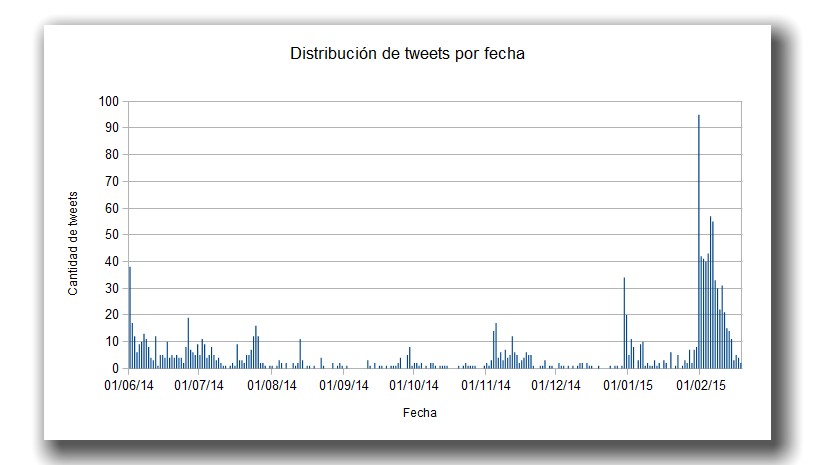
\includegraphics[width=1\textwidth]{imgs/123_general.png}
	\caption{Distribución de cantidad de tweets por día}
	\label{fig:123_tweets_por_dia}
\end{figure}

\begin{figure}[H]
	\centering
	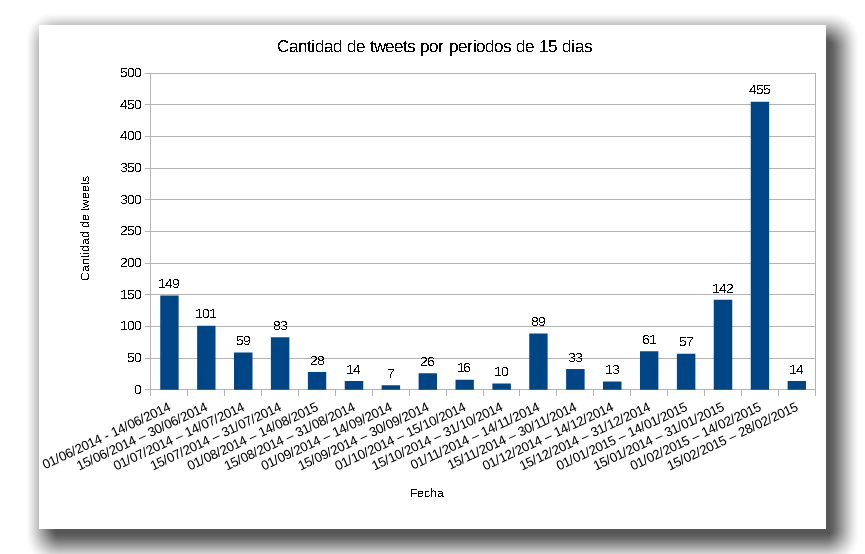
\includegraphics[width=1\textwidth]{imgs/cantidad_tweets_por_quincena_123_2.png}
	\caption{Distribución de cantidad de tweets por periodos de quince días}
	\label{fig:cantidad_tweets_por_quincena_123}
\end{figure}

En el gráfico \ref{fig:123_tweets_por_dia} es posible analizar la concentración de tweets por fecha, que en complemento del gráfico \ref{fig:cantidad_tweets_por_quincena_123} Nos permiten observar que existe una gran concentración de tweets en la primera quincena de febrero 2015 que se puede relacionar con la concentración de cuatros hitos noticiosos ocurridos desde el 1 de febrero hasta el 9 de febrero (ver tabla \ref{table:123_hitos_noticiosos}). El segundo periodo con más tweets corresponde a la primera quincena donde ocurrió un hito noticioso el 2 de junio de 2014. El tercer periodo con más tweets contiene un hito noticioso.(y dos hitos cercanos del periodo anterior, puesto que ocurrieron dos días antes del día previo del término del periodo). 

Es posible observar entonces que el debate se activa (y aumenta la cantidad de producción de tweets relacionados) en la medida que ocurren hechos noticiosos relevantes a nivel nacional.

\subsubsection{Análisis de re-tweet}

\begin{figure}[H]
	\centering
	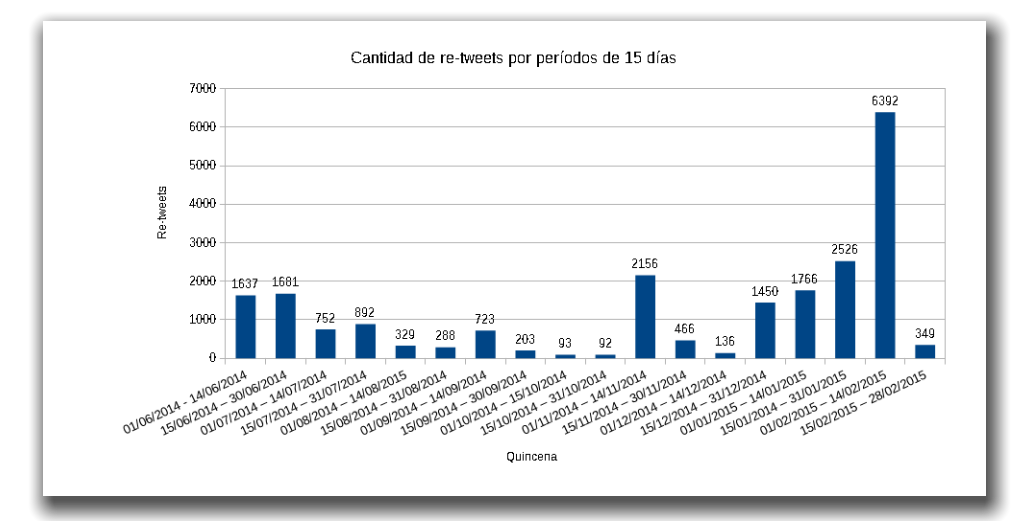
\includegraphics[width=1\textwidth]{imgs/123_cantidad_rt_por_quincena.png}
	\caption{Cantidad de re-tweets por quincena}
	\label{fig:123_cantidad_por_fecha}
\end{figure}

En el gráfico \ref{fig:123_tweets_por_dia} es posible analizar la concentración de tweets por periodo de tiempo, separados por quincena, el periodo de mayor concentración de tweets ocurre en la quincena 17 de manera similar a la mayor concentración de tweets analizados anteriormente, la segunda concentración ocurre en la segunda quincena de enero 2015  donde ocurre un hito noticioso, mientras que la tercera mayor concentración se ubica en la primera quincena del mes de noviembre 2014, donde se ubica un hito noticioso.

Según el razonamiento desarrollado para el \emph{ranking} de relevancia en ~\ref{subsubsec:orden-rel}. Los tweets con más RT son los que presentan información útil o relevante para quienes leyeron esos mensajes y realizaron la acción de re-tweet.

\begin{table}[H]
	\centering
	\begin{tabular}{| l | c | p{10cm} |}
		\hline
		Nº RT    & Autor & Texto de contenido\\ \hline
		1086  & @bairdCampbell & RT @fromerod: Los que prohibían el aborto,abortaban en  Londres.Hoy,quienes prohíben la libertad de expresión,se expresan en París. \\ \hline
		664  & @RosarioAlcaldeG & RT @joseantoniokast: Senador Lagos Weber tildo d "rasca" volante d la UDI sobre el aborto. Viendo esta foto sólo decir: Mira quien habla !  \\ \hline
		629  & @MAURYZS & RT @biobio: ONU recomienda a Chile permitir aborto a menores de 18 años por “salud fisiológica y mental” \\ \hline
		588  & @Beriiitha & RT @jmfmoran: Es menor, fue violada, quedó embarazada, no puede pagar un aborto, es obligada a parir un feto inviable. ¿Cuántas formas de v... \\ \hline
		360  & @raul\_torres79 & RT @link\_anarquista: Chile:Niña de 13 años embarazada por violación es castigada por el Estado sin derecho a aborto \\ \hline
		332  & @csuarezespinoza & RT @DerechaTuitera: Levantemos la mano todos los que creemos que el aborto provoca daños sicológicos irreparables! (acá un ejemplo) http \\ \hline
		253  & @RuubiaNaturaal & RT @lasultimas: Van Rysselberghe:"El aborto terapéutico es un control de calidad a la raza humana". Envía "weona loca" al 6969 y recibe chi \\ \hline
		252  & @urpiestrada & RT @PorAbortoLegal: Quién decide sobre un \#Aborto? explicación sencilla  http://t.co/cP4ApMZw33 \#provida \\ \hline
		243  & @irutherf & RT @KennethOficial: ¡Que ironía! Los que están a favor del aborto... nacieron. \\ \hline
		242  & @zarasenda & RT @SomosDocumental: Cine militante y documental contra la reforma de la Ley del aborto. http://t.co/NDfoNF4ABM \#TrendelaLibertad \\ \hline
	\end{tabular}
	\caption {10 Tweets mas re-twiteados del tópico}
	\label{table:123_topten_rt}
\end{table}

Si analizamos los tweets en \ref{table:123_topten_rt} es posible observar que 7 de los 10 cuentan con una imagen adjunta al tweet. De éstos 4 se refieren a un hecho noticioso, 4 se refieren a opiniones personales, 1 aporte a la discusión y 1 correspondiente a información internacional sobre el tema. 

\begin{table}[H]
	\centering
	\begin{tabular}{| c | c |}
		\hline
		\multicolumn{1}{|p{3cm}|}{Número de tweets emitidos por un mismo usuario} & \multicolumn{1}{p{3cm}|}{Número de usuarios  distintos} \\ \hline
		1 & 602 \\ \hline
		2 & 130 \\ \hline
		3 & 41  \\ \hline
		4 & 27 \\ \hline
		5 & 4  \\ \hline
		6 & 9  \\ \hline
		7 & 4  \\ \hline
		8 & 3  \\ \hline
		9 & 1  \\ \hline
		10 & 2  \\ \hline
		11 & 3  \\ \hline
		12 & 1  \\ \hline
		15 & 1  \\ \hline
		16 & 2  \\ \hline
		17 & 1  \\ \hline
	\end{tabular}
	\caption {Cantidad de usuarios distintos por número de tweets emitidos}
\end{table}

\subsubsection{Análisis geográfico}

La distribución de usuarios que realizaron tweets en el tópicos, con una ubicación 
identificada fueron 223 de los 831 autores distintos (26,8\%). De los cuales 20 se ubican en Antofagasta, 153 en Santiago, 

\begin{figure}[H]
	\centering
	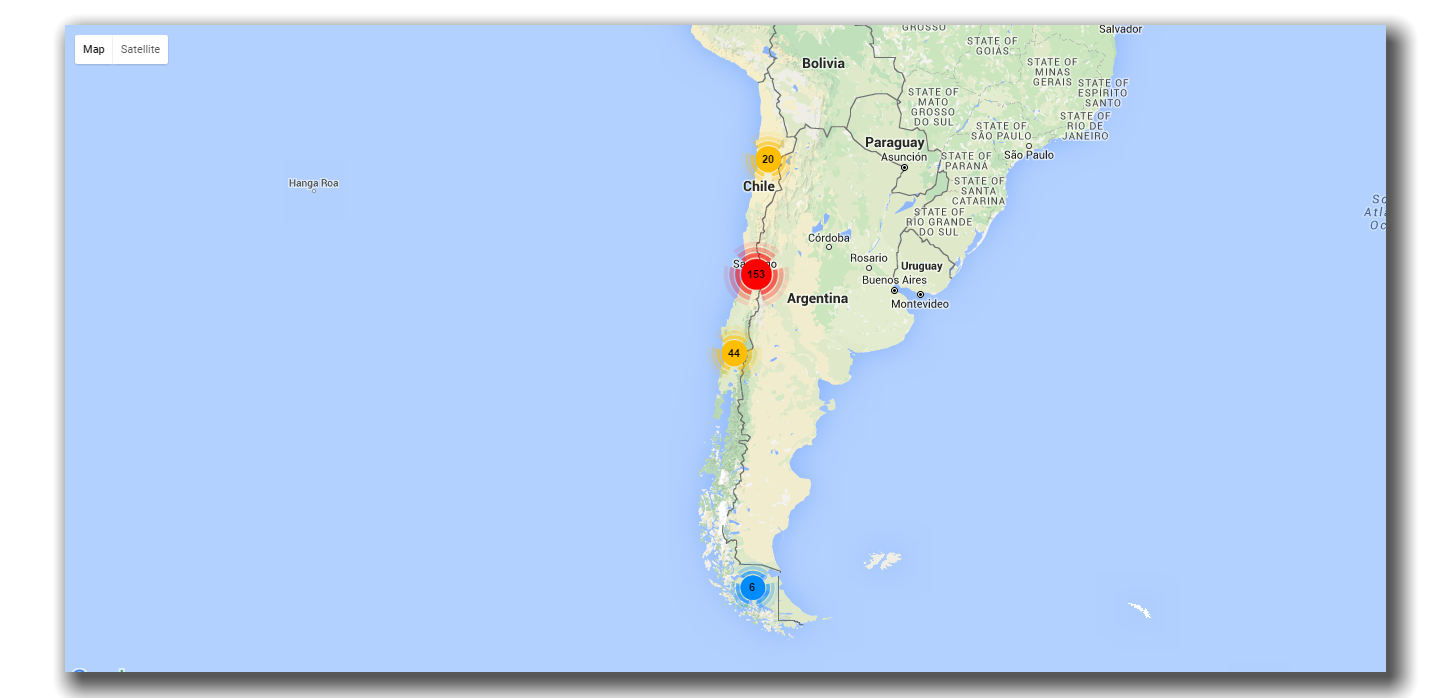
\includegraphics[width=1\textwidth]{imgs/213_usuarios_mapa.png}
	\caption{Distribución geográfica de los usuarios}
	\label{fig:geo_usuarios_213}
\end{figure}



	
	\chapter{Conclusiones}\label{chap:conclusiones}
	
		\section{Conclusiones}
		\subsection{Conclusiones técnicas}

El presente trabajo abarca aspectos teóricos y prácticos sobre la problemática
de informarse sobre un evento noticioso y profundiza en el desarrollo de una algoritmo computacional que recolecta información desde Twitter y la presenta en una interfaz web, con varias alternativas de presentación de la información.

La interfaz del prototipo posee una barra superior que de manera simple permite acceder a las distintas vistas de ordenamiento de los tweets y enlaces. Los tweets se presentan de manera descendente en una línea de tiempo con enlaces directos tanto al perfil del autor como a los distintos tweets facilitando el acceso directo a la fuente original, entregando una experiencia simple e intuitiva.

En la sección \ref{chap:estadodelarte} se analizan los distintos trabajos realizados sobre Twitter que tuvieran relación con aspectos abarcados en este trabajo tanto en estudios teóricos existentes como herramientas de fines similares. De forma general, la cantidad crecientes de estudios sobre Twitter permite verificar el creciente interés de la comunidad científica sobre esta red social.

Muchos de los trabajos revisados abordan de distinta manera la categorización de la información para dar solución a la problemática del valor de la información frente a los grandes volúmenes de Twitter. Para la clasificación de usuarios las estrategias variaban en la consideración de distintas características relacionadas a los tweets o a los usuarios en la plataforma, las más efectivas fueron aplicadas completa o parcialmente para el diseño de este prototipo. La revisión de las herramientas existentes actualmente permiten evidenciar la emergente industria de las aplicaciones que buscan recoger y presentar los contenidos de las redes sociales con variados objetivos entre los que se encuentran: monitoreo de opiniones sobre una marca, lectura resumida de las publicaciones de los contactos de un usuario en las redes sociales, mostrar información de tendencia, búsqueda de tweets o comprobación de la veracidad de la información.

Tras analizar los estudios referentes al geoposicionamiento de los usuarios fue posible evidenciar las dificultades respecto a este tema: sólo cerca del 20\% de los usuarios completan el campo ubicación del perfil, el resto lo completan con lugares muy generales o ficticios. Esta dificultad acotó las expectativas del prototipo de poder privilegiar las fuentes geográficamente más cercanas al lugar del hecho noticioso. El método implementado en este trabajo logra relacionar sólo el 17,54\% de los usuarios totales con una provincia específica de Chile. Existen variadas técnicas utilizadas para mejorar este relacionamiento en los diversos estudios analizados  \cite{Cheng:2010:YYT:1871437.1871535} \cite{McGee:2011:GST:2063576.2063959} pero debido a su complejidad se pretende abordar como desarrollo futuro.

Otra de las dificultades enfrentadas fueron los límites para la obtención de datos impuestos por la API de Twitter, estas limitaciones afectaron en el periodo de tiempo necesario para recolectar datos. 

%Una de las dificultades enfrentadas más relevantes fue la falta de estudios relacionados al uso de Twitter y al periodismo en las redes sociales enfocados en el territorio Chile. Esta dificultad fue enfrentada mediante el uso de bibliografía relacionada a otros medios de difusión disponibles en blogs y notas de prensa y en experimentos sobre el conjunto de datos recogidos.

En la sección \ref{sec:definicion_problema} pudimos profundizar en el interesante y activo debate sobre la influencia real en el usuario y en la construcción de una noticia de los procesos de \emph{gatekeeping}. El grado del impacto en el usuario depende de múltiples variables, entre ellas el ejercicio propio de informarse de cada persona que se dispone a informarse sobre un suceso noticioso. Una visión interesante es la que plantea Ramonet en \cite{fatigaInformarse} referente a que el ejercicio de informarse seriamente requiere esfuerzo y es una ilusión conseguirlo de manera cómoda, como supone la televisión. Es preciso para aprehender toda la complejidad de un suceso recordar los datos fundamentales de un problema, sus antecedentes históricos y su trama social y cultural. Esa misma filosofía sobre informarse, es la que da forma al prototipo al reunir en un mismo espacio comentarios, visiones y opiniones de distintas usuarias y usuarios ordenados y tratados con procesos de \emph{gatekeeping} transparentes además una lista de enlaces externos donde profundizar o complementar puntos de vistas recogidos de múltiples y variadas fuentes. Estos mismos aspectos abren interrogantes sobre la fortaleza de la arquitectura del prototipo desarrollado ¿no es acaso una debilidad importante que solo cuente con una fuente de información como es Twitter? ¿no se expone a caso al \emph{gatekeeping} proporcionado por Twitter?

Aún cuando Twitter, es una de las pocas redes sociales que trabaja constantemente en sus políticas de transparencia ( respecto a las solicitudes de información por parte de los gobiernos)  y plantean abiertamente una postura de transparencia frente a estos asuntos \footnote{``Creemos que el intercambio abierto de información puede tener un impacto global positivo. Para ello, es vital para nosotros (y otros servicios de Internet) para ser transparentes acerca de las solicitudes del gobierno para la información del usuario y de las solicitudes del gobierno para retener contenido de internet, el crecimiento de estas investigaciones pueden tener un efecto negativo grave en la libertad de expresión con implicaciones reales en la privacidad de las personas'' \cite{tweetsStillMustFlow} }, existen precedentes de decisiones comerciales-estratégicas que poseen componentes de censura.

\begin{itemize}
	\item \textbf{Intereses comerciales} como es el caso del bloqueo parcial a 
		Meerkat\footnote{Aplicación que permite realizar streaming de vídeo directamente a los seguidores del usuario en Twitter} competencia directa y de alto grado de utilización, competidora de Periscope, empresa comprada recientemente por Twitter para realizar streaming de vídeo. 
	\item \textbf{Políticas de uso}, como la denegación de acceso a la API para 
		Politwoops\cite{Diplotwoops:Online}, aplicación que hacía visible tweets borrados de políticos en más de 30 países. La cual Twitter justificó de la siguiente manera: "Imagínese: ¿Cómo sería de estresante- o incluso terrorífico-  twittear si fuera irrevocable o inalterable? Ningún usuario es más merecedor de esa capacidad que otro. De hecho, la eliminación de un tweet es una expresión del usuario".
	\item \textbf{Contexto y regulaciones culturales} como es el caso de los sistemas de filtros reactivos (sobre cuentas o tweets) que aplica Twitter para restricciones legales y culturales de los distintos países (escondiendo esos contenidos en sus respectivos países pero dejándolos disponibles en el resto del mundo) \cite{tweetsStillMustFlow}.
\end{itemize}

Considerando lo anterior, con una arquitectura que depende de una sola fuente de información el prototipo se expone a filtros de información ejecutados por esta fuente, que aún cuando sean transparentados verbalmente, es complejo verificar su real impacto sino no existe posibilidad de acceder al código fuente en cuestión. 

Otro aspecto interesante abordado en \ref{sec:definicion_problema} es referente a la discusión sobre de las razones de la existencia para los procesos de \emph{gatekeeping}. Una parte importante de autores sostienen que estos filtros son intencionados y diseñados con el objetivo de moldear la realidad que se trasmite mientras que otro grupo sostiene que éstos no son intencionales sino necesarios y de origen netamente operativo. En este trabajo, aún cuando se evitaron aplicar deliberadamente filtros de contenidos (de naturaleza editorial o ideológica), fue necesario - debido a la gran cantidad de datos disponibles - generar clasificaciones y selecciones para extraer y presentar la información relevante, sin estos tratamientos (debido a la gran cantidad de tweets recogidos) éstos carecen de valor. Considerando esta situación, se considera que la única solución coherente a esta situación es transparentar los procesos de \emph{gatekeeping} a sus usuarios, exponiendo de qué forma actúan y cómo se aplican, de esta manera los usuarios podrán verificar el real efecto que implican en un medio. A modo de metáfora, si tuviéramos la oportunidad de abrir las salas de prensas a miles de auditorías ciudadanas libres, éstas podrían verificar y corroborar las etapas de \emph{gatekeeping} de dicha sala de prensa y validarlas para generar confianza.

Respecto a los resultados encontrados fue posible verificar que Twitter es una fuente rica en información para la elaboración de reportes de un hecho noticioso, que no sólo sirve como herramienta de periodistas en la construcción de noticias sino que ha cambiado sus dinámicas y relación con los usuarios-consumidores de noticias. Los procesos aplicados a los tweets aportan valor en la medida que permiten extender la comprensión de un hecho noticioso.

El ejercicio de informarse sobre los hechos noticiosos es fundamental para la generación de opinión ciudadana, una herramienta como la presentada, contribuye a esta labor en cuanto facilita el acceso a informaciones difundidas por otras y otros ciudadanos y pone a sus disposición un reporte de opiniones, puntos de vistas y enlaces de documentación complementarios. 

%	\item \textit{Basado en el contenido}: Se refiere a las características relativas al contenido del tweet: novedad del tweet (distancia coseno de términos de los otros tweets que aparecen en el timeline en la última semana) y lo inesperado del tweet (distancia mínima de la distancia coseno de términos con los demás tweets del autor).

\subsection{Discusión sobre las conclusiones}


		
		\section{Trabajo futuro}
		El presente trabajo posee algunas componentes que podrían ser mejoradas para profundizar y mejorar aún más los resultados obtenidos. A continuación se presentan los distintos aspectos considerados para desarrollos futuros:

Referente al geoposicionamiento de las y los usuarios y su escasa tasa de llenado del campo \emph{ubicación} en sus perfiles, se considera necesario desarrollar enfoques con mejores resultados considerando no sólo datos relativos a los usuarios sino al contenidos de los tweets (Como el abordado en \cite{Cheng:2010:YYT:1871437.1871535} \cite{doi:10.1080/00330124.2014.907699} \cite{Dredze_carmen:a} \cite{GraellsGarridoP13}). Un enfoque interesante de analizar es la identificación de hashtags locales y palabras locales, fortaleciéndolo con temáticas exclusivas y delimitadas a dicha zona, para identificar y relacionar tweets con esa zona geográfica específica.

	En cuanto al desempeño del prototipo se pueden realizar importantes mejoras. Una de las opciones más atractivas respecto a la mejora de su arquitectura (relación rendimiento, escalabilidad y precio) es incorporar algunos de los Servicios Web de Amazon (AWS). 
	
	AWS son el conjunto de servicios escalables tanto en costos como en capacidad que ofrece Amazon, permitiendo el acceso a hardware de alto desempeño y la automatización de procesos a un costo accesible (ver anexo \ref{sec:cotizacionAmazon}). Entre los servicios que  ofrece se encuentran: cómputo global, almacenamiento, bases de datos, análisis, aplicaciones e implementación de servicios.
	
	Los servicios que pueden contribuir directamente a mejorar el desempeño del prototipo son los siguientes:
	
	\begin{itemize}
		\item \textbf{Amazon RDS}: Proporciona un servicio seguro, escalable y simple de administrar para bases de datos en la nube. Proporcionando una capacidad rentable y de tamaño variable ante posibles crecimientos. AWS RDS proporciona seis motores de base de datos entre los que se encuentran MySQL.
		
		Incorporar este servicio mejoraría sustancialmente el proceso actual de acceso a los datos para su análisis y eliminando las limitaciones de almacenamiento de datos. Su uso estaría destinado para almacenar los datos captados desde Twitter mediante la API y transferir conjuntos de datos a la base de datos cada cierta unidad de tiempo, para su almacenamiento permanente.
		
		\item \textbf{Amazon Kinesis}: Proporciona un servicio de procesamiento de datos en tiempo real a streaming de gran cantidad de datos. Amazon Kinesis puede capturar continuamente y almacenar terabytes de datos por hora a partir de cientos de fuentes de datos.
		
		La incorporación de este servicio puede contribuir significativamente en la reducción de tiempos que toman las distintas fases del procesamiento de los datos para la creación de un nuevo tópico abriendo también una increíble oportunidad de  re-estructuración completa del proceso de captación de tweets, migrando  la captación desde la API REST de Twitter (con el análisis post del conjunto de tweets) a la captación de tweets desde la API STREAMING de Twitter (aplicando el análisis en tiempo real), aumentando considerablemente la frescura de la información ofrecida por el prototipo.
		
		\item \textbf{Amazon Elastic Compute Cloud (EC2)}: Es un servicio web que proporciona capacidad de cálculo escalable en la nube. EC2 cuenta con una interfaz fácil de uso que entrega un control completo de los recursos informáticos, entregando la posibilidad de arrancar nuevas instancias de servidor en segundos, permitiendo escalar rápidamente la capacidad a medida que cambian las necesidades.
		
		Estas posibilidades repercuten directamente en los tiempos de respuesta de las distintas fases del análisis del prototipo como la aplicación del clasificador, la recolección de enlaces, el orden de los distintos rankings entre otros, aumentando la capacidad de generación de los diversos tópicos.
		
	\end{itemize}
	
En la sección previa referente a las conclusiones se plantea la importancia de la trasparencia en los distintos procesamientos que se aplican a la información en la construcción de una noticia, es por ello, que un trabajo a futuro relevante es la habilitación de este prototipo para uso y la disposición ante la comunidad del código fuente desarrollado. La habilitación de este prototipo de un servidor de acceso público fue descartado como desarrollo de este trabajo debido a la inviabilidad económica de su mantención a mediano-largo plazo.
	
Otro aspecto relevante observado durante el desarrollo de este trabajo es el bajo volumen de documentación existente sobre hábitos de consumo de información y comportamiento para informarse en territorio nacional mediante internet o las redes sociales. Por lo cual, un interesante trabajo a futuro es perfilar y obtener información que permitan caracterizar a la población de usuarios de Twitter en Chile, esta información irá en directo beneficio para la comunidad de desarrolladores e investigadores sobre la materia en territorio nacional. 

Bajo esta misma perspectiva, y considerando el principal enfoque de diseño de Storyful “vivir dentro de las comunidades de medios sociales, no para observar desde una distancia segura" sería interesante incorporar componentes participativas en el prototipo  de tal manera que los mismos ciudadanos puedan contribuir a la divulgación y generación de información, en un esquema democrático y sin preferencias ni discriminaciones arbitrarias. En el último tiempo, los medios de prensa han incluido reportes de noticias ciudadanas de manera parcial (ya que sólo se limita a utilizar el material proporcionado por el reporte, sin incluir componentes sociales del usuario, comentarios de éste u información deducida en base a la interacción con el círculo humano con la intención de profundizar en la situación presentada), habilitando un número de contacto donde se pueden enviar videos a través de Whatsapp o Twitter,

	%desempeño en la captura de tweets
	%desempeño en el analisis de un conjunto para un topico
	
	%subir a un servidor de produccion para obtener métricas de uso y mejoras basadas en el uso frecuente
	
	%mejora en el metodo de busqueda de tweets mediante conjuntos selectivos de generadores de reportes.

	%Estudiar hábitos que tienen los chilenos al informarse desde sus dispositivos moviles como notebooks, smarthphone, tables.
	
	%Se pretende además incluir componentes de periodismo ciudadano en esta herramienta del siguiente modo: el observador directo de un evento o quien pretenda replicar una información generalmente busca visibilidad de su mensaje tweeteando a un usuario de mayor popularidad como algún medio noticioso tradicional y de amplia audiencia. Se incluirán estos mensajes además de los reportes directos que se realicen al tweet de la herramienta planteada.

	
	\chapter{Anexo}\label{chap:anexo}
	\section{Cuentas en Twitter de los medios de prensa}

\begin{center}
	\centering
		\begin{longtable}{| l | c | c | c |}
		%\label{table:anpMedios}
		\hline
			Medio de prensa    & Usuario  & Nº amigos & Nº seguidores \\ \hline	
40 Principales - Copiapó	&	@40ChileOficial	&	702	&	174K	\\ \hline
40 Principales - Isla de Pascua	&		&		&		\\ \hline
40 Principales - Osorno	&		&		&		\\ \hline
40 Principales - Puerto Montt	&		&		&		\\ \hline
40 Principales - Rancagua	&		&		&		\\ \hline
40 Principales - San Antonio	&		&		&		\\ \hline
40 Principales - Talca	&		&		&		\\ \hline
40 Principales - Temuco	&		&		&		\\ \hline
40 Principales - Villarrica	&		&		&		\\ \hline
Agricultura - Los Angeles	&	@agriculturafm	&	2407	&	40,4K	\\ \hline
Agrovision Fm	&		&		&		\\ \hline
Antofagasta Televisión	&	@antofagastatv	&	1107	&	18,4K	\\ \hline
Autentica - Frutillar	&		&		&		\\ \hline
Autentica - Rengo	&		&		&		\\ \hline
Bravo	&	@RadioBravoFM	&	37	&	87	\\ \hline
Carolina - Viña Del Mar	&	@RadioCarolina	&	15	&	358K	\\ \hline
Chilena - Santiago	&	@RadioChilena	&	44	&	70	\\ \hline
comunicaciones zona Fm	&		&		&		\\ \hline
Cooperativa - Ancud	&		&		&		\\ \hline
Cooperativa - Angol	&		&		&		\\ \hline
Cooperativa - Arauco	&		&		&		\\ \hline
Cooperativa - Calama	&		&		&		\\ \hline
Cooperativa - Caldera	&		&		&		\\ \hline
Cooperativa - Casablanca	&		&		&		\\ \hline
Cooperativa - Chillán	&		&		&		\\ \hline
Cooperativa - Constitución	&		&		&		\\ \hline
Cooperativa - Copiapó	&		&		&		\\ \hline
Cooperativa - Curicó	&		&		&		\\ \hline
Cooperativa - Iquique	&		&		&		\\ \hline
Cooperativa - Linares	&		&		&		\\ \hline
Cooperativa - Los Vilos	&		&		&		\\ \hline
Cooperativa - Mulchen	&		&		&		\\ \hline
Cooperativa - Ovalle	&		&		&		\\ \hline
Cooperativa - Puerto Aysén	&		&		&		\\ \hline
Cooperativa - San Antonio	&		&		&		\\ \hline
Cooperativa - San Felipe	&		&		&		\\ \hline
Cooperativa - Santiago	&		&		&		\\ \hline
Cooperativa - Talca	&		&		&		\\ \hline
Cooperativa - Temuco	&		&		&		\\ \hline
Cooperativa - Tocopilla	&		&		&		\\ \hline
Cooperativa - Valdivia	&		&		&		\\ \hline
Cooperativa - Vallenar	&		&		&		\\ \hline
Cordialissima	&		&		&		\\ \hline
Crystal	&		&		&		\\ \hline
Crystal - La Ligua	&		&		&		\\ \hline
Crystal - Quillota	&	@RadioCrystalQTA	&	181	&	160	\\ \hline
Cumbre	&	RadioCumbreFM	&	103	&	162	\\ \hline
Dalcahue	&	DigitalFMChile	&	1617	&	3846	\\ \hline
Digital Fm - La Serena	&		&		&		\\ \hline
El Conquistador - Santiago	&	FMConquistador	&	193	&	31,4K	\\ \hline
En Voz Alta	&		&		&		\\ \hline
Enamorada	&		&		&		\\ \hline
Entre Ríos	&	ENTRERIOSRADIO	&	113	&	46	\\ \hline
Estación 106	&		&		&		\\ \hline
Eva Fm	&	radioevafm	&	1130	&	1263	\\ \hline
Festival	&	radio\_festival	&	1292	&	24,1k	\\ \hline
Fm Contigo Tus Clasicos - Caldera	&		&		&		\\ \hline
Fm Dos - San Felipe	&	FMDOS	&	251	&	56,4k	\\ \hline
Fm Okey - Los Andes	&	FMOK	&	1812	&	6730	\\ \hline
Gaminides	&		&		&		\\ \hline
Hotel Cordillera	&		&		&		\\ \hline
Imagina - San Felipe	&		&		&		\\ \hline
Imagina - Santiago	&	imagina881	&	1285	&	4474	\\ \hline
Imaginación Fm	&	imaginacionFM	&	276	&	182	\\ \hline
Impacto - Calama	&		&		&		\\ \hline
Indomita	&		&		&		\\ \hline
Infinita - Los Angeles	&	infinitafm	&		&		\\ \hline
Infinita - Puerto Montt	&		&	307	&	10,2k	\\ \hline
Lincoyan	&		&		&		\\ \hline
Los Confines	&		&		&		\\ \hline
Madero Fm	&	radiomaderofm	&	4480	&	8445	\\ \hline
Mágica - Talca	&		&		&		\\ \hline
Manantial Fm - talagante	&	MANANTIALtlgte	&	106	&	488	\\ \hline
Mi Radio - Paillaco	&		&		&		\\ \hline
Nueva Fm Super Stereo	&		&		&		\\ \hline
Nueva Maule	&		&		&		\\ \hline
Nuevo Mundo	&	RNuevoMundo	&	4673	&	9247	\\ \hline
Onda Fm	&		&		&		\\ \hline
Parinacota	&		&		&		\\ \hline
Pudahuel - Los Andes	&	RadioPudahuel	&	20,1k	&	25,2k	\\ \hline
Radio Acogida	&		&		&		\\ \hline
Radio Aconcagua	&	aconcaguaradio	&	117	&	5839	\\ \hline
Radio Aconcagua A.M y F.M	&		&		&		\\ \hline
Radio Actual Fm	&		&		&		\\ \hline
Radio Agricultura - Santiago	&	agriculturafm	&	2405	&	36,4k	\\ \hline
Radio Almeyda Fm	&		&		&		\\ \hline
Radio Ambrosio	&		&		&		\\ \hline
Radio Ambrosio Linares	&	ambrosiofm	&	27	&	1055	\\ \hline
Radio Amiga	&	radio\_amiga	&	14	&	583	\\ \hline
Radio Anahí	&	RADIOANAHICHILE	&	372	&	217	\\ \hline
Radio Angel	&	RADIOANGEL3	&	90	&	79	\\ \hline
radio Antares	&		&		&		\\ \hline
Radio Apocalipsis	&	fmapocalipsis	&	960	&	754	\\ \hline
Radio Araucana	&		&		&		\\ \hline
Radio Artesanía	&	ARTESANIAFM	&	526	&	329	\\ \hline
Radio Atractiva Fm	&	radioatractiva	&	892	&	1320	\\ \hline
Radio Austral	&		&		&		\\ \hline
Radio Ayer - Rio Negro	&	Radio\_Ayer	&	499	&	263	\\ \hline
Radio Azul	&		&		&		\\ \hline
Radio Bahia - Taltal	&	Bahia\_Radio	&	50	&	160	\\ \hline
Radio Balneario	&		&		&		\\ \hline
Radio Beethoven 96,5 F.M.	&	radiobeethoven	&	3804	&	3888	\\ \hline
Radio Bravissima F.M. Digital Stereo	&		&		&		\\ \hline
Radio Buena Nueva	&	RadioBuenaNueva	&	232	&	2412	\\ \hline
Radio Buena Onda	&	radiobuenaonda	&	35	&	68	\\ \hline
Radio Calama	&		&		&		\\ \hline
Radio Camila - Limache	&		&		&		\\ \hline
Radio Camila - Los Angeles	&	983camila	&	2	&	139	\\ \hline
Radio Canal 95	&	canal95	&	376	&	2862	\\ \hline
Radio Candelaria	&		&		&		\\ \hline
Radio Canelo 149 Am.	&		&		&		\\ \hline
Radio Cappissima	&	cappissima	&	195	&	923	\\ \hline
Radio Caribe FM	&	caribefm	&	63	&	185	\\ \hline
Radio Caricia	&		&		&		\\ \hline
Radio Carillon	&	radiocarillon	&	24	&	140	\\ \hline
Radio Carnaval	&	Carnaval\_FM	&	106	&	4034	\\ \hline
Radio Carnaval - Ovalle	&		&		&		\\ \hline
Radio Carnaval - San Felipe	&	Carnaval\_FM	&		&		\\ \hline
Radio Carolina - San Antonio	&		&		&		\\ \hline
Radio Carolina - Temuco	&		&		&		\\ \hline
Radio Carolina - Villarrica	&		&		&		\\ \hline
Radio Carolina Santiago	&	RadioCarolina	&	15	&	358K	\\ \hline
Radio Centenario	&		&		&		\\ \hline
Radio Centinela	&	RadioCentinela	&		&	231	\\ \hline
Radio Cobre Mar	&	cobremar\_radio	&	303	&	185	\\ \hline
Radio Colchagua	&		&		&		\\ \hline
Radio Comunicativa	&	radcomunicativa	&	1149	&	2313	\\ \hline
Radio Condell	&	radiocondell	&	4482	&	10,1K	\\ \hline
Radio Conifera	&		&		&		\\ \hline
Radio Contigo Fm	&	RadioContigoFm	&	2003	&	1240	\\ \hline
Radio Copihue	&		&		&		\\ \hline
Radio Cultural	&		&		&		\\ \hline
Radio Del Lago	&		&		&		\\ \hline
Radio Desierto	&	desiertofm	&	1616	&	4366	\\ \hline
Radio Difusora Dinámica Ltda.	&	radio\_dinamica	&	780	&	1781	\\ \hline
Radio Digital	&	DigitalFmChile	&	1618	&	3847	\\ \hline
Radio Digital Fm - Diego de Almagro	&		&		&		\\ \hline
Radio Dinámica - Iquique	&		&		&		\\ \hline
Radio Duna - Viña Del Mar	&	RadioDuna	&	579	&	67,1K	\\ \hline
Radio El Conquistador - Iquique	&		&		&		\\ \hline
Radio El Faro FM.	&		&		&		\\ \hline
Radio El Mundo	&		&		&		\\ \hline
Radio Ensenada Fm	&		&		&		\\ \hline
Radio Entrevalles	&		&		&		\\ \hline
Radio Esperanza - Temuco	&	esperanzafm	&	238	&	303	\\ \hline
Radio Estrella Del Norte	&	estrelladelno	&	359	&	231	\\ \hline
Radio Exodo	&		&		&		\\ \hline
Radio Fiessta	&	fiessta909	&	1197	&	5383	\\ \hline
Radio Fm Mix	&		&		&		\\ \hline
Radio FM Plus	&		&		&		\\ \hline
Radio Fm Siete (Formato Español)	&		&		&		\\ \hline
Radio Futura F.M. Stereo	&	futurafmoficial	&	2230	&	3617	\\ \hline
Radio Futuro - Punta Arenas	&	futurofm	&	710	&	148K	\\ \hline
Radio Genesis - Andacollo	&		&		&		\\ \hline
Radio Genoveva 101.7	&		&		&		\\ \hline
Radio Gratissima	&	RadioGratissima	&	737	&	1157	\\ \hline
Radio Guardia Marina Ernesto Riquelme	&		&		&		\\ \hline
Radio Horizonte	&	radiohorizonte	&	24,5K	&	76,1k	\\ \hline
Radio Horizonte - Antofagasta	&		&		&		\\ \hline
Radio Horizonte - Temuco	&		&		&		\\ \hline
Radio Ignacio Serrano	&		&		&		\\ \hline
Radio Imagina	&	imagina881	&	1286	&	4618	\\ \hline
Radio Integración	&		&		&		\\ \hline
Radio La Bruja FM	&		&		&		\\ \hline
Radio la Frontera	&		&		&		\\ \hline
Radio La Palabra	&		&		&		\\ \hline
Radio La Voz de La Costa	&	VozdelaCosta	&	1572	&	3333	\\ \hline
Radio la Voz de la Tierra A.M.	&		&		&		\\ \hline
Radio Lanco FM.	&	radioLancofm	&	56	&	49	\\ \hline
Radio Latina Fm	&		&		&		\\ \hline
Radio Lautaro	&	RadioLautaro	&	226	&	1380	\\ \hline
Radio Libra	&		&		&		\\ \hline
Radio Lógika	&	LogikaFM	&	1836	&	2910	\\ \hline
Radio Loncoche A.M.	&		&		&		\\ \hline
Radio Madrigal	&		&		&		\\ \hline
Radio Madrigal Fm	&		&		&		\\ \hline
Radio Malleco	&		&		&		\\ \hline
Radio Manía	&		&		&		\\ \hline
Radio Marcela	&		&		&		\\ \hline
Radio Maria	&	radiomariachile	&	284	&	1917	\\ \hline
Radio Maxima - Antofagasta	&		&		&		\\ \hline
Radio Mirador	&	Radiomiradorfm	&	1875	&	1409	\\ \hline
Radio Montecarlo - Iquique	&		&		&		\\ \hline
Radio Montecarlo - La Serena	&	montecarlocl	&	1100	&	3864	\\ \hline
Radio Montecarlo - Ovalle	&		&		&		\\ \hline
Radio Montecarlo - Valdivia	&		&		&		\\ \hline
Radio Montecarlo - Vicuña	&		&		&		\\ \hline
Radio Monumental	&		&		&		\\ \hline
Radio Nacimiento 98,7 F.M.	&		&		&		\\ \hline
Radio Nahuelbuta	&	radionahuelbuta	&	234	&	1042	\\ \hline
Radio Nativa	&	rad\_nativa	&	33	&	242	\\ \hline
Radio Nexo y Libra	&	radiolibraynexo	&	263	&	1716	\\ \hline
Radio Norte Verde	&		&		&		\\ \hline
Radio Nueva Belén	&	nuevabelenfm	&	330	&	1368	\\ \hline
Radio Nueve-Veinte	&		&		&		\\ \hline
Radio Nuevo Tiempo	&	ntchile	&	294	&	814	\\ \hline
Radio Oceania	&		&		&		\\ \hline
Radio Pablo Neruda	&		&		&		\\ \hline
Radio Paloma	&	RADIOPALOMAFM	&	1311	&	27K	\\ \hline
Radio Panamericana A.M.	&		&		&		\\ \hline
Radio Panorama	&		&		&		\\ \hline
Radio Parque Nacional A.M.	&		&		&		\\ \hline
Radio Paula Jaraquemada	&		&		&		\\ \hline
Radio Payne	&		&		&		\\ \hline
Radio Pewen FM	&	PEHUEN\_FM	&	35	&	84	\\ \hline
Radio Play FM - Antofagasta	&	play\_fm	&	635	&	41,9K	\\ \hline
Radio Play FM - Iquique	&		&		&		\\ \hline
Radio Play FM - La Serena	&		&		&		\\ \hline
Radio Play FM - Santiago	&		&		&		\\ \hline
Radio Portales Cb-118	&	RadioPortales	&	2302	&	8806	\\ \hline
Radio Primordial	&		&		&		\\ \hline
Radio Principal Chuquicamata	&		&		&		\\ \hline
Radio Progreso	&		&		&		\\ \hline
Radio Pudahuel - Santiago	&	RadioPudahuel	&	22,1K	&	26,9K	\\ \hline
Radio Puerta Norte	&		&		&		\\ \hline
Radio Pukara	&	RadioPukara981	&	144	&	108	\\ \hline
Radio Raudal	&	raudalfm	&	562	&	137	\\ \hline
Radio Renacer	&	Renacer1017	&	44	&	15	\\ \hline
Radio Rio Claro	&		&		&		\\ \hline
Radio Rio Elqui	&		&		&		\\ \hline
Radio Rock \& Pop - RANCAGUA	&	rockandpop	&	1119	&	84,2K	\\ \hline
Radio Rock \& Pop - SAN CLEMENTE	&		&		&		\\ \hline
Radio Romance	&		&		&		\\ \hline
Radio Romántica	&	Radio\_Romantica	&	147	&	18,7K	\\ \hline
Radio Romina	&		&		&		\\ \hline
Radio Sago	\&	RadioSago	&	1131	&	11K	\\ \hline
Radio San Bartolomé	&	rsboficial	&	653	&	5289	\\ \hline
Radio Santiago	&	radio\_santiago	&	732	&	5293	\\ \hline
Radio Sol	&	radiosolchile	&	1014	&	2243	\\ \hline
Radio Somos Pichilemu	&	somospichilemu1	&	1161	&	1169	\\ \hline
Radio Stellar Fm	&		&		&		\\ \hline
Radio Súper andina	&		&		&		\\ \hline
Radio Tiempo - Santiago	&	radiofmtiempo	&	1184	&	19,4K	\\ \hline
Radio Tiempo - Viña Del Mar	&		&		&		\\ \hline
Radio Topater	&	radiotopaterfm	&	476	&	141	\\ \hline
Radio Trasandina	&		&		&		\\ \hline
Radio Trigal F M Stereo 103 9 Mhz	&	trigal\_fm	&	249	&	1514	\\ \hline
Radio Univ. de Antofagasta	&	radiouantof	&	714	&	473	\\ \hline
Radio Universidad Austral	&		&		&		\\ \hline
Radio Universidad de Chile	&	uchileradio	&	2685	&	58,1k	\\ \hline
Radio Universidad de la Frontera	&	UfroRadioTemuco	&	45	&	2452	\\ \hline
Radio Universidad de Talca	&		&		&		\\ \hline
Radio Universitaria Fm	&	universitaria	&	1807	&	2108	\\ \hline
Radio Universo - Santiago	&	RadioUniverso	&	144K	&	132K	\\ \hline
Radio Ventisqueros - Chile Chico	&		&		&		\\ \hline
Radio Ventisqueros - Cochrane	&	Ventisqueros	&	91	&	1360	\\ \hline
Radio Viaducto	&	RadioViaducto	&	406	&	948	\\ \hline
Radio X - La Serena	&		&		&		\\ \hline
Radio X - Santiago	&		&		&		\\ \hline
Radio X - Viña Del Mar	&		&		&		\\ \hline
Radio xqa5	&		&		&		\\ \hline
Radio Zero S.A.	&	radiocero977	&	6561	&	61,8K	\\ \hline
Radioactiva - Castro	&	RadioActivaFm	&	1019	&	82,5K	\\ \hline
Radioactiva - Chillán	&		&		&		\\ \hline
Radioactiva - La Serena	&		&		&		\\ \hline
Radioactiva - Los Angeles	&		&		&		\\ \hline
Radioactiva - Osorno	&		&		&		\\ \hline
Radioactiva - Ovalle	&		&		&		\\ \hline
Radioactiva - Puerto Montt	&		&		&		\\ \hline
Radioactiva - Punta Arenas	&		&		&		\\ \hline
Radioactiva - Rancagua	&		&		&		\\ \hline
Radioactiva - San Antonio	&		&		&		\\ \hline
Radioactiva - San Felipe	&		&		&		\\ \hline
Radioactiva - Talca	&		&		&		\\ \hline
Radioactiva - Temuco	&		&		&		\\ \hline
Radioactiva - Valdivia	&		&		&		\\ \hline
RadioProyección	&	RadioProyeccion	&	397	&	602	\\ \hline
Radiovision	&	RadioVision997	&	14	&	23	\\ \hline
Rinconada Fm	&		&		&		\\ \hline
San Sebastian	&		&		&		\\ \hline
Sociedad Radiodifusora Monterrey Ltda.	&		&		&		\\ \hline
Tiempo - San Antonio	&		&		&		\\ \hline
Tornagaleones	&	TomagaleonesFM	&	33	&	105	\\ \hline
Ucv Televisión	&	ucv\_tv	&	188	&	19,1K	\\ \hline
Universidad de Santiago - Santiago	&	radiousach	&	3484	&	18,5K	\\ \hline
Universidad de Tarapaca - Arica	&		&		&		\\ \hline
Universo - Iquique	&		&		&		\\ \hline
Universo - Osorno	&		&		&		\\ \hline
Universo - Temuco	&		&		&		\\ \hline
W Radio - Ancud	&		&		&		\\ \hline
W Radio - Arica	&		&		&		\\ \hline
W Radio - Chillán	&		&		&		\\ \hline
W Radio - Copiapó	&		&		&		\\ \hline
W Radio - Isla de Pascua	&		&		&		\\ \hline
W Radio - La Serena	&		&		&		\\ \hline
W Radio - Linares	&		&		&		\\ \hline
W Radio - Los Angeles	&		&		&		\\ \hline
W Radio - Osorno	&		&		&		\\ \hline
W Radio - Ovalle	&		&		&		\\ \hline
W Radio - Parral	&		&		&		\\ \hline
W Radio - Puerto Aysén	&		&		&		\\ \hline
W Radio - Puerto Montt	&		&		&		\\ \hline
W Radio - Punta Arenas	&		&		&		\\ \hline
W Radio - Rancagua	&		&		&		\\ \hline
W Radio - San Antonio	&		&		&		\\ \hline
W Radio - San Felipe	&		&		&		\\ \hline
W Radio - Talca	&		&		&		\\ \hline
W Radio - Tierra Amarilla	&		&		&		\\ \hline
W Radio - Valdivia	&		&		&		\\ \hline
W Radio - Villarrica	&		&		&		\\ \hline
W Radio - Viña Del Mar	&		&		&		\\ \hline
Cooperativa	&	cooperativacl	&	507K	&	1,73M	\\ \hline
\caption {Medios de prensa ANP y características de sus cuentas en Twitter al 5 de junio del 2015.}
	\end{longtable}
\end{center}

\begin{center}
	\centering
	\begin{longtable}{| l | c | c | c |}
		
		%\label{table:anarchicMedios}
		\hline
			Medio de prensa    & Usuario  & Nº amigos & Nº seguidores \\ \hline	
			Cuarta Colina	&	cuartacolina	&	49	&	79	\\ \hline
			Radiovision	&	FmRadiovision	&	17	&	41	\\ \hline
			Radio Alas	&	Radioalas	&	1987	&	1444	\\ \hline
			Radio Vanguardia	&	fmvanguardia	&	1	&	52	\\ \hline
			Radio Creativa FM	&	RadioCreativaFM	&	11	&	180	\\ \hline
			Radio Puro Chile	&	radiopurochile	&	25	&	242	\\ \hline
			Radio Paloma	&	RADIOPALOMAFM	&	1308	&	26500	\\ \hline
			Radio Enlace Sur	&	Radioenlacesur	&	326	&	113	\\ \hline
			Radio Interferencia	&	interferenciafm	&	211	&	308	\\ \hline
			Casa Blanca	&	casablancafm	&	222	&	219	\\ \hline
			Radio Ritoque	&	RitoqueFM	&	642	&	5062	\\ \hline
			Radio Algarrobo	&	radioalgarrobo	&		&		\\ \hline
			La voz de Cerro Navia	&	lavozcerronavia	&	16	&	15	\\ \hline
			Radio Eclipse	&	radioeclipsefm	&	54	&	201	\\ \hline
			Radio Mater Dei	&	radiomaterdei	&	10	&	9	\\ \hline
			Radio Primavera	&	rprimaverafm	&	451	&	495	\\ \hline
			Radio Lorenzo Arenas	&	rlaradio	&	82	&	109	\\ \hline
			Radio Licanten	&	Radio\_Licanten	&	922	&	607	\\ \hline
			Radio Espacios FM	&	espaciosfm	&	143	&	144	\\ \hline
			Radio Nueva Dichato	&	NuevaDichato	&	128	&	735	\\ \hline
			Radio Paula	&	Radio\_Paula	&	28	&	115	\\ \hline
			Radio Pelom FM	&	RadioPelom	&	120	&	65	\\ \hline
			Radio Chiloé	&	radiochiloe	&	3140	&	8199	\\ \hline
			Radio Agricultura	&	agriculturafm	&	2405	&	39400	\\ \hline
			
		\caption {Medios de prensa pertenecientes a ANARCHIC y características de sus cuentas en Twitter al 5 de junio del 2015.}
		
	\end{longtable}
\end{center}

\begin{center}
	\centering
	\begin{longtable}{| l | c | c | c |} \hline
		Nombre del Medio	&	Screen Name	&	Siguiendo (Following)	&	Seguidores (Followers)	\\ \hline
		La estrella de Iquique	&	laestrellaiqq	&	462	&	17900	\\ \hline
		La estrella de Loa	&	estrella\_loa 	&	82	&	2266	\\ \hline
		La estrella de Antofagasta	&	estrella\_antofa 	&	150	&	8613	\\ \hline
		Mercurio de Antofagasta	&	mercurioafta	&	1751	&	21600	\\ \hline
		Diario Chañarcillo	&	chanarcillo	&	1964	&	6597	\\ \hline
		Diario Atacama	&	diarioatacama	&	65	&	8570	\\ \hline
		Diario el Día	&	eldia\_cl	&	580	&	38100	\\ \hline
		El Ovallino	&	elovallino	&	267	&	5851	\\ \hline
		Diario El Observador	&	eo\_enlinea	&	614	&	14100	\\ \hline
		La estrella de Quillota	&	laestrelladeqta	&	1847	&	6773	\\ \hline
		La estrella de Valparaiso	&	laestrellavalpo 	&	10	&	23800	\\ \hline
		Lider de San Antonio	&	lidersanantonio	&	289	&	7775	\\ \hline
		Diario el Labrador	&	diariolabrador	&	264	&	1600	\\ \hline
		Lider de Melipilla	&	lidermelipilla 	&	465	&	657	\\ \hline
		La nacion	&	nacioncl	&	4116	&	220000	\\ \hline
		La Tercera	&	latercera	&	224000	&	1110000	\\ \hline
		El Mercurio	&	Emol	&	503000	&	1030000	\\ \hline
		La cuarta	&	lacuarta	&	36800	&	533000	\\ \hline
		Diario Financiro	&	DFinanciero	&	192	&	82800	\\ \hline
		Diario La Hora	&	DiarioLaHora	&	10300	&	207000	\\ \hline
		El Pulso &	pulso\_tw	&	816	&	31600	\\ \hline
		La Segunda	&	La\_Segunda	&	3395	&	392000	\\ \hline
		El Rancaguino	&	elrancaguino	&	489	&	18400	\\ \hline
		La prensa de curicó	&	laprensacurico	&	1	&	5306	\\ \hline
		Diario El Centro	&	diarioelcentro	&	2333	&	22300	\\ \hline
		Diario Heraldo	&	Heraldo\_Diario	&	9	&	131	\\ \hline
		Cronica de Chillán	&	CronicaChillan	&	88	&	17800	\\ \hline
		La discusión	&	ladiscusioncl	&	1409	&	19100	\\ \hline
		El Sur	&	elsurcl	&	645	&	26700	\\ \hline
		Diario Concepción	&	DiarioConce	&	1152	&	14300	\\ \hline
		La Tribuna	&	latribunacl	&	643	&	3354	\\ \hline
		El Austral	&	AustralTemuco	&	2255	&	40500	\\ \hline
		El Austral de los Rios	&	austral\_losrios	&	12	&	11700	\\ \hline
		El Austral de Osorno	&	austral\_osorno	&	1128	&	15400	\\ \hline
		La Estrella de Chiloé	&	estrellachiloe	&	94	&	8424	\\ \hline
		El Austral	&	ellanquihue	&	747	&	20500	\\ \hline
		Diario El Llanquihue	&	ddivisadero	&	1401	&	3495	\\ \hline
		Diario de Aysén	&	diariodeaysen	&	318	&	1461	\\ \hline
		El Magallanews	&	elmagallanews	&	1343	&	4944	\\ \hline
		Diario el Pingüino	&	pinguinodiario	&	2027	&	19900	\\ \hline
		La Prensa Austral	&	LaPrensAustral	&	129	&	10400	\\ \hline
		La estrategia & estrategiacl & 8467 & 39600 \\ \hline
		
		
		\caption {Medios de prensa pertenecientes a ANARCHIC y características de sus cuentas en Twitter al 5 de junio del 2015.}
	\end{longtable}
\end{center}
	
	
	%\clearpage
	\renewcommand{\refname}{\section{Bibliografía}}
	%\begin{thebibliography}{9}
	\bibliographystyle{plain}
	\bibliography{bibliografia}
	
	
	
\end{document}
